\documentclass{dune} % Duke of English - Kirby

\input{common/preamble}
%\renewcommand\thedoctitle{\voltitletc} % defined in common/defs.tex
%\newcommand\thevolumenumber{\volnumbertc} 

\begin{document}

\pagestyle{titlepage}
%\includepdf[pages={-}]{name of cover file.pdf}
\cleardoublepage

% This should be \input first thing after \begin{document}



\pagestyle{titlepage}

\begin{center}
   {\Huge  DUNE Computing Consortium}  %Yes, I know title and subtitle are reversed!

  \vspace{5mm}

  {\Huge  Conceptual Design Report}  

  \vspace{10mm}

 

\titleextra  %--- add back in if you want a picture here

\includegraphics[width=\textwidth]{graphics/dune-firstVersionNotBad-show.jpg}

  \vspace{10mm}
  \today
    \vspace{15mm}
    
    {\large{The DUNE Collaboration}}
\end{center}

\cleardoublepage
\vspace*{16cm} 
  {\small  This document was prepared by the DUNE collaboration using the resources of the Fermi National Accelerator Laboratory (Fermilab), a U.S. Department of Energy, Office of Science, HEP User Facility. Fermilab is managed by Fermi Research Alliance, LLC (FRA), acting under Contract No. DE-AC02-07CH11359.
  
The DUNE collaboration also acknowledges the international, national, and regional funding agencies supporting the institutions who have contributed to completing this Conceptual Design Report.  
  }
%\includepdf[pages={-}]{tdr-authors.pdf}              add back in later    



\renewcommand{\familydefault}{\sfdefault}
\renewcommand{\thepage}{\roman{page}}
\setcounter{page}{0}

\pagestyle{plain} 


\textsf{\tableofcontents}


\textsf{\listoffigures}

\textsf{\listoftables}
  \vspace{4mm}


\iffinal\else
\textsf{\listoftodos}
\clearpage
\fi

\renewcommand{\thepage}{\arabic{page}}
\setcounter{page}{1}

\pagestyle{fancy}

% Set how header/footers look
\renewcommand{\chaptermark}[1]{%
\markboth{Chapter \thechapter:\ #1}{}}
\fancyhead{}
\fancyhead[RO,L]{\textsf{\footnotesize \thechapter--\thepage}}
\fancyhead[LO,R]{\textsf{\footnotesize \leftmark}}

\fancyfoot{}
\fancyfoot[RO]{\textsf{\footnotesize Conceptual Design Report}}
\fancyfoot[LO]{\textsf{\footnotesize DUNE Computing Consortium}}
\fancypagestyle{plain}{}

\renewcommand{\headrule}{\vspace{-4mm}\color[gray]{0.5}{\rule{\headwidth}{0.5pt}}}

% Not all main documents have any citations.
% When not built in "final" mode, add in one citation just to let the
% document build.
% If, after substantial editing a main document still lacks any
% citations then it should have its whole bibliography removed.
%\ifdefined\isfinal\nocite{}\else\nocite{CD0}\fi
%\nocite{CD0} % REmoved 12/30/19


% see also preamble.tex
%\input{common/acronyms}

\cleardoublepage

% comment these lines out once we no longer need the example
% \setcounter{chapter}{-1}
% \chapter{Example Chapter}
\label{ch:chap-id}

%%%%%%%%%%%%%%%%%%%%%%%%%%%%%%%
\section{Introduction}
\label{sec:chap-id:intro}

Sections and subsections should have labels for cross-referencing. Labels must be unique. See the suggested format.

See Figure~\ref{fig:required-label}. Notice that only the first word is capitalized in both the short and full captions.  

%%%%%%%%%%%%%%%%%%
\subsection{Dwords and the Glossary}
\label{sec:chap-id:intro}

The dwords are defined in common/glossary.tex. You use \verb|\dword{}| the same way, whether the term is defined as a ``newduneword'' or a ``newduneabbrev.''  A term defined as an abbreviation will show the full term the first time it's used in a chapter and just the abbreviation thereafter.  For instance:

As significant as this information is, it is the \dword{lsb}. In fact, compared to many things it is the \dword{lsb}.

You can also use \verb|\dshort{}| which doesn't hyperlink, but is useful in captions and headings to use the standardized rendering of a term.

%%%%%%%%%%%%%%%%%%
\subsection{Figures}
\label{sec:chap-id:intro}


Figure~\ref{fig:required-label} is the logo for \dword{dune}. 

\begin{dunefigure}[Optional short caption for LoF]
{fig:required-label}
{Required full caption. Don't capitalize every word.}
\includegraphics[width=0.8\textwidth]{dunelogo_colorhoriz}
\end{dunefigure}

%%%%%%%%%%%%%%%%%%%%%%%%%%%%%%%
\section{My Amazing Widget}
\label{sec:chap-id:mywidget}

The string of percent signs just makes it easier to spot where new sections start.

Notice that all the main words in headings are capitalized.

Let's add a reference. I'm sure that this reference is useful somewhere, but not here~\cite{Acciarri:2016sli}.

Now let's add a ``dunetable.'' See Table~\ref{tab:table-label}.

\begin{dunetable}
[The LoT caption]
{cc}
{tab:table-label}
{The full caption that appears above the table.}
Rows & Counts \\ \toprowrule
Row 1 & First \\ \colhline
Row 2 & Second \\ \colhline
Row 3 & Third \\ % no \colhline on final row
\end{dunetable}

%%%%%%%%%%%%%%%%
\subsection{Numbers for my Widget}
\label{sec:chap-id:mywidget:num}

The following shows (1) how to do a bulleted list (notice the commas, the ''and'', and the period.  It also shows how to write different kinds of numbers.

\begin{itemize}
    \item 100 is written as \num{100},
    \item 1000 is written as \num{1000},
    \item 123.456 is written as \num{123.456},
    \item 1 plus or minus 2i is written as \num{1+-2i},
    \item 3 times 10 to the 45th is written as \num{3e45},
    \item 0.3 times 10 to the 45th is written as \num{.3e45} (keeps the decimal point before the 3), and 
    \item ''10, 20 and 30'' is written as \numlist{10;20;30}.
    \item 
\end{itemize}

%%%%%%%%%%%%%%%%
\subsection{Numbers with Units for my Widget}
\label{sec:chap-id:mywidget:numunit}

Here's how to do a numbered list and write numbers with units. 
\begin{enumerate}
    \item 120 GeV is written as \SI{120}{\GeV} or (more simply)  120\,GeV, and
    \item 4850 feet is written as \SI{4850}{\ft}.
\end{enumerate}

These and many others are defined in the file common/units.tex.

%%%%%%%%%%%%%%%%%%%%%%%%%%%%%%%
\section{My Second Amazing Widget}
\label{sec:chap-id:my2ndwidget}

If you have one section, you need at least two; same goes for subsections, etc. 

%%%%%%%%%%%%%%%%%%%%%%%%%%%%%%%
\section{More Information}
\label{sec:chap-id:moreinfo}

First, see Section~\ref{sec:chap-id:my2ndwidget} just to see how we do cross-sectional references.  The same goes for cross-chapter references, you just need to find the correct label for the chapter (or the section within the chapter).

More information is at \url{https://dune.bnl.gov/docs/guidance.pdf}.

% \cleardoublepage


% We have decided to utilize the FP package for doing calculations and tracking constants in the CDR
% (e.g. the limit of annual data from ll active FD modules to permanent storage at FNAL is 30 GB/year)
% The template for a variable is this:
% "chapter""section"variable where both "chapter" and "section" are abbreviations
% with the Camel Caps used for readability
% Note that you should not override the use of a variable defined in generated/parameters.tex

% e.g. MonEtfDevPeople is the amount of effort for development in the ETF section of the Monitoring chapter
%  \FPset{MonEtfOpsPeople}{3.2}
%  \FPset{MonEtfDevPeople}{1.0}

% You can do floating point operations on constants defined in this manner:
% \FPadd\MonEtfTotalPeople\MonEtfOpsPeople\MonEtfDevPeople

% But note that floating point operations generate numbers with large precision and so you need to make
% sure to format numbers with printing them. In this example:

%\num[round-mode=places,round-precision=1]{\MonEtfTotalPeople}

% For FP set directly with \FPSet, then input precision will be maintained when printed.

%Global numbers for the entire document

\FPset{GlobalFDDataStorage}{30} % this is petabytes per year


\part{Overview} %Heidi
\documentclass[../main-00.tex]{subfiles}
\begin{document}

%We have decided to utilize the FP package for doing calculations and tracking constants in the CDR
% (e.g. the limit of annual data from ll active FD modules to permanent storage at FNAL is 30 GB/year)
% The template for a variable is this:
% "chapter""section"variable where both "chapter" and "section" are abbreviations
% with the Camel Caps used for readability
% Note that you should not override the use of a variable defined in generated/parameters.tex

%Start of Introduction variables (Intro)

%End of Introduction varaibles

% Data and Processing Volume Estimates (DatVol)

\FPset{DatVolFDColdElecPrecision}{12} %number of bits in cold electronics digitization

% Use Cases (UseCase)

% Frameworks (Fra)

% Databases (DBs)

% Applications (App)

% Computing Model (CompMod)

% Site Resources (SiteRes)

% Data Placement (DataPla)

% Networking (Net)

% Workflow Examples (Wrkflw)


\chapter{Introduction \hideme{Schellman} }
\label{ch:intro}

%%%%%%%%%%%%%%%%%%%%%%%%%%%%%%%%
%\section{xyz}
%\label{sec:intro:xyz}  %% fix label according to section

\listoftodos
\todo{Need to add discussion of physics requirements that drive computing}

\todo{Need to add a section on simulation}
\todo{And brief subsection on solar/atmospheric/BSM physics}

\section{Introduction}\label{sec:intro-introduction}

The \dword{dune}  will begin running in the late 2020's.  The goals of the experiment include 1) studying neutrino oscillations using a beam of neutrinos from Fermilab in Illinois to the Homestake mine in Lead, South Dakota, 2) studying  astrophysical neutrino sources and rare processes and 3) understanding  the physics of neutrino interactions in matter. \todo{How do I do this?}
 % I will concentrate on the neutrino oscillation and supernova capabilities of the experiment and the ways that they drive computing. 

The neutrino beam from Fermilab will consist almost entirely of muon-type neutrinos when produced.  Neutrinos are known to come in (at least) 3 flavors which can be distinguished by their interactions - electron type neutrinos produce electrons when they interact via charged currents; muon neutrinos, muons; and tau neutrinos, tau particles.  But these flavors do not correspond to fixed mass states.  All 3 flavors of neutrinos are mixtures of mass states, much as  light polarized in the $x$ direction  can be considered a superposition of  $x^\prime$ and $y^\prime$ polarizations along  alternate axes rotated by 45 degrees.  When neutrinos propagate through space, it is the mass state that sets their wavelength and if the neutrino goes far enough, the multiple mass states  corresponding to the initial flavor state will get out of phase.  When the mixture is later probed about its flavor, it  may give a different answer than the neutrino that started out. This phenomenon is neutrino oscillation and has been shown to exist in multiple experiments since it was first confirmed in 1998\cite{Kajita2006}.

\begin{figure}[ht]
    \centering
\includegraphics[height=6cm]{graphics/IntroFigures/Fig_01_neutrinos.jpg}
    \caption{Illustration of the neutrino flavor and mass states.  The mass states are a superposition of the flavor states.  Courtesy the particlezoo.net.}
    \label{fig:neutrinos}
\end{figure}

\begin{figure}[ht]
    \centering
\includegraphics[trim={0cm 0.6cm 2.5cm 0.7cm},clip,height=6cm]{graphics/IntroFigures/Fig_02_Argoneut.jpg}    \caption{Electron neutrino appearance signal (top) and background (bottom) as seen in the ArgoNeut experiment\protect{\cite{Acciarri:2016sli}}.  In the true appearance signal, an electron is seen emerging from the primary vertex and then showering.  In the background interaction, a muon neutrino enters and  produces a final state muon and photons, which propagate some distance before showering.}
    \label{fig:Argoneut}
\end{figure}

DUNE,  in particular,   wishes to understand the conversion of muon neutrinos created in Illinois into electron neutrinos at a \dword{fd} in the Homestake mine in South Dakota and compare that conversion rate between neutrino and anti-neutrino beams. The location of the \dword{fd} and energy of the neutrino beam were chosen to maximize the oscillation effect.   A difference in the conversion rate for neutrinos and anti-neutrinos could be evidence for matter-antimatter asymmetry in the neutrino sector, a phenomenon called CP violation.  

To make these measurements, we need to be able to distinguish electron neutrino interactions appearing in the muon neutrino beam from the dominant muon neutrino interactions one would expect in the absence of oscillations.  Doing this requires a very large detector, as neutrino interactions are intrinsically rare, but an extremely  fine grained one as well.  Noble liquid time projection detectors, which read out large transparent volumes of liquid by drifting electrons from interactions to charge detectors through strong electric fields, have the needed capabilities of extremely large scale and fine-grained resolution. The proposed DUNE far-site detector will instrument four  $14\times12 \times58$ meter volumes of Liquid Argon with readout granularity of 0.5 cm.  The detectors will be located 4850 ft below the surface to lower the rate of cosmic rays traversing the detector by orders of magnitude and thus allow sensitivity to very low energy solar and astrophysical neutrinos as well as the higher energy neutrinos produced at Fermilab. 




The neutrino beam from Fermilab will be pulsed approximately once/second 24 hrs/day during running periods with of order 15 million pulses per year.  Because neutrinos interact  extremely rarely, we expect to detect of order 7,500  neutrino interactions/year in each of 4 10~kT detector modules located at the \dword{fd} site in South Dakota. 






Construction of the detector halls and infrastructure for the large 10 kT fiducial volume \dword{fd} modules is starting now, as are design and construction of detector readout modules.  A full \dword{tdr} for the program has recently been completed and is available in references \cite{Abi:2020wmh, Abi:2020evt, Abi:2020oxb, Abi:2020loh}.
The  \dword{dune} neutrino oscillation experiment will receive beam late in this decade with commissioning of the data acquisition systems for the first far detector module expected to start in 2025-26.  

\begin{figure}
\centering
\includegraphics[height=0.35\textwidth]{graphics/IntroFigures/Fig_03a_cryostat-scale.png}
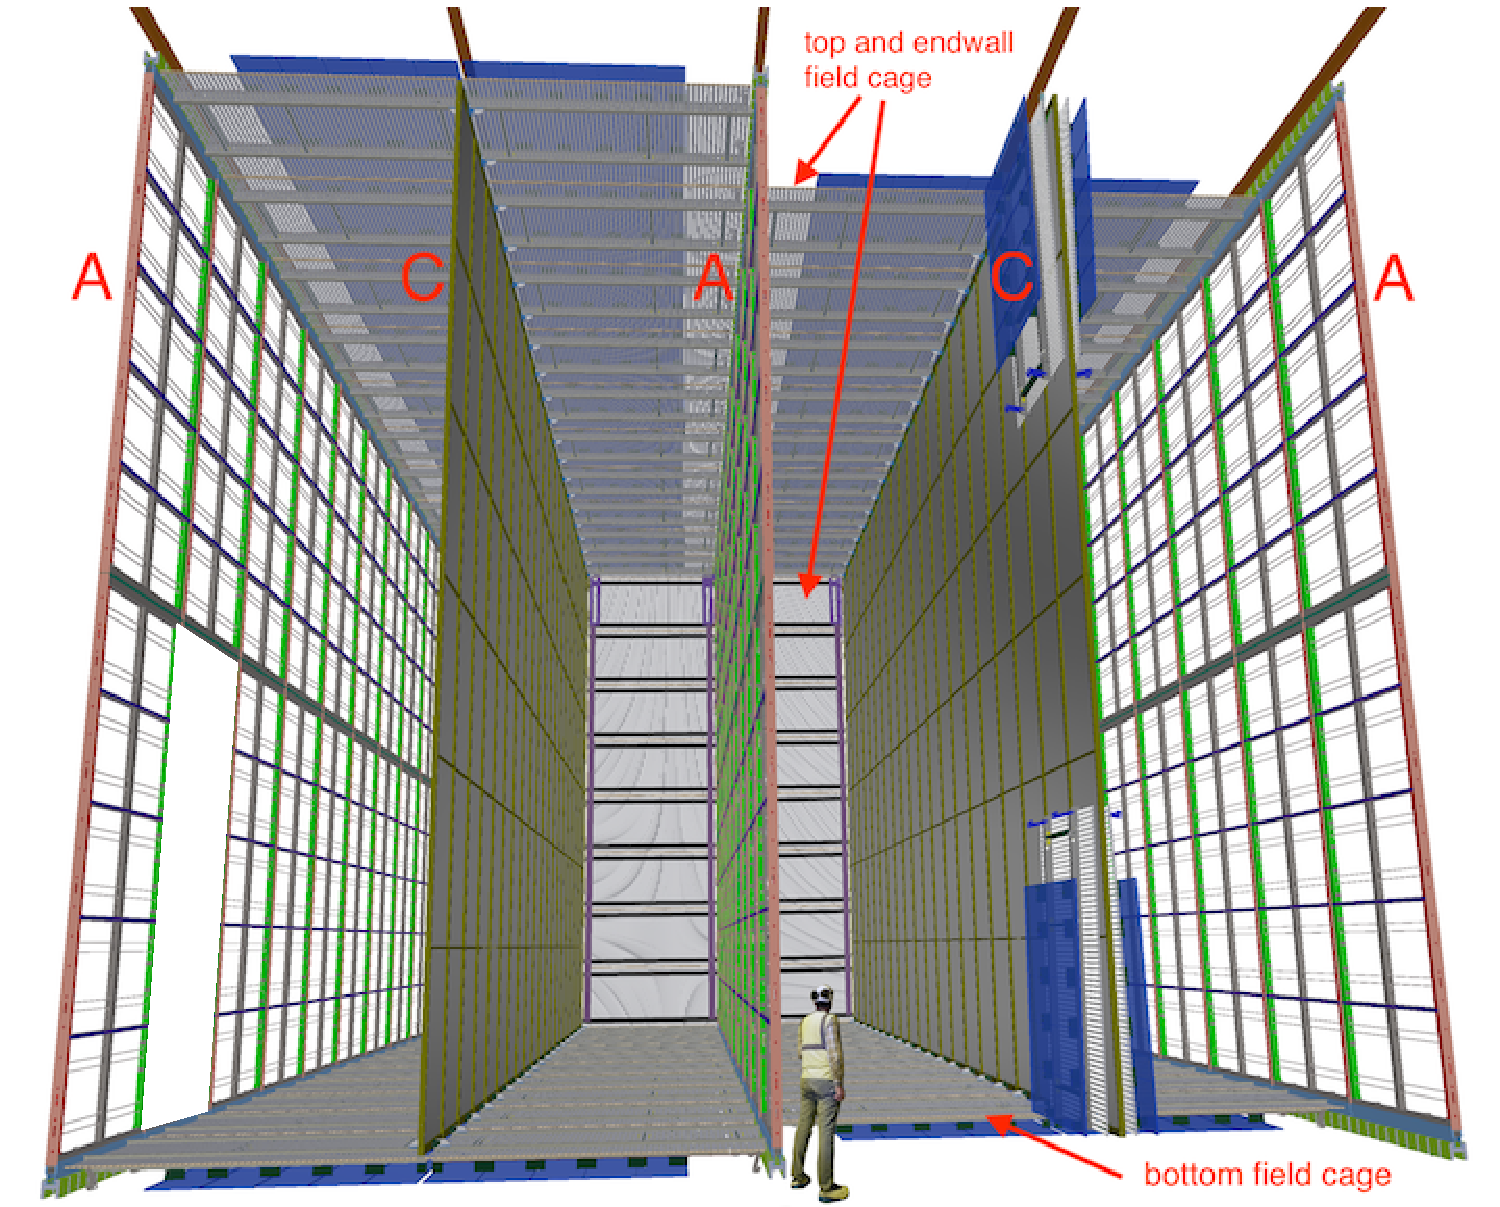
\includegraphics[height=0.35\textwidth]{graphics/IntroFigures/Fig_03b_DUNESchematic.pdf}
\caption{Left) A far detector cryostat that houses a 10 kT \dword{fd} module. The figure of a person indicates the scale.  Right) A 10kt  \dword{dune} \dword{fd} \dword{spmod}, showing the alternating 58 m long (into the page), 12 m high anode (A) and cathode (C) planes, as well as the field cage that surrounds the drift regions between the anode and cathode planes. The blank area on the left side was added to show the profile of a single \dword{apa}.}
\label{DUNESchematic}
\end{figure}

\section{ProtoDUNE tests at CERN}

Building an experiment of this size requires an extensive period of prototyping.   The Argoneut\cite{Acciarri:2018myr}, MicroBooNE\cite{microboone} and ICARUS\cite{icarus} collaborations have demonstrated the capabilities of large liquid Argon \dword{tpc}s for neutrino detection on scales between 1 and 500 ton fiducial mass.  In preparation for the \dword{dune} experiment, a campaign testing proposed DUNE components in 700 ton detectors in the EHN1 hadronic test-beam was launched at CERN in 2018.  Both single-phase and dual-phase prototypes were constructed and tested. % We have tested the full data taking chain from detector construction to full offline reconstruction and analysis of data. 

\subsection{ProtoDUNE Single Phase}
The \dword{pdsp} experiment began taking data at CERN in late 2018.  \dword{pdsp} uses single-phase technology where ionization electrons are collected directly from the liquid argon. The readout system consists of  Anode Plane Assemblies (\dword{apa})s which each have 3 layers of wires arranged in different directions. Each layer contains 800-1200  wires spaced 0.5 cm apart. Electrons drift from the original interaction in the Argon, through a strong electric field, to the wire planes and induce signals.  The location in the plane of hit wires gives one coordinate, the time the signal takes to drift to the wire from the original interaction measures a second coordinate.  The third coordinate is derived by combining information from overlaps of signals in the 3 different wire layers.  Signals are amplified electronically and then digitized.  Figure \ref{tpcconcept} illustrates the operation of a generic \dword{lartpc}.

Horizontal drift single-phase technology with \dword{apa} readout, similar to those used in \dword{pdsp}  will be used for the first of the four \dword{fd} modules. 

\begin{figure}[ht]
    \centering
%    \subfloat[EM]{\label{Blob1_const}
\includegraphics[trim={0cm 0.6cm 2.5cm 0.7cm},clip,height=8cm]{graphics/IntroFigures/Fig_04_LArTPC_Concept.png}%\includegraphics[trim={1.3cm 0.6cm 2.5cm 0.7cm},clip,height=3.5cm]{h_ptmumichel_1track_const_.pdf}
    \caption{Diagram  from  \protect{\cite{ Acciarri:2017sde}}  illustrating the signal formation in a LArTPC with three wire planes~\cite{Acciarri:2016smi}. For simplicity, the signal in the first U induction plane is omitted in the illustration. }%Planes are positioned in the order U, V, Y with the Y plane being farthest from the cathode plane}
    \label{tpcconcept}
    \end{figure}

The \dword{pdsp} detector consists of a 700 ton volume of liquid argon with a cathode plane in the center and 3 \dword{apa}s mounted on  each  edge of the liquid volume. The electric field is horizontal so this technology is designated \dword{hd}.   The drift distance is  3 m with  a nominal voltage of 180kV  across that distance.  Each \dword{apa} has 2560 channels and each channel reads out a 12-bit \dword{adc} every 0.5 $\mu$sec.   For \dword{pdsp} the readout time appropriate for a 3 m drift was set to 3 msec, resulting in 6000 12-bit samples per channel.  The total data size for six \dword{apa}s is thus 140 MB with additional header and data from photon and external tagging systems bringing the nominal event size up to around 180 MB.  Lossless compression of the \dword{tpc} readout was implemented in the data acquisition system, resulting in a final compressed event size of around 75 MB. 

The test-beam ran at rates of up to 25 Hz over a period of 6 weeks at beam momenta between 0.5 and 7 GeV/c.  Time of flight and Cherenkov counters in the beamline provided beam flavor tagging.  Around 8M total `physics' events were written, with around 3M having beam tag information.  In total  850 TB of raw test-beam data were written, along with one PB of commissioning and cosmic data. These data were successfully cataloged and written to storage at both CERN and Fermilab at rates of up to 2 GB/sec.   

Thanks to significant prior effort in the \dword{lar} computing and algorithms community, reconstruction software was ready to go and the first reconstruction pass began soon after data taking started and was complete within two weeks of the end of data taking.  Those results were extremely useful in demonstrating the capabilities of the detector and summarized in Volume II of the \dword{tdr}\cite{Abi:2020evt}.  A second pass, with improved treatment of instrumental effects ranging from stuck bits to 2-D deconvolution to correction for space charge effects was completed in late 2019. Another pass with major improvements to the electrostatic modeling and reconstruction algorithms was launced in 2021. 

%\dword{pdsp} Reconstruction - from raw data to beam interactions and cosmics full reconstructed with 80-90\% efficiency - has been performed twice over the 8M interactions recorded during the test-beam runs. 
Figure \ref{deconvolution} illustrates the signal processing stage of reconstruction, where raw ADC signals have noise and stuck bits removed and are then deconvoluted to yield gaussian hit candidates. Figures \ref{wire-cell-bee} and \ref{pandora} illustrate full pattern recognition and event reconstruction. 

While \dword{lartpc}s benefit from fine granularity and a uniform detector medium, diffusion, argon purity, fluid flow and the build up of space charge in the active medium can all introduce distortions into the detector response.  These effects have all been simulated and tested in the \dword{pdsp} data. 

Compressed raw input event records were of order 75 MB in size and took 500-600 seconds to reconstruct, of which around 180 sec was signal processing and the remainder high level reconstruction dominated by 40-60 cosmic rays per readout.  Memory footprints for data processing ranged between 2.5 and 4 GB.  Output event  record sizes were reduced to 22 MB by dropping the raw waveforms after hit finding.   Data reconstruction campaigns took of order 4-6 weeks (similar to the original data taking) and utilized up to 15,000 cores on \dword{osg} and \dword{wlcg} resources.  Job submission was done through the POMS\cite{poms} job management system developed at Fermilab. POMS supports submissions to FNAL dedicated resources and selected OSG and WLCG sites.  Figure \ref{sites} shows the distribution of wall hours used for reconstruction in 2019. 

For reconstruction, data were streamed via {\tt xrootd}\cite{Behrmann:2011zz} from \dword{dcache} storage at Fermilab to the remote sites. Despite individual processing jobs taking 15-30 hrs to complete, network interruptions rarely caused job failures. 


 

\begin{figure}[ht]
\centering
%[Raw  and deconvolved induction U-plane signals from a ProtoDUNE-SP event]
%{pDUNE_sp_example}
\includegraphics[width=0.49\textwidth]{graphics/IntroFigures/Fig_05a_protodune_raw_u.pdf}
\includegraphics[width=0.49\textwidth]{graphics/IntroFigures/Fig_05b_protodune_decon_u.pdf}
\caption{Comparison of raw (left) and deconvolved induction U-plane signals (right) before and after 
the signal processing procedure from a \dword{pdsp} event. The bipolar shape with red (blue) color representing
positive (negative) signals is converted to the unipolar shape after the \twod deconvolution.}
\label{deconvolution}
\end{figure}

\begin{figure}
%[\threed display of interaction in ProtoDUNE-SP]
\centering
\includegraphics[width=0.9\textwidth]{graphics/IntroFigures/Fig_06_bee_event.png}
\caption {The \dword{pdsp} detector (gray box) showing 
the direction of the particle beam (yellow line on the very far left) and the outlines of the six \dword{apa}s. Cosmic rays
can be seen throughout the white box, while the red box highlights the beam region of interest with an interaction of the 7 GeV beam. 
The \threed points are obtained using the Space~Point~Solver reconstruction algorithm. }
\label{wire-cell-bee}
\end{figure}

\begin{figure}
\centering
\includegraphics[width=0.8\textwidth]{graphics/IntroFigures/Fig_07_pandora.png}
\caption{Pandora \protect{\cite{Acciarri:2017hat}} reconstruction of cosmic rays and beam interaction in a \dword{pdsp} event. The left side of the figure shows the full detector volume with all interactions, including cosmic rays and the right side shows the identified beam interaction.}
\label{pandora}
\end{figure}


\begin{figure}[ht]
\begin{center}
%\includegraphics[height=0.5\textwidth]{Fig_08a_Picture1.png}
%\includegraphics[height=0.5\textwidth]{Fig_08b_Picture2.png}
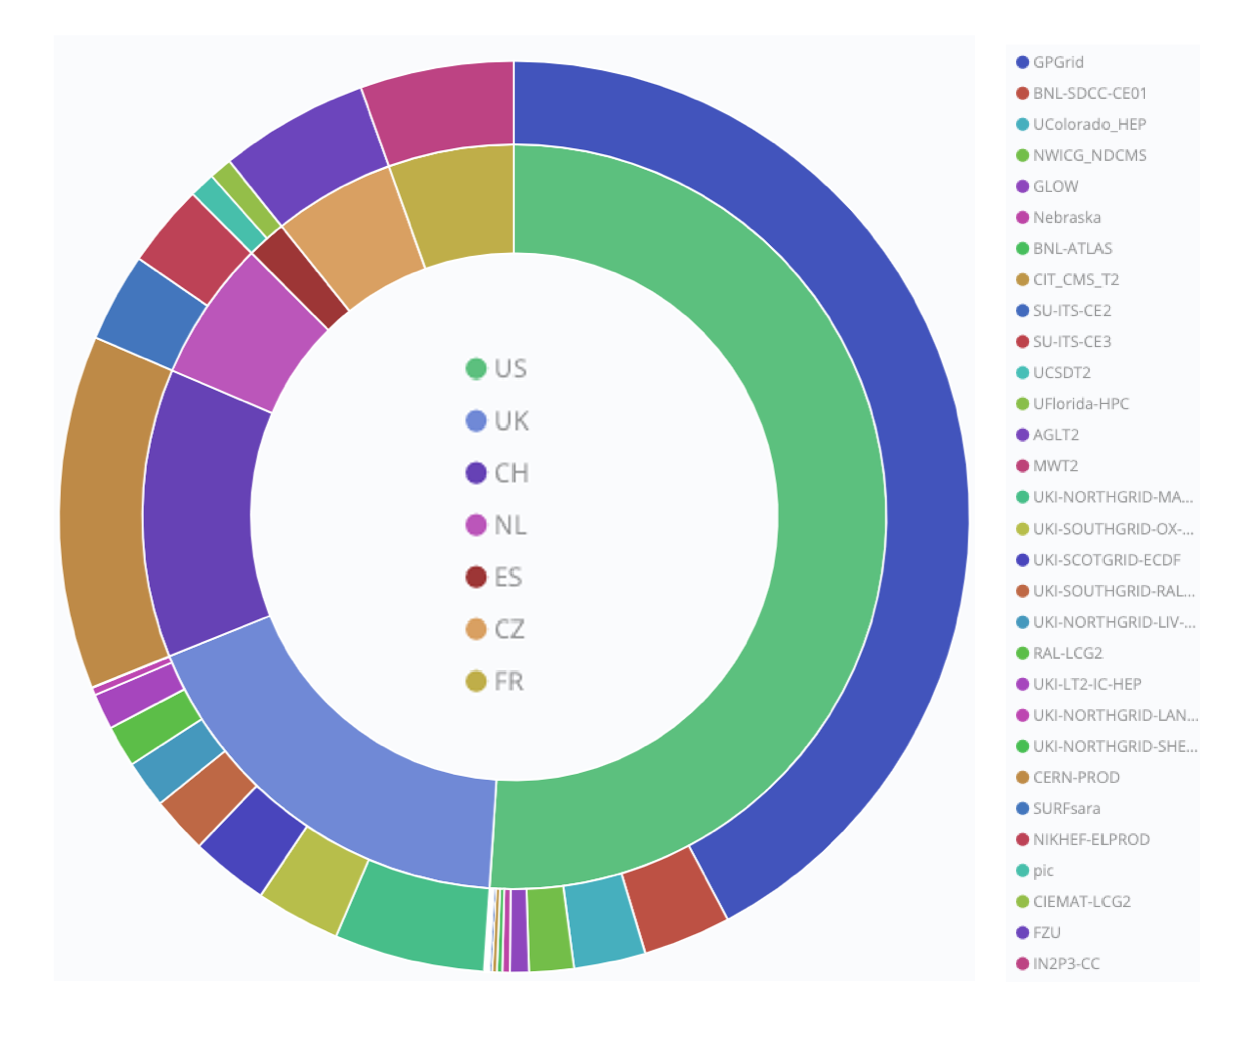
\includegraphics[height=0.65\textwidth]{graphics/IntroFigures/Fig_8.pdf}
\caption{Reconstruction and simulation processing distribution across sites for DUNE production in calendar 2019.  The inner circle shows national contributions while the outer circle shows individual site contributions.}
\label{sites}
\end{center}
\end{figure}

\subsection{ProtoDUNE Dual-Phase}

%The \dword{pddp} detector began taking data using cosmic rays in August 2019.  Thanks to preceding data challenges, those data have been successfully integrated into the full data cataloging and reconstruction chains and are now being reconstructed as they arrive.   The \dword{pddp} technology locates the readout systems above a thin layer of argon gas above the liquid argon surface.  This gas layer allows an external electric field to accelerate the electrons and produce gas amplification.  The result is a substantial increase in signal-to-noise in the resulting signals, at the cost of longer electron drifts from the bottom of the liquid volume.  Figure \ref{dpevent} illustrates early data from \dword{pddp}. 

The basic operating principle of \dword{pddp} is shown in figure \ref{dp_principle}. Charged particles that traverse the active volume of the LArTPC ionize the medium while also producing scintillation
light. The ionization electrons drift in the vertical direction toward an extraction grid just below the liquid-vapor interface. 
After reaching the grid,
an E field stronger than the drift field extracts the electrons from the liquid up into the gas phase.
Once in the gas, electrons encounter micro-pattern gas detectors, called \dwords{lem}, with high-field regions. The \dwords{lem} amplify the electrons in avalanches that occur in these
high-field regions. The amplified charge is then collected and recorded on a 2D anode consisting
of two sets of 3.125 mm-pitch gold-plated copper strips that provide the x and y coordinates (and
thus two views) of an event.   
\begin{figure}
\centering
\includegraphics[width=0.85\textwidth]{graphics/IntroFigures/Fig_11_protodune-dp-principle.png}
\caption {Principle of DP readout (left), and thicknesses and HV values for electron extraction from liquid to gaseous argon, their
multiplication by LEMs, and their collection on the x and y readout anode plane (right) The HV values are
indicated for a drift field of 0.5 kV/cm in LAr.}
\label{dp_principle}
\end{figure}
The readout area surface is 6x6 m$^2$, subdivided into four $3\times3$ m$^2$  \dwords{crp}. Each \dword{crp} is an independent detector element insuring electron extraction, amplification, and collection. 
The readout channels (7680)  are read by at 12 bits ADC every 0.4 $\mu$sec. 
The \dword{pddp} detector   consists of a 700 ton volume of liquid argon, with  a drift length of 6m, corresponding to a full drift window of 4ms (10000 samples).

The \dword{pddp} detector began taking data using cosmic rays in August 2019. Thanks to preceding data challenges, those data have been successfully integrated into the full data cataloging and reconstruction chains and are now being reconstructed as they become available.
A total of 1.9M events has been collected; the size of the raw data files (run sequence files) corresponds 3GB, each file containing 30 events. Cosmic ray events are displayed in Figure \ref{dpevent}: on
the left an horizontal muon track is shown with the corresponding waveform on a channel, giving an
idea of the low noise conditions. An event including an electromagnetic shower and two muon decays
and an event with an example of multiple hadronic interactions in a shower are shown on the right.
 
\begin{figure}
\centering
\includegraphics[width=0.85\textwidth]{graphics/IntroFigures/Fig_09_protodune-dp-event.png}
\caption {Cosmic ray data from the dual phase prototype}
\label{dpevent}
\end{figure}
All data ($\sim$ 200TB) taken during different campaigns   have been copied to \dword{fnal}. A subsample is composed by data sets taken during detector transient conditions, motivated by various specific testing needs;  all cosmic ray data taken in well defined and stable detector conditions in 2019 and 2020 ($\approx$  377K events) have been processed with \dword{larsoft} by performing the reconstruction of hits and 2D tracks. A second pass, including Pandora reconstruction algorithms, started in Spring 2021. 
The memory footprint is between 1.9 and 2.5 GB
As for \dword{pdsp}, job submission was done through \dword{poms}.

In the fall 2020 the dual-phase design evolved to the \dword{vd} concept. The \dword{vd} incorporates many of the design aspects developed for the dual-phase, such as the \dwords{crp};   the  main  difference  with  respect  to  the  dual-phase  design  is   the  removal  of  the  extraction  stage  to  the  gas  phase  and  the  subsequent  charge  amplification  stage.   This  change eliminates the grid immersed in the liquid and biased at high voltage in order to define the field needed to transfer the electrons from the liquid to the gas phase and the \dwords{lem} used to amplify the signal. The vertical drift \dword{crp} keeps the concept of charge readout performed with strips implemented on segmented PCB anodes while replacing
 the \dword{lem} micro-pattern detectors, which operated in the argon gas phase and coupled to the anode printed circuit boards with charge collection strips, with perforated anodes immersed in the \dword{lar}
\begin{figure}
\centering
\includegraphics[width=0.85\textwidth]{graphics/IntroFigures/Fig_13_VD_solution.png}
\caption {Vertical drift solution with PCB-based charge readout}
\label{vd_principle}
\end{figure}
 Figure \ref{vd_principle} illustrates the \dword{pcb}-based charge readout concept. The electron drift direction is vertical.
Two separate drift volumes of 6.5m are defined by a cathode plane at roughly mid-height in the
detector volume. Ionization electrons above the cathode will drift upwards; ionization electrons in the liquid below the cathode will drift downwards.
The Vertical Drift  prototype components will undergo testing in 2021 and 2022.  A full prototype, known as ``Module 0", is expected to be completed and  installed 
 inside the NP02 cryostat in 2022 and 2023. Long-term operation and full characterization with a charged particle beam will follow. 



\subsection{Conclusions from prototype tests}
\dword{protodune} prototype runs are ongoing and will continue through beam tests in 2022 at \dword{cern}.  Data cataloging, movement and storage techniques were tested before the start of the \dword{pdsp} and \dword{pddp}  runs and were able to handle the full rate of the experiments.   Reconstruction algorithms were also in place on time and were able to produce early results that led to increased understanding of the detector and improved calibrations for a second iteration.  These tests also identified some deficiencies in our infrastructure, including incomplete schemes for the transmission of configuration and conditions information between hardware operations and  offline computing.  The test-beam runs have been extremely valuable in allowing us to determine which variables are important to transmit and in designing improved systems for gathering and storing that information. 

An additional beam run of  \dword{pdsp} is planned for 2022, with a cosmic test of the vertical drift design to follow in 2023, allowing further development and testing of our computing infrastructure before the full detector comes online in the late 2020's. 


\section{On to full DUNE}\label{sec:intro-fd}

The full DUNE \dword{fd} will begin with one single phase \dword {hd} module to be installed at Homestake starting in the middle of  this decade.  A second \dword{vd} module will be installed and commissioned in parallel.  High intensity neutrino and anti-neutrino beams should arrive after a year or so of commissioning of the detector and \dword{lbnf} beamline.  The first \dword{hd} module will largely resemble a scaled up version of \dword{pdsp} with 150 \dword{apa}s distributed 2-deep at the center and long edges of the cryostat.   The argon volume will be $15\times14\times62$ m$^3$ with a fiducial mass of 10kT.  Section \ref{sec:est:FD} summarizes the expected event rates and data volumes for the first two modules.  Two additional detector modules, possibly with novel technologies, beyond the first two will be added later. For now, we assume that data volumes and rates coming from other technologies will be less than or equal to the single-phase values. 



The detectors should be sensitive to neutrino interactions and radioactive decays above an energy threshold of order 5 MeV.  Unambiguous triggering may require a somewhat higher threshold  to avoid false triggers due to $^{39}$Ar decays,  but beam interactions in the 500-10,000 MeV range should have almost perfect detection efficiency. Sophisticated triggering algorithms should also allow standalone detection of astrophysical sources, including higher energy solar neutrinos and supernova candidates. 

The data rates will be dominated by 4,500 cosmic rays expected per module/day.  These events are vital for monitoring and aligning the detector.  The next most significant source of events will be calibration campaigns with radioactive and neutron sources and lasers.  In all cases, the goal is to gather data from the full volume of the detector with as fine a granularity as possible. 

Beam interactions themselves are expected to be quite rare, occurring in only 1/2000 beam gates ($\simeq$ 2/hr)  Extraction of oscillation parameters will require both the powerful electron background rejection, discussed in the previous section,  and precise calibration of the energy scale of the experiment, hence the much larger calibration samples.

Beam and cosmic ray interactions are reasonably localized in time and space, involving a small fraction of a module over a few milliseconds.  This can, in principle, allow significant reduction in data size without loss of physics information if suitable triggers are used.

\subsubsection{Low energy phenomena - solar/neutron decay} \fixme{ Need someone to write about solar/BSM signature}

\subsubsection{Supernova candidates}\label{sec:supernova}


 \begin{figure}
 \begin{center}
 \includegraphics[height=0.3\textwidth]{graphics/IntroFigures/Fig_10a_Picture3.png} \hskip 1 in
\includegraphics[height=0.5\textwidth]{graphics/IntroFigures/Fig_10b_Picture4.png}
 \caption{Left) a charged current interaction of a 30 MeV energy electron neutrino in the DUNE Far Detector.  Right) a neutral current excitation and de-excitation of an Ar nucleus by a  10 MeV neutrino.}
 \label{blips}
 \end{center}
 \end{figure}


Supernova candidates pose a unique problem for data acquisition and reconstruction.  Supernova physics in DUNE is discussed in some detail in the \dword{tdr}\cite{ Abi:2020evt} and only summarized here. A classic core-collapse supernova 10 kpc away would be expected to yield around 3,000  charged-current electron neutrino interactions across 4 detector modules. Supernova candidates will be quite different from beam interactions, with small interactions with energies in the 5-30 MeV range spread across the full volume of the detectors over many seconds, in contrast to the localized, coincident,  500-10,000 MeV signature of beam neutrino interactions. These differences impose interesting requirements on the data acquisition and computing models for the experiment.  


Supernova physics and its influence on neutrino emission are not fully understood and will result in significant modulations of the event rates for different neutrino types  over the few tens of seconds of the burst.  DUNE's fine-grained tracking should allow significant pointing power with the most optimistic scenario of four modules and high electron neutrino fraction yielding pointing resolutions of less than 5 degrees.   Figure \ref{blips} illustrates simulated signatures of supernova neutrino interactions in the far detector. The ability to produce a reasonably fast pointing signal would be extremely valuable to optical astronomers doing followup, especially if a supernova was in a region where dust masks the primary optical signal.   The need to be alert to supernovae and to quickly transfer and process the data imposes significant requirements on triggering, data transfer and reconstruction beyond those imposed by the more regular beam-based oscillation physics.   For example, a compressed supernova readout of all four modules will be of order 184 TB in size and take a minimum of 4 hrs to transfer over a 100 Gbs network,  and then take of order 130,000 CPU-hrs for signal processing at present speeds.  If processing takes the same time as transfer, a peak of 30,000 cores would be needed. 

\section{Near Detectors}

High precision oscillation physics requires a near detector system to allow measurement of the original neutrino flux and improved understanding of neutrino interaction physics.  The DUNE  collaboration is proposing a suite of near detectors optimized for these two goals. 
 
 The near detectors will be located in an enclosure on the Fermilab site 574 meters from the target and will be exposed to the DUNE neutrino beam.    Interaction rates per spill (at 0.83 Hz) are expected to be very large, with 40-60 interactions per spill, including muons originating from interactions in material upstream of the fiducial volumes. Figure \ref{beamline} shows the beamline and location of the near detectors on the Fermilab site. There are three major subsystems:
 A pixel readout liquid argon detector, \dword{ndlar}, is  the most upstream of the three sub-detectors shown in Figure \ref{nd}, where the beam propagates  from right to left. Immediately downstream of \dword{ndlar} is the gaseous liquid argon detector, \dword{ndgar}, which serves \dword{ndlar} as  a muon spectrometer and allows more detailed study of neutrino interactions that occur within its gas volume. Beyond \dword{ndgar}, is the \dword{sand} component of the ND that acts as a beam monitor. %Figure \ref{nd} shows the three \dword{nd} subdetectors in the near enclosure. 
 
 \begin{figure}[ht]
     \centering
     \includegraphics[height=0.3\textwidth]{graphics/IntroFigures/beamline-sideview.png}
     \caption{The LBNF neutrino beamline on the Fermilab site. The near detectors will be situated 574 m from the target and 62 m below grade.}
     \label{beamline}
 \end{figure}
 
 \begin{figure}[ht]
     \centering
     \includegraphics[height=0.5\textwidth]{graphics/IntroFigures/All3Detectors.pdf}
     \caption{The near detector systems in an on-axis configuration.  The beam enters from the lower right in this view. The \dword{sand} scintillating beam monitor remains at beam center while the pixel ND-LAr TPC detector and gaseous ND-GAr TPC detectors can be moved off-axis to make detailed studies of the neutrino flux at multiple angles.  }
     \label{nd}
 \end{figure}
 
 \subsection{pixel LArTPC - ND-Lar}
 
 As the target material in the Deep Underground Neutrino Experiment (DUNE) far detectors is liquid argon, optimal cancellation of systematic uncertainties between the near and far detectors requires that the near detector include a liquid argon component to match the \dword{fd}.  However, at the intense neutrino flux and high event rate in the ND region, occupancies will be too high to allow the 2-D readout provided by conventional wire planes. A new ArgonCube  technology has been developed that allows pixelized charge readout  and provides unambiguous 3D imaging of  particle interactions.  The ND-LAr component of the DUNE ND is made up of a configuration of ArgonCube LArTPCs  large enough to provide the required hadronic shower containment and statistics.  %The 5 m (along beam)×7 m (horizontal,  transverse to beam)×3 m (height), 67 t fiducial mass, of ND-LAr are optimized primarily for  hadronic containment under the assumption that ND-GAr will measure the sign and momentum  of downstream exiting muons. Figure 2.2 shows the arrangement of modules in the crystat for  ND-LAr.  Section 2.2 gives a discussion of the physics consideration
 
 The pixel liquid argon detector will have 12~million $3\times 3$~mm$^2$ pixel channels and $\sim$4200~photon detector channels.  The LArTPC will read out only pulse times and integrals, in contrast to the far detector which reads out every time slice.  The photon detectors will, however, read out complete wave-forms.   A total of 3~MB of uncompressed data is anticipated per spill from the TPC with 5-MB from the photon detectors leading to an estimate of 144 TB/year for uncompressed in-spill data. Calibrations and cosmic ray data increase that data volume by around 20\%.

% For calibrations, 300 runs are assumed to be taken per year, each generating 10~GB of data, for the TPC, and a similar set of runs for the photon detectors.  These runs include pulser runs, laser runs, radioactive source runs, or other special-condition runs that require taking data outside of the regular spills.  Since they are not tied to the spill timing structure, they can be collected at higher trigger rates and take less time.

% In addition to the beam data, cosmic rays will contribute to the data volume.  For the \dword{ndlar} geometry in the ND hall, the anticipated rate
% of cosmic rays is 100~Hz.  If all cosmic ray data were collected, the data volume would be approximately 1~MB/sec.  The scenario considered here is to
% collect one spill's worth of cosmic ray data for every ten beam spills, for a data volume of 6.3 TB per year.  While the activity on the cosmic-ray triggers is expected to be much less than that on a beam spill, it is assumed that the cosmic-ray triggering will continue even when the beam is off.

% The TPC-only out-of-spill and calibration numbers have been scaled by 8/3 to account for photon detector data, assuming full waveform readout in these samples, yielding the same ratio as in-spill data and the same compression. 

\subsection{Near Detector Gaseous Argon TPC}
\label{sec:comp-dataestimates-mpd}

The \dword{ndgar} is a magnetized detector system consisting of a high-pressure gaseous argon TPC  (HPgTPC) surrounded by an electromagnetic calorimeter (ECAL) and a muon system. The \dword{ndgar} measures the momentum and sign of charged particles exiting the ND-LAr. In addition, for neutrino interactions occurring in the \dword{ndgar} itself, higher resolution and lower momentum thresholds can be achieved for charged particle tracks, leading to improved neutrino interaction models. This capability enables further constraints of systematic uncertainties for long-baseline neutrino  oscillation analyses.

The \dword{ndgar} is composed of 678,136 readout pads in the TPC, and approximately 3~million channels in the \dword{ecal}.  Approximately one in five spills will generate an interaction in the gas TPC, but particles entering the gas from interactions in the \dword{ecal} will provide the bulk of the data volume.  The readout strategy will be similar to the LArTPC, with only time and integral recorded. A  data volume of 2 MB of uncompressed data per spill is expected from the TPC.  The calorimeter is expected to contribute approximately 1~MB per spill of uncompressed data.

% For calibrations, 300 runs per year generating 10~GB of data per run are assumed for the TPC, and a similarly-sized set of calibration runs are assumed for the \dword{ecal}.  Cosmic rays are expected to be collected between spills and when the beam is off.



\subsubsection{SAND}
\label{sec:comp-dataestimates-sand}
%The 3rd detector subsystem is the \dword{sand}, a scintillator based monitor, consists of a 3-D pixelated scintillator detector, an electromagnetic calorimeter and XXX

The \dword{sand} component of the near detector (ND)'s primary function is the primary beam flux monitor.   SAND consists of an active scintillator target \dword{3dst} followed by a tracking system immersed in a solenoidal superconducting magnet  and  a $4\pi$ electromagnetic calorimeter.

\dword{sand}'s \dword{3dst} calorimeter component is composed of 11,520,000 $1\times 1\times 1$~cm$^3$ scintillating cubes, read out by 153,600 fibers.  There are expected to be approximately 2,160 hits per spill with a total of 0.13 MB of data per spill.  The  \dword{ecal}~\cite{Adinolfi:2002zx} uses 4,850 PMTs, with an estimated 5,500 total hits per spill or 33 kB of packed data per spill.   The data volume from SAND is 4.3 TB/year with these assumptions.  The amount of data from out-of-spill cosmic rays is estimated to be 20\% of that of the in-spill data, or approximately 1 TB.  The data volume from SAND is significantly smaller than that from the \dword{ndlar} and the \dword{ndgar} due to the relative sizes of the three-dimensional tracking volumes and the segmentation choices.




% Test using \dword{tms}

%\subsection{Simulation challenges}

\section{Relation of Physics Goals and Computing Challenges}

The \dword{DUNE}physics program drives several detector characteristics that pose novel computing challenges.  While the overall data volumes are smaller than those routinely handled by the large LHC experiments, the remote detector site and unique physics goals present novel computing challenges. 

\begin{description}
\item{\bf Fine segmentation needed for electron-photon discrimination: \\}   The primary goal of the DUNE/LBNF long baseline experiment is measurement of $\nu_\mu\rightarrow\nu_e$ and $\nubar_\mu\rightarrow\nubar_e$
oscillation probabilities for GeV scale accelerator neutrinos.   These oscillation probabilities are intrinsically low and sensitive to backgrounds where the neutral current process  $\nu_mu+A\rightarrow\nu_mu+\gamma+X$
produces a photon which fakes an oscillation signal.  Fine detector segmentation is necessary to distinguish between these scenarios. Figure \ref{fig:Argoneut} illustrates this capability. The need for sub-cm-level segmentation drives the technology choice of LArTPC's and hence the number of channels.   
\item{\bf Low Energy Thresholds for Astrophysical Aeutrinos: \\}
Other important physics goals are the detection of astrophysical neutrinos from the sun, possible supernovae, atmospheric cosmic rays and physics beyond the standard model (BSM) signatures in the \dword{fd}.  Astrophysical neutrinos produce lower energy signatures, in the 1-30 MeV range. Extracting such signals, near the noise threshold of the detector and in the presence of radiological backgrounds, requires careful attention to signal processing and zero-suppression for the \dword{fd} \dword{tpc} and \dword{pd} wave forms.  The need to optimize the low energy threshold drives our need to carefully record waveforms with minimal processing. 

\item{\bf Precise Energy Calibrations:\\}
An additional challenge in oscillation physics is the need for accurate energy calibration in order to utilize the energy spectrum of the reconstructed neutrinos to further constrain oscillation parameters. While \dword{lar} detectors have a reputation for stability, the large volumes, complex electric field configurations, liquid motion and potential variations in electron lifetime and drift velocity make large calibration data samples which span the full \dword{fd} detector volume necessary.  Large cosmic ray and artificial calibration samples will dominate the total data volumes from the \dword{fd}. 

\item{\bf Supernovae:\\}A supernova candidate will generate 115  TB of data per module. This means tens of thousands of data files produced over a 100 s period. These data must be recorded at low energy threshold due to the expected energy range but must also be analyzed quickly and coherently in order to measure the time evolution of neutrino emissions, which carries invaluable information about the supernova process itself. In addition, if \dword{dune} can quickly analyze charged-current interactions, we can provide pointing information to telescopes for followup.  Supernova physics drives the need for fast data transmission from the \dword{fd} to compute facilities and for robust tracking of data movement so that a full picture of the supernova interaction can be reassembled after signal processing. 

\item{\bf Near Detector Integration: \\}
While the \dword{fd} detectors produce large data volumes, the detectors themselves are reasonably simple, consisting of a small number of technologies and large numbers of repeating components.  The \dword{nd} is much more complex. 

The \dword{nd} use case is similar to other fixed target experiments such as \dword{sbnd} at \dword{fnal} and \dword{compass} at \dword{cern}.  The main computing challenge for the \dword{nd} will be integration of a large number of disparate detector technologies into a coherent whole. Here careful attention to simulation, detector geometry and configuration and code management will be the major challenges. 

\item{\bf Analysis and Parameter Extraction:\\}
\dword{dune} has over one thousand collaborators spread across four continents. Those collaborators will want to analyze our data over several decades. Fortunately, once reconstruction has been done, neutrino interaction samples are generally simpler than event records at colliders and should be analyzable locally.  However, final parameter extraction  using large numbers of nuisance parameters remains a computationally intense problem and will require significant resources. 



\end{description}

\end{document}

\cleardoublepage




\documentclass[../main-00.tex]{subfiles}
\begin{document}

\chapter{Data and Processing Volume Estimates \hideme{Schellman, Junk, Muether}}
\label{ch:est}
\fixme{Heidi: moved tables of numbers from intro to here.  Still needs better organization}
In this chapter we will describe the assumptions that go into a bottoms-up estimate of data volumes and describe possible methods of reducing the total volumes while retaining physics capabilities. 

\section{Introduction}

% \begin{dunetable}
% [Data Sizes and Rates]
%  {l |r r r }
%  {tab:volumes}
%  {Data sizes and rates for different processes in each far detector module.  Uncompressed data sizes are given. As readouts will be self-triggering an extended 5.4 ms readout window is used instead of the 3ms for the triggered \dword{pdsp} runs.  We assume beam uptime of 50\% and 100\% uptime for non-beam science. These numbers are derived from references \protect{\cite{bib:docdb16028}}and \protect{\cite{bib:docdb14983}}.}
% % 5
%  Process & Rate/module & \qquad size/instance &\qquad  size/module/year\\ \toprowrule
%  %
%  Beam event & 41/day & 6 GB&47 TB/year\\
%  Cosmic rays &4,500/day&  6 GB& 9.7 PB/year\\
%  Supernova trigger& 1/month& 115 TB& 1.4 PB/year\\
%  Calibrations&2/year&750 TB& 1.5 PB/year\\
%  %\toprowrule 
%  Total& & &12.9 PB/year\\
%  \end{dunetable}




%  \subsection{Supernova candidates}


%  \begin{figure}
%  \begin{center}
%  \includegraphics[height=0.3\textwidth]{graphics/IntroFigures/Fig_10a_Picture3.png} \hskip 1 in
% \includegraphics[height=0.5\textwidth]{graphics/IntroFigures/Fig_10b_Picture4.png}
%  \caption{Left) a charged current interaction of a 30 MeV energy electron neutrino in the DUNE Far Detector.  Right) a neutral current excitation and de-excitation of an Ar nucleus by a  10 MeV neutrino.}
%  \label{blips}
%  \end{center}
%  \end{figure}


% Supernova candidates pose a unique problem for data acquisition and reconstruction.  Supernova physics in DUNE is discussed in some detail in the \dword{tdr}\cite{ Abi:2020evt} and only summarized here. A classic core-collapse supernova 10 kpc away would be expected to yield around 3,000  charged-current electron neutrino interactions across 4 detector modules.  The oscillation physics is not fully understand and can result in significant modulations of the event rates for different neutrino types  over the few tens of seconds of the burst.  DUNE's fine-grained tracking should allow significant pointing power with the most optimistic scenario of four modules and high electron neutrino fraction yielding pointing resolutions of less than 5 degrees.   Figure \ref{blips} illustrates simulated signatures of supernova neutrino interactions in the far detector. The ability to produce a reasonably fast pointing signal would be extremely valuable to optical astronomers doing followup, especially if a supernova was in a region where dust masks the primary optical signal.   The need to be alert to supernovae and to quickly transfer and process the data imposes significant requirements on triggering, data transfer and reconstruction beyond those imposed by the more regular beam-based oscillation physics.   For example, a compressed supernova readout of all four modules will be of order 184 TB in size and take a minimum of 4 hrs to transfer over a 100 Gbs network,  and then take of order 130,000 CPU-hrs for signal processing at present speeds.  If processing takes the same time as transfer, a peak of 30,000 cores would be needed. 


% \fixme{Move or copy to the data volumes section}
% \begin{dunetable}
% [Useful FD Data Quantities]
% {|l  l |c       | l |}
% {tab:exec-comp-bigpicture-es}
% {Useful quantities for computing estimates for \dword{sp}
% readout. For  sparse \dword{fd} events, the pattern recognition phase, which scales with occupancy is expected to be substantially faster than the signal processing phase which scales with detector size.  }%
% Quantity&&\qquad Value \qquad&Explanation\qquad \qquad\\
% \toprowrule
% {\bf Far Detector Beam:}&&&\\ 
% &Single APA readout &41.5 MB& Uncompressed 5.4 ms\\ 
% &Single APA readout &16.6 MB& $\times 2.5$ compression\\
% &APAs per module& 150&\\
% &Full module readout &6.22  GB& Uncompressed 5.4 ms\\ 
% &Beam rep. rate&0.83 Hz&Untriggered\\  
% Signal processing &CPU time/APA&40 sec&from MC/ProtoDUNE\\  
% Signal processing &CPU time/input MB& 2.5 sec/MB& compressed input\\
% &Memory footprint/APA&0.5-1 GB&ProtoDUNE experience\\  
% \toprowrule
% {\bf Supernova:}&&&\\
% &Single channel readout &300 MB& Uncompressed 100 s\\  
% &Four module readout& 460 TB& Uncompressed 100 s\\  
% &Trigger rate&1  per month&(assumption)\\
% \end{dunetable}


% \dword{dune} requires a global software and computing effort to store, catalog, reconstruct, calibrate and analyze approximately 30 PB of data/year from  multiple \dword{lartpc} detectors containing 17 kT of liquid each,  a larger scale than any previous neutrino experiment. Single event sizes are expected to range from 200 MB for the existing \dword{protodune} experiments running at \dword{cern}, to 6 GB for a far detector module, to 460 TB for a full readout of a 100 s supernova candidate across 4 modules. Full sensitivity to neutrino oscillations, supernovae neutrinos,  and beyond the standard model phenomena  require precise energy calibration and energy thresholds in the few MeV range, which present significant challenges for signal processing.  In addition to the general distributed computing issues that are common to large \dword{hep} experiments, the very large event sizes present  \dword{dune} with a unique computing challenge.  \dword{dune} intends to benefit from previous experience and will contribute to ongoing improvements in general \dword{hep} computing infrastructure, working in collaboration with the \dword{osg}, the \dword{wlcg} , and the \dword{hep} Software Foundation among others.  However, the unique nature of    \dword{dune} events will require dedicated effort to adapt and integrate   \dword{dune}-specific solutions to achieve the physics goals of the experiment.

%\subsection{Near Detectors}
% \subsection{Near Detectors}

% High precision oscillation physics requires a near detector system to allow measurement of the original neutrino flux and improved understanding of neutrino interaction physics.  The DUNE  collaboration is proposing a suite of near detectors optimized for these two goals. 
 
%  The near detectors will be located in an enclosure on the Fermilab site 574 meters from the target and will be exposed to the DUNE neutrino beam.    Interaction rates per spill (at 0.83 Hz) are expected to be very large, with 40-60 interactions per spill, including muons originating from interactions in material upstream of the fiducial volumes. Figure \ref{beamline} shows the beamline and location of the near detectors on the Fermilab site. There are three major subsystems:
%  A pixel readout liquid argon detector, \dword{ndlar}, is  the most upstream of the three sub-detectors shown in Figure \ref{nd}, where the beam propagates  from right to left. Immediately downstream of \dword{ndlar} is the gaseous liquid argon detector, \dword{ndgar}, which serves \dword{ndlar} as  a muon spectrometer and allows more detailed study of neutrino interactions that occur within its gas volume. Beyond \dword{ndgar}, is the \dword{sand} component of the ND that acts as a beam monitor. %Figure \ref{nd} shows the three \dword{nd} subdetectors in the near enclosure. 
 
%  \begin{figure}[ht]
%      \centering
%      \includegraphics[height=0.3\textwidth]{graphics/IntroFigures/beamline-sideview.png}
%      \caption{The LBNF neutrino beamline on the Fermilab site. The near detectors will be situated 574 m from the target and 62 m below grade.}
%      \label{beamline}
%  \end{figure}
 
%  \begin{figure}[ht]
%      \centering
%      \includegraphics[height=0.5\textwidth]{graphics/IntroFigures/All3Detectors.pdf}
%      \caption{The near detector systems in an on-axis configuration.  The beam enters from the lower right in this view. The \dword{sand} scintillating beam monitor remains at beam center while the pixel ND-LAr TPC detector and gaseous ND-GAr TPC detectors can be moved off-axis to make detailed studies of the neutrino flux at multiple angles.  }
%      \label{nd}
%  \end{figure}
 
%  \subsubsection{pixel LArTPC - ND-Lar}
 
%  As the target material in the Deep Underground Neutrino Experiment (DUNE) far detectors is liquid argon, optimal cancellation of systematic uncertainties between the near and far detectors requires that the near detector include a liquid argon component to match the \dword{fd}.  However, at the intense neutrino flux and high event rate in the ND region, occupancies will be too high to allow the 2-D readout provided by conventional wire planes. A new ArgonCube  technology has been developed that allows pixelized charge readout  and provides unambiguous 3D imaging of  particle interactions.  The ND-LAr component of the DUNE ND is made up of a configuration of ArgonCube LArTPCs  large enough to provide the required hadronic shower containment and statistics.  %The 5 m (along beam)×7 m (horizontal,  transverse to beam)×3 m (height), 67 t fiducial mass, of ND-LAr are optimized primarily for  hadronic containment under the assumption that ND-GAr will measure the sign and momentum  of downstream exiting muons. Figure 2.2 shows the arrangement of modules in the crystat for  ND-LAr.  Section 2.2 gives a discussion of the physics consideration
 
%  The pixel liquid argon detector will have 12~million $3\times 3$~mm$^2$ pixel channels and $\sim$4200~photon detector channels.  The LArTPC will read out only pulse times and integrals, in contrast to the far detector which reads out every time slice.  The photon detectors will, however, read out complete wave-forms.   A total of 3~MB of uncompressed data is anticipated per spill from the TPC with 5-MB from the photon detectors leading to an estimate of 144 TB/year for uncompressed in-spill data. Calibrations and cosmic ray data increase that data volume by around 20\%.

% % For calibrations, 300 runs are assumed to be taken per year, each generating 10~GB of data, for the TPC, and a similar set of runs for the photon detectors.  These runs include pulser runs, laser runs, radioactive source runs, or other special-condition runs that require taking data outside of the regular spills.  Since they are not tied to the spill timing structure, they can be collected at higher trigger rates and take less time.

% % In addition to the beam data, cosmic rays will contribute to the data volume.  For the \dword{ndlar} geometry in the ND hall, the anticipated rate
% % of cosmic rays is 100~Hz.  If all cosmic ray data were collected, the data volume would be approximately 1~MB/sec.  The scenario considered here is to
% % collect one spill's worth of cosmic ray data for every ten beam spills, for a data volume of 6.3 TB per year.  While the activity on the cosmic-ray triggers is expected to be much less than that on a beam spill, it is assumed that the cosmic-ray triggering will continue even when the beam is off.

% % The TPC-only out-of-spill and calibration numbers have been scaled by 8/3 to account for photon detector data, assuming full waveform readout in these samples, yielding the same ratio as in-spill data and the same compression. 

% \subsubsection{Near Detector Gaseous Argon TPC}
% \label{sec:comp-dataestimates-mpd}

% The \dword{ndgar} is a magnetized detector system consisting of a high-pressure gaseous argon TPC  (HPgTPC) surrounded by an electromagnetic calorimeter (ECAL) and a muon system. The \dword{ndgar} measures the momentum and sign of charged particles exiting the ND-LAr. In addition, for neutrino interactions occurring in the \dword{ndgar} itself, higher resolution and lower momentum thresholds can be achieved for charged particle tracks, leading to improved neutrino interaction models. This capability enables further constraints of systematic uncertainties for long-baseline neutrino  oscillation analyses.

% The \dword{ndgar} is composed of 678,136 readout pads in the TPC, and approximately 3~million channels in the \dword{ecal}.  Approximately one in five spills will generate an interaction in the gas TPC, but particles entering the gas from interactions in the \dword{ecal} will provide the bulk of the data volume.  The readout strategy will be similar to the LArTPC, with only time and integral recorded. A  data volume of 2 MB of uncompressed data per spill is expected from the TPC.  The calorimeter is expected to contribute approximately 1~MB per spill of uncompressed data.

% % For calibrations, 300 runs per year generating 10~GB of data per run are assumed for the TPC, and a similarly-sized set of calibration runs are assumed for the \dword{ecal}.  Cosmic rays are expected to be collected between spills and when the beam is off.



% \subsubsection{SAND}
% \label{sec:comp-dataestimates-sand}
% %The 3rd detector subsystem is the \dword{sand}, a scintillator based monitor, consists of a 3-D pixelated scintillator detector, an electromagnetic calorimeter and XXX

% The \dword{sand} component of the near detector (ND)'s primary function is the primary beam flux monitor.   SAND consists of an active scintillator target \dword{3dst} followed by a tracking system immersed in a solenoidal superconducting magnet  and  a $4\pi$ electromagnetic calorimeter.

% \dword{sand}'s \dword{3dst} calorimeter component is composed of 11,520,000 $1\times 1\times 1$~cm$^3$ scintillating cubes, read out by 153,600 fibers.  There are expected to be approximately 2,160 hits per spill with a total of 0.13 MB of data per spill.  The  \dword{ecal}~\cite{Adinolfi:2002zx} uses 4,850 PMTs, with an estimated 5,500 total hits per spill or 33 kB of packed data per spill.   The data volume from SAND is 4.3 TB/year with these assumptions.  The amount of data from out-of-spill cosmic rays is estimated to be 20\% of that of the in-spill data, or approximately 1 TB.  The data volume from SAND is significantly smaller than that from the \dword{ndlar} and the \dword{ndgar} due to the relative sizes of the three-dimensional tracking volumes and the segmentation choices.

%\fixme{Move this to the Data volumes section}
%\subsubsection{CPU needs and simulation}

% Table \ref{tab:nd_data_volume_estimates} summarizes the expected data sizes from the near detector. Due to the much higher data density in the near detector, CPU times/beam spill are expected to be much higher and are estimated to be 300 CPU/sec/spill using current processors for $1.5\times 10^7$ spills/year. Simulated data samples will need to be an order of magnitude larger and thus require at least 10 times the CPU power.  This leads to a rough estimate of CPU needed of approximately 3,000 core-years/year.

% \begin{dunetable}[Near Detector Data Estimates]
% {l r}
% {tab:nd_data_volume_estimates}
% {Annual DUNE near detector data volume estimates.  No compression is assumed.}
% Type & Volume/year\\ \toprowrule
%     {\bf \dword{ndlar}}     &  \\
%     \quad\quad In-spill data & 144 TB \\
%     \quad\quad Out-of-spill cosmics & 16 TB\\
%     \quad\quad Calibration & 16 TB\\
%     \quad\quad Total & 176 TB \\\toprowrule
%     {\bf \dword{ndgar}}           & \\
%     \quad\quad In-spill data & 52 TB \\
%     \quad\quad Out-of-spill cosmics & 10 TB \\
%     \quad\quad Calibration & 6 TB\\
%     \quad\quad Total & 68 TB \\\toprowrule
%     {\bf \dword{sand}}        & \\
%         \quad\quad In-spill data & 4 TB\\
%     \quad\quad Out-of-spill cosmics & 1 TB\\
%     \quad\quad Calibration & 1 TB \\
%     \quad\quad Total & 6 TB \\\toprowrule
%     {\bf Total ND} & {\bf 250 TB}\\
% \end{dunetable}

% \begin{dunetable}
% [CPU estimates for Near Detector]
% {l r}
% {tab:NDCPUPerEvent}
% {Preliminary CPU estimates per event for the DUNE near detector components, in seconds.}
% Type&time/event\\ \toprowrule
%     {\bf LArTPC} &  \\
%     \quad\quad Monte Carlo gen+sim & 100 s \\
%     \quad\quad Reconstruction & 60 s\\\toprowrule
%   {\bf MPD} &  \\
%     \quad\quad Monte Carlo gen+sim & 100 s\\
%     \quad\quad Reconstruction & 12 s\\\toprowrule
%     {\bf SAND} & \\
%     \quad\quad Monte Carlo gen+sim & 100 s\\
%     \quad\quad Reconstruction & 10 s\\\toprowrule
% \end{dunetable}

% A Conceptual Design Report for the Near Detector systems is in preparation and the \dword{nd} computing efforts are being integrated with the existing far detector and protoDUNE efforts. 

%{\it borrowed from TDR to test bib/glossary/units}


% \section{Comments and Conclusions}
% This discussion has centered on the acquisition and fast processing of raw data from novel and extremely large liquid argon time projection chambers. Many other computing challenges lie ahead but were beyond the scope of this paper.  These include

% \begin{description}
% \item[{\bf Simulation:}] particle propagation in liquid argon is reasonably fast to simulate as there are not complicated volume boundaries to cross but simulating electron drift trajectories (and scintillation light trajectories) in a diffusive, electron absorbing, moving medium immersed in a non-uniform  electric field remains a challenging computational challenge. 
% \item[{\bf Near detectors:}] a suite of near detectors are needed to characterize the neutrino beam as it originates at Fermilab.  These detectors are still being developed but will introduce a large number of differing detector technologies.  While individual interactions are likely to be much smaller than readouts of the far detectors, the beam cycle is of order 1 Hz and each readout will contain multiple cosmic ray and beam interactions.
% \item[{\bf Data analysis:} ] The small (order 100) group of \dword{pdsp} and \dword{pddp} and \dword{dune} developers and analyzers have successfully analyzed the beam and cosmic ray data and performed simulations needed to produce the physics sections of the \dword{tdr}.  We expect analysis of the full experiment to involve many more individuals and much more data.  A campaign of training for new users and design of a suite of efficient analysis tools is needed.  We have initial prototypes based on NOvA and MicroBooNE analysis. 
% \end{description}

% Fortunately, \dword{dune} is able to take advantage of the huge and heroic developments in software and computing made for the Intensity Frontier and LHC experiments over the past decade.  We have demonstrated that, even with preliminary versions of our tools and algorithms, we can quickly reconstruct and analyze data from large liquid argon TPC's at full rate. We look forward to an exciting and fruitful next decade. 



% Test using \dword{tms}
%%%%%%%%%%%%%%%%%%%%%%%%%%%%%%%%
\section{Assumptions}
\label{sec:est:assume}  %% fix label according to section

\subsection{Raw data assumptions}
DUNE's detectors will produce information from a variety of technologies.  We anticipate that raw data volumes will be dominated by the digitized waveforms from liquid argon detectors and, to a lesser extent, photon detectors, in \dword{pd}, the \dword{fd} and the \dword{nd}.  
These raw data volumes can be reduced by the \dword{daq} system by several means.


\begin{itemize} 
\item triggered readout of particular time slices
\item triggered readout of particular geographic regions
\item lossless zero suppression
\item lossy zero suppression
\item hardware pattern recognition
\end{itemize}

Overall, we assume that the above methods can reduce data volumes from the hundreds of Exabytes that would be produced by continuous readout to a manageable 30 PB/year. 

\subsection{Derived data assumptions}


 \begin{dunetable}[Data Retention Policies]{llrrrr}{tab:est:retention}
{Retention policies by data tier}
Tier&Description&Tape copies& Lifetime &Disk Copies& Lifetime\\
Raw & Physics data& 2 & indefinitely & 1 & 1 year\\
Test & test and commissioning & 1 &6 months &1 & 6 months \\
Hits & reconstructed hits & 1 & 10 years & 1 & 1 month \\
Reco & pattern recognition &1 & 10 years & 2 & 2 years\\
\end{dunetable}

\section{ProtoDUNE}
\label{sec:est:ProtoDUNE}  

Our estimates  are largely based on our experience with the single and double-phase \dword{pd} detectors which ran at CERN in late 2018.  The \dword{pdsp} detector used \dword{hd} \dword{tpc} technology read out 6 \dwords{apa} and a mix of photon detectors while the first far detector module will have 150 \dwords{apa} and photon detectors based on the \dword{arapuca} technology.  Data rates and assumptions for protoDUNE have been documented in \href{docdb:20515}{https://docs.dunescience.org/cgi-bin/private/ShowDocument?docid=20515}.  Table \ref{tab:est:usefulpd} provides useful quantities for data volumes derived from the ProtoDUNE experience. 

 \begin{dunetable}[Useful quantities for computing far detector data volumes]{lrr}{tab:est:usefulpd}
{Useful quantities for computing estimates for \dword{sp}
readout.   }%\rowtitlestyle
Quantity&Value&Explanation\\
\toprowrule
%{\bf Far Detector Beam:}\\ \colhline
Number of channels/APA&2,560&\\
Readout time & 3 ms&\\
\# of time slices & 6000&\\
Single APA readout &23 MB& Uncompressed  estimate\\ \colhline
APAs & 6 &\\
Full detector readout &178 MB& Uncompressed real \\ \colhline
Full detector readout &71 MB& Compressed real \\ \colhline
Effective compression factor &2.5&\\ \colhline
Beam rep. rate&4.5 Hz&Average\\ \colhline
Hit reconstruction time CPU time/APA& 30 sec&from MC/ProtoDUNE\\ \colhline
Pattern recognition time CPU time event & 400 sec&from MC/ProtoDUNE\\ \colhline
Simulation time CPU time event & 2700 sec&from MC/ProtoDUNE\\ \colhline
Memory footprint/APA&0.5-1GB&ProtoDUNE experience\\ \colhline
\end{dunetable}

 

For example, uncompressed single phase data from ProtoDUNE-SP were observed to be around 178 MB in size, which is the amount expected for the number  of TPC channels read + a 20\% overhead for other detectors and headers.  Compressed SP data averages 71 MB, consistent with compression by a factor of 2.5.  

Dual phase data includes 2 CRPs for the 2019 run.  Observed data size without compression  was 110MB.  %Numbers for 2018 and 2019 have been 

For the far detector with APA's we assume 






[DUNE-doc-20515-v9]

\section{FD}
\label{sec:est:FD}  

For \dword{hd} far detector data volumes, we use our \dword{pdsp} experience and assume that raw data sizes and hit finding CPU times scale with the number of \dwords{apa} while pattern recognition and simulation times scale with the number of interactions. 

 \begin{dunetable}[Useful quantities for computing \dshort{hd} data volume
estimates]{lrr}{tab:est:usefulfd}
{Useful quantities for computing estimates for \dword{hd}
readout.}%\rowtitlestyle
Quantity&Value&Explanation\\
\toprowrule
{\bf Far Detector Beam:}\\ \colhline
Single APA readout &41.5 MB& Uncompressed 5.4 ms\\ \colhline
APAs per module& 150&\\
Compression factor &2.5 &\\
One full module readout &6.22  GB& Uncompressed 5.4 ms\\ \colhline
One full module readout &2.49  GB& Compressed 5.4 ms\\ \colhline
Beam rep. rate&\beamreprate&Untriggered\\ \colhline
Hit finding CPU time/APA&30 sec&from MC/ProtoDUNE\\ \colhline
Pattern recognition CPU time/event&400 sec&from MC/ProtoDUNE\\ \colhline
Simulation time CPU time event & 2700 sec&from MC/ProtoDUNE\\ \colhline
Memory footprint/APA&0.5-1GB&ProtoDUNE experience\\ \colhline
{\bf Supernova:}\\ \colhline
Single channel readout &300 MB& Uncompressed 100 s\\ \colhline
Four module readout& 460 TB& Uncompressed 100 s\\ \colhline
Four module readout& 184 TB& Compressed 100 s\\ \colhline
Trigger rate&1  per month&(assumption)\\
\end{dunetable}


DUNE \href{docdb:14893}{https://docs.dunescience.org/cgi-bin/private/ShowDocument?docid=14983} describes the expected event rates for various signatures in a \dword{hd} module.  These can be combined with the above numbers to provide  the integrated data estimates shown in table \ref{tab:est:hdrates}. 

 \begin{dunetable}
 [Horizontal Drift data volumes] {|l |r r r |}{tab:est:hdfdrates}
{Data sizes and rates for different processes in each horizontal drift detector module.  Uncompressed data sizes are given. As readouts will be self-triggering an extended 5.4 ms readout window is used instead of the 3ms for the triggered \dword{pdsp} runs.  We assume beam uptime of 50\% and 100\% uptime for non-beam science. These numbers are derived from references \cite{bib:docdb16028} and \cite{bib:docdb14983}.}
%\rowtitlestyle
%Quantity&Value&Explanation\\
%\toprowrule
%\begin{tabular}{|l |r r r |}
%\hline
Process & Rate/module & \qquad size/instance &\qquad  size/module/year\\
\hline
Beam event & 41/day & 6 GB&47 TB/year\\
Cosmic rays &4,500/day&  6 GB& 9.7 PB/year\\
Supernova trigger& 1/month& 115 TB& 1.4 PB/year\\
Calibrations&2/year&750 TB& 1.5 PB/year\\
\hline 
Total& & &12.9 PB/year\\
\end{dunetable}%



 Table~\ref{tab:est:vdfdrates} summarizes expected data rates and volume from physics signals of interest in a Far Detector based on Vertical drift technology.
 The data volume  corresponding  to calibration events can be considered to be similar to the one assumed in table ~\ref{tab:est:hdfdrates}, a more detailed estimation  is ongoing. 
 
 \begin{dunetable}
 [Vertical Drift Far detector data volumes] {|l |r r r |}{tab:est:vdfdrates}
{Data sizes and rates for different processes in a far detector module based on vertical drift technology.  Uncompressed data sizes are given. As readouts will be self-triggering an extended 8.5 ms readout window is used.  We assume beam uptime of 50\% and 100\% uptime for non-beam science. These numbers are derived from reference These numbers are derived from references \cite{bib:docdb16028} and \cite{bib:docdb14983}.} 
%\rowtitlestyle
%Quantity&Value&Explanation\\
%\toprowrule
%\begin{tabular}{|l |r r r |}
%\hline
Process & Rate/module & \qquad event size  &\qquad  size/module/year\\
\hline
Beam event & 41/day & 11 GB&86 TB/year\\
Cosmic rays &4,500/day&  11 GB& 17 PB/year\\
Supernova trigger& 1/month& 130 TB& 1.5 PB/year\\
Calibrations&2/year& & 1.5 PB/year\\
\hline 
Total& & &19 PB/year\\
\end{dunetable}% 

The \dword{vd} numbers are computed assuming a  full module readout for a time window equals to 2.2 the the drift window. 

Overall, bottoms-up estimates yield data volumes of around 13 and 19 PB/year/module.  Lossless compression and restricting the readout to geographical regions of interest should reduce this volume. Additional modules will likely increase these rates.  A maximum rate of 30PB/year across all modules and modes of operation has been specified.  We will note that 30 PB/year is  an average of 1.3 GB/sec, less than the rates already demonstrated for protoDUNE acquisition and storage.  In principle, at 2.5 CPU sec/MB of compressed input, 2000-3000 cores could keep up with these data rates  but this throughput must be maintained over many years.   In addition, supernova candidates may require bursts of  much higher acquisition and processing rates. Table \ref{tab:exec-comp-bigpicture-es} summarizes the computational characteristics expected for \dword{fd} data. 


\section{ND}
\label{sec:est:ND}  
\todo{Muether/Junk - Need to update these numbers}
This section is based on the estimates provided in the Near Detector CDR [DUNE-doc-21267-v2]

Table \ref{tab:nd_data_volume_estimates} summarizes the expected data sizes from the near detector. Due to the much higher data density in the near detector, CPU times/beam spill are expected to be much higher and are estimated to be 300 CPU/sec/spill using current processors for $1.5\times 10^7$ spills/year. Simulated data samples will need to be an order of magnitude larger and thus require at least 10 times the CPU power.  This leads to a rough estimate of CPU needed of approximately 3,000 core-years/year.

\begin{dunetable}[Near Detector Data Estimates]
{l r}
{tab:nd_data_volume_estimates}
{Annual DUNE near detector data volume estimates.  No compression is assumed.}
Type & Volume/year\\ \toprowrule
    {\bf \dword{ndlar}}     &  \\
    \quad\quad In-spill data & 144 TB \\
    \quad\quad Out-of-spill cosmics & 16 TB\\
    \quad\quad Calibration & 16 TB\\
    \quad\quad Total & 176 TB \\\toprowrule
    {\bf \dword{ndgar}}           & \\
    \quad\quad In-spill data & 52 TB \\
    \quad\quad Out-of-spill cosmics & 10 TB \\
    \quad\quad Calibration & 6 TB\\
    \quad\quad Total & 68 TB \\\toprowrule
    {\bf \dword{sand}}        & \\
        \quad\quad In-spill data & 4 TB\\
    \quad\quad Out-of-spill cosmics & 1 TB\\
    \quad\quad Calibration & 1 TB \\
    \quad\quad Total & 6 TB \\\toprowrule
    {\bf Total ND} & {\bf 250 TB}\\
\end{dunetable}

\begin{dunetable}
[CPU estimates for Near Detector]
{l r}
{tab:NDCPUPerEvent}
{Preliminary CPU estimates per event for the DUNE near detector components, in seconds.}
Type&time/event\\ \toprowrule
    {\bf LArTPC} &  \\
    \quad\quad Monte Carlo gen+sim & 100 s \\
    \quad\quad Reconstruction & 60 s\\\toprowrule
  {\bf MPD} &  \\
    \quad\quad Monte Carlo gen+sim & 100 s\\
    \quad\quad Reconstruction & 12 s\\\toprowrule
    {\bf SAND} & \\
    \quad\quad Monte Carlo gen+sim & 100 s\\
    \quad\quad Reconstruction & 10 s\\\toprowrule
\end{dunetable}

\section{Summary}
\label{sec:est:volumes}

Given the above estimates we can  estimate total disk and CPU needs every year.

Figure \ref{fig:est:events} shows the estimate number of events/year for each detector type.  

\begin{dunefigure}
[Event estimates]
{fig:est:events}
{Number of events per year used in data volume estimates. }
\includegraphics[width=0.8\textwidth]{IntroFigures/Events.png}
\end{dunefigure}

CPU and size/readout are drawn from the above estimates. We then make the following assumptions about data sizes and retention.  
Figures \ref{fig:est:disk,fig:est:tape,fig:est:cores} illustrate the estimated storage and CPU needs through 2030.  In the early years, \dword{pd} and \dword{nd} prototype tests dominate while commissioning and operation of the first (and second) \dword{fd} and the \dword{nd} become important after 2026. 

\begin{itemize}
\item Two copies of raw data are retained indefinitely
\item Commissioning data is marked test and one copy is retained on disk for 6 months. 
\item Reconstruction is performed on the full data sample once/year and 2 copies are retained on disk for 2 years.  
\item Analysis includes calibration and is  equivalent to reconstruction but produces smaller outputs. 
\end{itemize}

\begin{dunefigure}
[Disk estimates]
{fig:est:disk}
{Estimated size of various samples in PB. This estimate includes retention policies and multiple copies.}
\includegraphics[width=0.8\textwidth]{IntroFigures/Cumulative-Disk.png}
\end{dunefigure}

\begin{dunefigure}
[Tape estimates]
{fig:est:tape}
{Estimated size of various samples in PB. This estimate includes retention policies and multiple copies.}
\includegraphics[width=0.8\textwidth]{IntroFigures/Cumulative-Tape.png}
\end{dunefigure}

\begin{dunefigure}
[Tape estimates]
{fig:est:cores}
{Estimated CPU needs for  various samples.  The units are present day cores assuming 70\% efficiency.}
\includegraphics[width=0.8\textwidth]{IntroFigures/Cores.png}
\end{dunefigure}
\end{document}% (Heidi and Kirby)}  % Heidi and Kirby
\cleardoublepage

\chapter{Use Cases}
\label{ch:use}

%%%%%%%%%%%%%%%%%%%%%%%%%%%%%%%%


\section{ProtoDUNE II data: acquisition and reconstruction}\label{sec:use:pdii}

Figure \ref{fig:ch:use:pdii} shows the data flow for regular reconstruction.  

\subsection{DAQ to Raw Data store}
The DAQ/CISC systems are expected to provide in close to real time:

\begin{itemize}
    \item The Raw Data
    \item Information on run and trigger configuration
    \item Information on detector conditions
    \item Low level calibration constants such as gains that do not need extensive offline processing
    
\end{itemize}

The raw data is written to disk locally and then copied to the archive site (FNAL). Once the data are confirmed to be on tape, the local copy may be deleted.
A second copy of the raw data should be stored in a different archive. 

The run and trigger information, conditions and calibration constants are made available through separate data paths and stored in appropriate databases.  

\subsection{Raw data to reconstructed hits}

This step takes the raw waveforms, applies  basic channel-to-channel calibrations, removes noise and stuck bits and performs 2D deconvolution.   This processing step operates on large data arrays and may be suitable for different architectures than conventional pattern recognition. It is anticipated that this step will not need to be done frequently. 

\subsection{Hits to Calibration}

In this step, the processed hits from calibration samples are run through specialized pattern recognition and used to derive high quality calibration constants which are stored in a database for future use.   This step will likely be done many times, especially at experiment start.

\subsection{Hits to reconstructed interactions }
In this step, the improved calibration constants and raw hits are input to the full  pattern recognition and reconstructed interactions are output. Data quality can be monitored as part of this processing and stored. 

\subsection{Interactions to Analysis}
The interaction data, which is in the output format supplied by the full reconstruction is reduced and reconfigured into analysis formats for use by users. 

\subsection{Analysis}
Analysis samples should be small and useful.  Analysis should not need to read from the central databases but may access small local replicas. 


\begin{dunefigure}
[Data flow diagram for standard PD reconstruction]
{fig:ch:use:pdii}
{Data flow diagram for standard PD data reconstruction.}
\includegraphics[width=0.8\textwidth]{graphics/IntroFigures/Data processing - PD - v1.png}
\end{dunefigure}
\pagebreak


\section{Data reduction at FNAL before writing it out?}

\section{Fast processing for data monitoring} 

\section{Normal FD readout: FD acquisition and reconstruction}
\label{sec:use:fdbeam}  %% fix label according to section

\section{Beam Data: ND acquisition and reconstruction}
\label{sec:use:ndbeam}  %% fix label according to section

\section{Simulation}  \fixme{Mathews' diagram} 

\section{Oscillation analysis} Chris Backhouse?  Chris Marshall? 
\label{sec:use:osc}

\section{Supernova data: acquisition and fast reconstruction}
\label{sec:use:supernova}  %% fix label according to section

\subsection{Fast ( 1 day turnaround)} \fixme{Priority for readout?}

\subsection{Full Supernova}

\section{Solar/BSM analysis}
\label{sec:use:BSManalysis}

\section{Calibration data: acquisition, reconstruction and use}
\label{sec:use:calib}  %% fix label according to section

\section{Hardware database use case} \fixme{Paul has an example}
\label{sec:use:hdb} 

\section{What's missing?}
\label{sec:use:todo}







\cleardoublepage

\part{Algorithms and Frameworks} %  Tom Junk, David Adams


\documentclass[../main-v1.tex]{subfiles}
\begin{document}

\chapter{Frameworks \hideme{Norman,  Laycock,  Muether}}
\label{ch:fworks}
\todo{Define all the fun data concepts }
%%%%%%%%%%%%%%%%%%%%%%%%%%%%%%%%
%\section{xyz}
%\label{sec:fworks:xyz}  %% fix label according to section

The unique challenges of reconstructing time-series based objects from the DUNE far detectors and of adapting code to run on new generations of computing resources such as \dwords{hpc} requires that we reoptimize our main computing frameworks.  In this Chapter we provide a brief overview or our existing codes followed by a description of our process for designing the optimal framework needed when full \dword{dune} begins operations.  


\section{Current status \hideme{ Junk/Muether - draft}}

The data processing framework in use by the \dword{fd} simulation and reconstruction efforts, the \dword{protodune} detectors and \dword{ndgar} is \dword{art} developed at Fermilab.  The \dword{art} framework defines the data processing loop, manages memory, interfaces to I/O tools, defines uniform mechanisms for defining, associating, and persisting data products, provides a uniform mechanism for job configuration, stores job configuration information in its output files, and manages messages, random numbers and exceptions.  The \dword{art} framework runs user code that is provided as {\it plug-ins}, which are built as separate shared object libraries that can be dynamically selected and loaded at runtime.  The \dword{art} framework is also used by the \dword{nova}, Muon g-2, MicroBooNE, ICARUS, LArIAT and ArgoNeuT collaborations.  The \dword{art} framework evolved from CMS's software framework and started being used by intensity-frontier experiments in 2011~\cite{Green:2012gv}. It is developed, maintained and supported by Fermilab's \dword{scd}.

The \dword{larsoft} toolkit is a collection of \dword{art} plug-ins and associated algorithm code, configuration files, and static data such as geometry specification files and photon visibility maps.  \dword{larsoft} provides the interface to event generators such as \dword{genie} and \dword{corsika}, detector simulation via \dword{geant4}, custom simulation and reconstruction software, event displays and tutorials.  Experiment-specific metadata plug-ins assist in batch workflow organization.  \dword{larsoft} is supported by Fermilab's \dword{scd}, though much of the software has been contributed by participating experimental collaborations.

% paragraph on SSRI/\dword{tms}

The gaseus detector simulation, \dword{garsoft} is patterned on \dword{larsoft}.  It is a software toolkit for simulating and reconstructing data from \dword{ndgar}.  It is also based on the \dword{art} framework.  Like \dword{larsoft}, it provides interfaces to event generators and \dword{geant4}, custom simulation and reconstruction software, and event displays.  It also provides simulation and reconstruction for \dword{ndgarlite}.  \dword{garsoft} is written, maintained, and supported by the DUNE collaboration.

The \dword{ndlar} software effort is currently being developed as a series of standalone tools for simulating and reconstructing pixel-based \dword{lartpc} data.  Toolchains have been developed for analyzing \dword{singlecube} prototype data.

The \dword{sand} software effort benefits from long experience with the \dword{kloe} detector, which provides the magnet and calorimeter.  New software is developed for the \dword{3dst} and other components of SAND.  Flexibility is important at this stage in order to allow studies of different detector designs to fill in between the \dword{3dst} and the calorimeter, such as a gaseous \dword{tpc}.  Because \dword{sand} will not move off axis with \dword{ndlar} and \dword{ndgar}.


\section{Framework Requirements \hideme{Laycock/Norman - needs update}}
\subsection{Requirements Process} %-\hideme{Norman/Laycock in progress}}
% Taken from vCHEP paper
Modern \dword{hep} software frameworks are in the process of addressing the increasing heterogeneity of computing architectures that are redefining the computing landscape, work that is closely followed by the HEP Software Foundation~\cite{Alves:2017she, Calafiura:2018rwe}. The \dword{dune} collaboration is keen to participate in these efforts to minimize unnecessary development effort in improving our own framework. 

Given the unique challenges that \dword{dune} data pose, in 2020, the collaboration assembled a task force to define the requirements for its software framework based largely on physics use cases \cite{bib:docdb21934}.  The collaboration then approached the \dword{hsf} who assembled a panel of software framework experts from various experimental backgrounds to review these requirements. The report \cite{bib:docdb24423} produced by this panel was discussed in a workshop involving the panelists which resulted in a followup workshop to address the outstanding issues, mostly around the topic of concurrency.  The findings of the panelists and the summary of the concurrency workshop \cite{bib:docdb24426} have been incorporated into the \dword{dune} software framework requirements presented in the following.

\subsection{Summary of Use Cases}

\todo{Summarise the use cases in section 2 in a table.}

The use cases for \dword{dune} are summarized in table BLAH.

THIS IS TABLE BLAH
%Would be useful to identify "production" use cases and "analysis" use cases.


One striking feature of the use cases that \dword{dune} needs to support is the diversity in scale of the data processing atom, the smallest unit of data that can be processed independently.  Somewhat counter-intuitively, although the raw trigger records are themselves very large, the data processing atom (a single APA) is relatively small and compatible with the same high-throughput computing workflows adopted by most \dword{hep} experiments.  Meanwhile at the analysis level although the quantity of data related to a single trigger record is small, nuisance parameter extraction requires correlations across all trigger records in an analysis dataset, which is then the data processing atom.  This is a very good fit to high performance computing, particularly if the analysis framework can take advantage of many \dword{hpc} nodes at the same time. Experience from the \dword{hsf} panelists encouraged \dword{dune} to separate the analysis and production use cases when considering the software framework design.

\subsection{Analysis\hideme{Norman/Laycock - still needs more}}

Based on the recommendations of the \dword{hsf} panel experts, the analysis use case is not required to be supported by the same software framework as that used for production.

\todo{Needs much more on the actual analysis requirements, including ML.}

Machine learning is already heavily used in analysis of ProtoDUNE data and the framework should give special attention to machine learning inference in the design, both to allow simple exchanges of inference backends and to record the provenance of those backends and all necessary versioning information.  Finally, the framework should be able to work with both Near Detector and Far Detector data on an equal footing, and within the same job.

%Now move on to discussing "the" framework requirements, separate section? 

\subsection{Data and I/O layer} % Needs some updating but mostly ok
As noted the discussion on raw data processing, the DUNE software framework must have the {\bf ability to  change its unit of data processing} from single planes to supernova readouts with extreme flexibility and ensure that memory is treated as a precious commodity.  
It must be possible to correlate these units to DUNE data-taking "events" for exposure accounting, and experiment conditions.
{\bf Partial reading of data} is another strong requirement needed to keep memory usage under control.  There must be {\bf no assumptions on the data model}, {\bf the framework must separate data and algorithms} and,  further, {\bf separate the persistent data representation from the in-memory representation} seen by those algorithms.  DUNE data is well suited to massively parallel processing compute architectures, so the framework will need to {\bf have a flexible I/O layer supporting multiple persistent data formats} as different formats may be preferred at different stages of data processing.  The sparsity of DUNE data also imply that compression will play an important role in controlling the storage footprint, especially for raw data, and the sparsity of physics signals further emphasize support for data reduction (skimming, slimming and thinning) in the framework.  The framework {\bf needs to be able to handle the reading and writing of parallel data streams}, and navigate the association (if any) between these streams with a {\bf critical need to allow experiment code to  mix simulation and (overlay) data}.

\subsection{Concurrency} % Need to distinguish production and analysis
Many aspects of DUNE data processing are well suited to concurrency solutions and {\bf the framework should be able to offload work to different compute architectures efficiently}, facilitate access to co-processors for developers and {\bf schedule thread-safe and non-thread-safe work}.  {\bf It must be possible to derive the input data requirements for any algorithm in order to define the sequence of all algorithms needed for a particular use case, and it must be possible to only configure those components required for that use case.}

\subsection{Reproducibility and provenance} % HSF had lots of comments
As previously stated, the framework must ensure that memory is treated as a precious commodity, implying that {\bf intermediate data products cannot occupy memory beyond their useful lifetime}.  Nevertheless, reproducibility is a key requirement of any scientific tool and {\bf the framework must provide a full provenance chain} for any and all data products which must include enough information to reproduce identically every persistent data product. By definition, the chain will also need to include sufficient information to reproduce the transient data passed between algorithm modules, even though the product is not persisted in the final output.
It is also highly desirable that the framework broker access to random number generators and seeds in order to guarantee reproducibility.  All of the preceding considerations imply that {\bf the software framework will need a very robust configuration system} capable of handling the requirements in a consistent, coherent, and systematically reproducible way.


\section{Timeline \hideme{Norman/Laycock needs a lot more}}

Near term vs long-term plans.  As the production use case can be taken care of by a traditional software framework, the focus in the near term should be to continue as we are and thereby learn more about the physics use cases and ultimately the needs of DUNE.  The long-term plan should not be saddled with supporting short-term needs for ProtoDUNE.  Given the timeline for DUNE, implementation of its framework is envisioned to start at (DISCUSS !!) the end of ProtoDUNE.

\subsection{Missing functionality \hideme{Norman/Laycock - needs more}}

The DUNE production framework will ultimately need to handle much more demanding trigger record sizes than ProtoDUNE and this will be the main development challenge.  In addition, major development work will be needed for:

\begin{itemize}
    \item one
    \item two
\end{itemize}

For analysis, early investigations into an MPI-based framework (CITATION NEEDED) already showed promising results.  The compatibility of DUNE analysis to HPCs suggests that this would be an efficient way for analysis computing resources to be provisioned to DUNE.

\subsection{Plan to go forward \hideme{ Norman/Laycock -needed }}

Development plan.

%This plan was further reviewed by the HSF, maybe.
%
%\subsection{HSF recommendation for a path forward}
\end{document}  % Paul and Andrew
\cleardoublepage

\documentclass[../main-v1.tex]{subfiles}
\begin{document}
\chapter{Databases \hideme{Buchanan and Laycock - draft}}
\label{ch:db}

%%%%%%%%%%%%%%%%%%%%%%%%%%%%%%%%
\section{Introduction  \hideme{Buchanan and Laycock - draft} }
\label{sec:db:intro} 

In order to accommodate the large range of metadata that will be tracked by \dword{dune}, the \dword{dune} \dword{db} structure comprises several databases specific to the information, or metadata, that they contain. 
The subset of all \dword{dune} metadata that is required, in the strict sense of being absolutely necessary, for data processing and analysis needs to be carefully identified and assessed.  We refer to this subset of metadata as "conditions metadata", see section \ref{subsec:db:conditions_metadata}.
It is critical that users be able to access conditions metadata throughout the full data processing and analysis chain with as little burden as possible. To achieve this, users will interact with a centralized high-level interface   described in Section~\ref{sec:db:conditions}.

The \dword{dune} experiment is expected to operate for 20-30 years and the \dword{dune} databases need to be reliably maintained and operated for that entire period. In order to accommodate this requirement, the database system should not rely on implementation solutions that possess the risk of becoming unavailable during the operation period. Open-source, non-proprietary solutions will therefore be used. Currently the databases housed at \dword{fnal} use the open-source PostgreSQL (Postgres) relational database management system. Postgres is supported by the \dword{scd}.       
\dword{dune} would also like to benefit from the close collaboration between \dword{doe} laboratories to improve service availability and mitigate single-point-of-failure risk by having secondary databases at other \dword{doe} labs.  \dword{bnl} is a good example of a lab that already provides database services to international experiments using the same Postgres technology.

It is expected that there will be reconstruction and analysis jobs distributed across large numbers of traditional grid-based and high-performance computing (\dword{hpc}) systems and that database access will need to be able to scale appropriately. Additionally, it is important to ensure that users are able to work on analysis tasks when unable to access the database directly through a network connection. 

Some of the database solutions outlined in this document have been deployed and tested to some degree during Run I of the \dword{protodune} experiment. Experience coming from %anne\dword{protodune} Run I 
this will be briefly described in the sections below, when relevant. %anneRun II of the 
The \dword{protodune2} experiment will provide a further testbed for the database systems proposed for DUNE.  

\subsection{Conditions Metadata}
\label{subsec:db:conditions_metadata} 

\dword{condmeta}
%Conditions Metadata 
is defined as the information necessary to understand the context of physics data, e.g., beam data or calibrations.
%special run data
Metadata can be indexed by %anne either 
time, run, or fraction of a run (subrun). 
%Additionally, 
An \dword{iov}
%\dwords{iov2} 
defines the period, indexed by any of the three options, for which a given metadata is valid.
%may be used to index metadata that is used over periods not directly corresponding to run or subrun boundaries. 
Alignment constants are an example of conditions metadata that will likely be valid for several runs. 
The DUNE conditions database will have APIs that provide easy and transparent access to all conditions metadata independently of technical details.
%be indexed in a fashion that makes access by users transparent, or APIs will provided to serve the same purpose.

Time-indexed metadata will, in some cases, be sampled at a rate higher than typically needed by offline users. In these instances the metadata will be filtered down, or interpolated, to a lower rate for inclusion in the conditions database. In general, metadata falls into two categories, interpolated and non-interpolated, where an example of the latter would be run-indexed values pertaining to run configuration. Interpolated metadata, e.g., values read back from the slow control system, can be interpolated through a rolling average or updated on changes to the values. The method used will depend on the natural variation of the value being recorded and the physics use case. 
%I removed the user defining this, to stress that it should be a physics motivation
The database group will provide interpolated values to match the physics requirements of the experiment.  

Conditions metadata will in general be stored in appropriate databases but there will be some cases where it is more reasonable to include the metadata with the raw trigger records instead. An obvious example of this is metadata that changes at the individual trigger record level, i.e., trigger bit information. This metadata will be extracted from the data during the reconstruction for inclusion in the appropriate database. 

The following table contains classes of metadata: 

\begin{comment} REDID BELOW - WAS TOO WIDE (ANNE) %%%%%%%%%%%
\begin{dunetable}
[Run Configuration Database Content]
{l l l l} 
%\begin{table}[ht!]
%\centering
 %\begin{tabular}{l l l l} 
 {table:metadata}
 {Example metadata values and types stored in the run configuration database.}
 Metadata  & Example(s) & Database &  Interpolated? \\ [0.5ex] 
 %
Run Configuration   &  Start Time, config file & Run Configuration & No\\  
Detector Conditions  & TPC high voltages & Slow Control & Yes  \\ 
Beam Conditions  &  Horn polarities, beam current & IFBeam & Yes \\  
Hardware Information & Component history &  Hardware/QC  & No \\  
Calibration Constants & Channel gains  & Calibration & No \\ 
Physics/Hardware Locations & Channel maps & Geometry & No \\  
Data Quality & Good runs list & \Dword{dqm} & No \\  
%
%\end{tabular}
%{Example metadata values and types stored in the run configuration database.}
%\label{table:metadata}
\end{dunetable}
\end{comment}
%%%%%%%%%%%%%%%%%%%%%%%%%%%%%%%%%%%

\begin{dunetable}
[Run Configuration Database Content]
{l l l} 
 {table:metadata}
 {Example metadata values and types stored in the run configuration database. (I) indicates interpolated metadata.}
 Metadata  & Example(s) & Database  \\ 

Run Configuration   &  Start Time, config file & Run Configuration \\   \toprowrule
Detector Conditions (I)  & TPC high voltages & Slow Control   \\ \colhline
Beam Conditions (I)  &  Horn polarities, beam current & IFBeam  \\ \colhline  
Hardware Information & Component history &  Hardware/QC   \\ \colhline  
Calibration Constants & Channel gains  & Calibration  \\ \colhline 
Physics/Hardware Locations & Channel maps & Geometry  \\ \colhline  
Data Quality & Good runs list & \Dword{dqm}  \\  
\end{dunetable}

A DUNE metadata task force was assembled in 2020 and a resulting report discussing the interfaces between online and offline systems can be found in reference~\cite{bib:docdb22983}.

\section{Conditions Database  \hideme{Buchanan and Laycock - draft}}
\label{sec:db:conditions} 

The conditions database is a high-level database that provides an interface to offline users and processes. The motivation for such a centralized database is to provide an easy-to-use interface for users and to reduce the number of database connections required by offline processes. This will ensure that jobs will be ``lightweight'' and processing time will not be extended due to database accesses.  The granularity and content of the conditions database will be well-matched to offline needs by design. which will allow the heavy use of caching technologies to optimize resource usage. The design of the interface between the data processing software framework (see chapter \ref{ch:fworks}) and the conditions database will play an important role if all of the access patterns needed by \dword{dune} are to be well supported. Experience from other \dword{hep} experiments with distributed computing resources show that careful design of this interface is crucial to the success of the computing model \footnote{Overlays (see section \ref{sec:usecases_overlays} are an example of a workflow that can cause issues for conditions database access if this interface is not well designed.}.
Figure~\ref{fig:dbmap} shows the relationship between the conditions \dword{db} and the other \dword{dune} databases. For \dword{protodune} the "Master Metadata Store" is an intermediate database that allows for potentially heavy data interpolation tasks to run without creating extra load on the other, often critical, database services.  It provides separation between the online and offline worlds at the cost of partial data duplication. A design utilizing the Master Store also allows for maximum flexibility without the need for a predetermined schema. The final database system design for \dword{dune} will benefit from experience with this design.

\begin{dunefigure}
[Map of DUNE databases]
{fig:dbmap} 
{Map of DUNE databases showing conditions database (combination of Master Store and Run Conditions DB). The arrows illustrate the flow of metadata. Offline access to conditions metadata is made through the Run Conditions DB, which is a relational DB containing a small subset of the metadata from the Master Store DB. }
\includegraphics[width=.9\columnwidth]{graphics/Databases/DBSystem-cartoon.png}
\end{dunefigure}

The conditions database will contain interpolated (e.g., slow controls) and non-interpolated (e.g., run configurations) information. Interpolated information may more naturally be keyed by time-stamps, while configurations are more naturally keyed by run number. Tools will need to be developed to handle these two types of database content. 

\subsection{Conditions Database for \dword{protodune}}

In order to provide a balance between the availability of the largest set of metadata possible  and allowing schema evolution,  the \dword{protodune} conditions database will employ an unstructured approach utilizing a No-SQL database \dword{ucondb}~\cite{bib:ucondb}. The \dword{ucondb} where metadata from several specific databases and sources, like the \dword{daq} system, will be stored in ``blobs'' corresponding to temporal periods (run, time blocks, or \dwords{iov2}). Each blob will contain a \dword{json}-formatted record of metadata. Folders will be used to hold metadata corresponding to time and run keys. Tools will be provided to correlate between the two. 

The following is an example fragment of DAQ metadata from the first run of  \dword{protodune}. A typical file from this run was on the order of 10  

\begin{verbatim}
{
Start of Record
Run Number: 5185
Packed on Oct 11 22:19 UTC
#####
boot.fcl:
#####
DAQ_setup_script: "/nfs/sw/work_dirs/dune-artdaq_artdaq_v3_03_00_beta/setupDUNEARTDAQ" 
PMT_host: "localhost" 
PMT_port: 5400 
debug_level: 1 
partition_number: 0 
tcp_base_port: 15000 
request_port: 3000 
request_address: "227.128.12.25" 
table_update_address: "227.129.1.128" 
routing_base_port: 10010 
zmq_fragment_connection_out: 17437 
...
}
\end{verbatim}

%A smaller relational database will contain a subset of the metadata most often queried by users. This will enable much faster queries than accessing the unstructured conditions database directly.

\subsection{Conditions Database for DUNE}

For \dword{dune}, the interface between the conditions database and the software framework will become particularly important.  The consensus among several \dword{hep} experiments was reported in an \dword{hsf} whitepaper \cite{Laycock:2019ynk}. The use of a lightweight relational database schema allows a single point of entry, a "global tag", to configure conditions data access for the framework.  Evolving the \dword{protodune} solution to benefit from that experience is foreseen by the database group. Further details on the development plan can be found in section \ref{sec:db:conddbdev}.

\section{Run Configuration Database  \hideme{Buchanan and Laycock - draft}}
\label{sec:db:config}  

The run configuration database contains the intended configuration of the detectors and \dword{daq} during data collection -- physics or otherwise. 

Metadata contained in the run configuration database includes hardware settings, run type, and run start and end times. Table~\ref{table:runconfig} contains some examples of typical metadata that will be contained in the run configuration database. 

\begin{dunetable}[Run configuration database example]
{l  l } 
{table:runconfig}
{Example metadata values and types stored in the run configuration database.}
%\begin{table}[h!]
%\centering
% \begin{tabular}{l  l } 
% 
 Metadata Value & Type  \\ [0.5ex] 
 
Start of run   &  Time \\ \toprowrule
Readout window size  & Integer  \\ \colhline
Readout trigger type  &  Integer \\  \colhline
Readout firmware version &  Integer \\  \colhline
Baseline start &  Integer \\  \colhline
Shifter comments &  Text \\  \colhline
Run end status & Integer \\  
%
%\end{tabular}
%\caption{Example metadata values and types stored in the run configuration database.}
%\label{table:runconfig}
%\end{table}
\end{dunetable}

The majority of run configuration metadata comes from the configuration files used by the \dword{daq} system during run execution. Some additional metadata collected at the end of the run, or shortly thereafter, may also be included. Examples are run completion status and comments made by the shifter during the run or in run-related checklists.

Parameters used to configure the run will be collected and packed into \dword{json}-formatted blocks in a single blob corresponding to a \dword{daq} run.   

\subsection{Run Configuration Database for ProtoDUNE}
\label{sec:runconfigPD}

 Following the completion of a run, the run configuration parameters corresponding to the run are read from the mongoDB and packed into a single %anne"blob" 
 blob of key-value pairs in \dword{json} format. Any additional information, such as end-of-run time, are added to the blob, which is then transferred to the \dword{ucondb} at \dword{fnal}. A typical metadata blob is on order 10\,MB in and contains more information than most users will want to use. An additional step of reducing the metadata is performed to produce a subset of metadata needed by offline users. The reduced set of metadata is stored in a single table in a relational database referred to as the ``run history database.'' An interface is provided to users, enabling them to retrieve run numbers and file locations based on queries of the history database. 

For %anne Run II of 
\dword{protodune2} the conditions \dword{db} will include metadata from multiple sources, as will be the case for DUNE. Metadata from the beam conditions database (IFBeam), the slow controls database, and data quality monitoring database (DQMDB), will be included in addition to the run configuration information. The \dword{ucondb} is able to store data keyed by either non-interpolated values (run number) or interpolated values (timestamps). Users are then able to access information using run numbers or dates and times.

\begin{dunefigure}
[Flow of metadata from \dshort{protodune} DAQ to user interface]
{fig:protoconditions} 
{Flow of metadata from \dword{protodune} \dword{daq} to user interface.}
\includegraphics[width=.9\columnwidth]{graphics/Databases/Conditions_ProtoDUNE.png}
\end{dunefigure}

\section{Data Quality and Monitoring Database  \hideme{Buchanan and Laycock - draft}}
\label{sec:db:dqm}  

The \dword{dqmdb} contains monitoring histograms and metadata derived from data collected during operation of the DUNE detectors. The \dword{dqmdb}  is an online database and
the histograms it stores to assess and monitor data quality are critical for the operations of \dword{dune}, but not relevant for offline data processing and analysis.
The derived data quality metadata, which include boolean flags indicating the results of the online data quality assessment algorithms, are relevant for offline analysis and this small subset of \dword{dqmdb} data will require an interface with the conditions database either directly or via an offline replica of the data quality database.

\section{Offline Calibration Database  \hideme{Buchanan and Laycock - draft}}
\label{sec:db:calib} 

The calibration database contains calibration constants determined from collected data corresponding to  \dwords{iov2}. The conditions metadata from the calibration system will result from offline calculations using data collected from the DUNE detectors.
There will generally be multiple versions of calibration constants corresponding to the same \dword{iov}, and the conditions database will provide coherent access to the appropriate version of these calibrations via e.g., the global tag mechanism.
%These versions will be contained within the database and accessible to users.  

\section{Slow Control Database \hideme{Buchanan/Laycock - draft}}
\label{sec:db:slowcontrol}  

The slow control \dword{db} contains metadata specific to the state of detectors during the time data were collected as well as before and after. Examples of slow control metadata are measurements of power supply voltages and currents, and temperatures. Each slow control quantity corresponds to a particular device. The slow control \dword{db} metadata is time-indexed and hence must be interpolated. Additionally, different devices will be sampled at different rates.

The slow control metadata is captured via a Supervisory Control and Data Acquisition (\dword{scada}) system that is the responsibility of the Slow Control and Monitoring group. The \dword{scada}  system pushes values to a back-end database, where the \dword{db} flavor is tied to the \dword{scada} solution. 
The \dword{scada}  system can provide data reduction through filtering prior to insertion of metadata into the back-end \dword{db}, which reduces the workload on any API used to move the metadata to the conditions database. 

\subsection{Slow Control Database for ProtoDUNE}
\label{sec:slowcontrolPD}

The \dword{protodune} experiment has been using an Oracle~\footnote{Oracle\textcopyright, \url{https://www.oracle.com}} back-end \dword{db} for the slow control system. As 
\dword{scd}
%Fermilab Scientific \todo{(anne) did you mean Core? }Computing Division 
does not support Oracle, the information from the Oracle database must be extracted and moved into a Postgres \dword{db} at Fermilab. Any filtering of the metadata not handled by the \dword{scada}  system when populating the Oracle database can be handled by the API that transfers the Oracle records to Postgres.

No data filtering was provided by the \dword{scada} system for \dword{protodune} Run I but for Run II it is expected that the slow controls conditions metadata will be filtered based on the physics needs.

\section{Beam Conditions Database - IFBeam  \hideme{Buchanan and Laycock - draft}}
\label{sec:db:ifbeam}  

The beam conditions database, \dword{ifbeam}~\cite{ifbeam} will contain metadata related to the condition extracted beam and corresponding diagnostics.  The functional form of this database is essentially the same as that of the slow control database. A large number of devices are sampled into the \dword{ifbeam} \dword{db}. The \dword{ifbeam} metadata transferred to the conditions \dword{db} will be a coarser subset of the original set.

Quantities contained in the \dword{ifbeam} \dword{db} include beam currents, horn currents and polarities, and beam monitoring instrument metadata.

\begin{dunetable}
[Example IFBeam metadata]
{l  l } 
{table:ifbeam}
{Example metadata values and types stored in the \dword{ifbeam} database.}
%\begin{table}[h!]
%\centering
% \begin{tabular}{l  l } 
% 
 Metadata Value & Type  \\ \toprowrule [0.5ex] 
% 
Horn 1 Polarity &  Integer \\ \colhline
Horn 2 Polarity  & Integer  \\ \colhline
Beam current & Float \\  
%
%\end{tabular}
%\caption{Example metadata values and types stored in the run configuration database.}
%\label{table:ifbeam}
%\end{table}
\end{dunetable}


\section{Hardware Database  \hideme{Buchanan and Laycock - draft}}
\label{sec:db:hwdb}  

The principle purpose of the hardware database (\dword{hwdb}) is to track the lineage of hardware components and record the results of their \dword{qc} tests. In this context a component can be a sub-detector module or any of the individual parts comprising it. For example, a readout board is a component as is a mezzanine daughter board or programmable logic chip mounted on the readout board. The lowest level component tracked within the \dword{hwdb} will be unique to the corresponding hardware system. 

A requirement of the \dword{hwdb} is that any component, or part, stored in the database must have a unique identification number assigned to it, coordinated by the \dword{dune} Integration group. % Jim Stewart 
%A separate database, under the responsibility of the DUNE Integration group, 
%\todo{(anne) is this a formal group, and is this the title?} will be the source of the unique part ID numbers assigned to each component. 
The part numbers will be designated as shown in Table~\ref{table:partsid}. The project field corresponds to DUNE detectors (D), integration (I), LBNF (L), and future project (P). The project identifier is allocated by the project management team while the other identifiers are left for the various hardware consortia to assign. There are additional fields not listed as they are not relevant to the \dword{hwdb}.  More details of the parts identification number can be founds in~\cite{bib:cernedms2505353}.

\begin{dunetable}
[Hardware database component IDs]
{l l l l l l} 
{table:partsid}
{Unique parts identification number assigned to each component stored in the hardware database.}
Project & System ID & Subsystem ID & Item Type ID & Dash & Item Number  \\ \toprowrule 
D/I/L/P & 01-99 & 001-999 & 00001-99999 & - & 00001-99999 \\  
\end{dunetable}

Hardware \dword{db} metadata will reflect the complete lifetime of the detector component, including the following:

\begin{itemize}
\item Procurement, 
\item Fabrication,
\item Quality control testing,
\item Shipping and storage,
\item Installation, and
\item Maintenance. 
\end{itemize}

The relationships between components will be reflected in the \dword{hwdb}. Metadata corresponding to multiple instances of events such as \dword{qc} tests will be handled using time series within the database. 

The database group will provide an interface to the \dword{hwdb} and each hardware consortium will be required to ensure that their metadata is inserted into the database. Given the wide range of hardware consortia, the international nature of the experiment and the fact that individual consortia must manage their own construction projects, it is 
beyond the scope of the database group to dictate how the consortia will handle data entry into the \dword{hwdb}.  Instead, the database group will consult with the consortia, and in particular their database group liaisons, providing documentation for the \dword{hwdb} and advising on efficient methods for working with it.  Sharing of tools will be very strongly encouraged to reduce the duplication of effort as far as possible.
%expected that the various consortia will develop different metadata capture and temporary storage solutions. The database group will consult with the consortia but ultimately the consortia will need to provide their own APIs for record insertion into the \dword{hwdb}.  


\section{Service and Maintenance  \hideme{Buchanan and Laycock - draft}}
\label{sec:db:service}  

Most, if not all, of the DUNE databases will operate in advance of the full DUNE experiment coming online and these databases will need to be maintained and serviced once they are operational. 

The second run of the \dword{protodune} experiment (\dword{protodune2}) will employ a suite of databases that will be the precursors to the full database system that will be in place for DUNE. Each of these databases (run configuration, beam instrumentation, conditions, slow controls, and hardware) will require stable monitoring, maintenance, and service to address operational issues that will arise in the lead up to and during %anne the running of the \dword{protodune} II experiment. 
\dword{protodune2} operations.

Monitoring will be achieved using automated web-based tools \todo{[ref needed]|} and responses to offline database issues will be made within an 8-hour period corresponding to a typical operation or production ``shift'', i.e. 5 days a week
\footnote{The assumption is that offline database services will not require 7 days a week coverage.}
. For \dword{protodune2} databases will be located at both \dword{fnal} and \dword{cern}, both of which have a long history of database support.  Moving on to \dword{dune}, the expectation is that another \dword{doe} lab like \dword{bnl} would share database operations with \dword{fnal}.

\section{Development Plans  \hideme{Buchanan and Laycock - draft}}

There are a number of database-related projects where R\&D is needed or underway, utilizing effort \todo{how to credit the FOA funding???}
and expertise from both \dword{doe} labs and universities.  Coordination is provided by the Database group and attempts to balance the short-term needs of \dword{protodune} with the longer term needs of \dword{dune}.

\subsection{Conditions Database Development}
\label{sec:db:conddbdev}

The Conditions Database is the primary interface to conditions metadata for all \dword{dune} distributed computing resources and this task includes designing and developing caching strategies.  The \dword{dune} Database group will collaborate with the \dword{hsf} to benefit from the experience of other \dword{hep} experiments, as well as the experience gained from \dword{protodune}, to develop a robust system while optimizing development effort.

\subsubsection{Conditions Database Core Design}

The \dword{hsf} Conditions Databases group identifies the following points as key features of a good Conditions Database design:

\begin{itemize}
    \item    Loose coupling between client and server using RESTful interfaces
    \item    The ability to cache queries as well as payloads
    \item    Separation of payload queries from metadata queries
\end{itemize}

These guiding design principles are likely to remain valid throughout the lifetime of \dword{dune}, while implementation will need to evolve with technology.

\subsubsection{Conditions Database and Software Framework}

The interface between the Conditions Database and the Software Framework is defined by the Application Programming Interface (API) % let's see if we reuse this and it motivates a dword!
of the Conditions Database.  The \dword{hsf} Conditions Database group is in the process of defining a generic API, again using the experience of existing \dword{hep} experiments to understand best practice for supporting all read and write use cases.  \dword{dune} will collaborate with the \dword{hsf} on this API definition and share experience on implementations.  It is noted that, in line with the \dword{hsf}, given the heterogeneity of compute hardware that \dword{dune} needs to use, a common implementation is considered to be less important than a common API and sharing experience.

\subsubsection{Conditions Database Service Robustness and Distributed Computing}

In addition to the cache-friendly design of the central Conditions Database service itself, a major issue for a critical (for offline) service like the Conditions Database is resilience such that a robust and reliable service can be provided.  Here, \dword{dune} plans to take advantage of synergies with other \dword{doe} labs, particularly at \dword{bnl} which hosts Conditions Database services for Belle II and other experiments.  The backend database technology (Postgres) is common between \dword{fnal} and \dword{bnl}, and generally Conditions Database services, under the umbrella of the \dword{hsf}, are expected to evolve to look more and more similar.  \dword{dune} will investigate the potential for having a first class backup service (that would support writing as well as reading functionality), in addition to having redundancy of read functionality via intelligent use of caches at sites.


\subsubsection{Database Access for High-Performance Computing Facilities}

As DUNE will utilize \dword{hpc}   facilities for some analysis tasks it is important that \dword{db} access is manageable when tens, or hundreds, of thousands of processes are distributed across an \dword{hpc}   cluster. Studies on how scaling on such systems can be handled without overwhelming the conditions \dword{db} with an enormous number of simultaneous queries are required. %anne need to be undertaken. 
Here again, \dword{dune} plans to leverage the experience of other \dword{hep} experiments with experience of using \dword{hpc}'s at scale.

\subsection{Payload Serialization}

Similarly to the discussion in chapter \ref{ch:format}, the data format of conditions metadata deserves careful attention to avoid problems including technology lock-in.  The need to interact with many different groups, essentially all providers of conditions (and other persistent) metadata, is the main driver of the amount of effort required for this task.

\subsection{Slow Control Database Development}

The \dword{scada}  system chosen for Run I and II of the \dword{protodune} experiment was WinCC with Oracle as the back-end \dword{db}. This system is well tested and it is relatively trivial to transfer information from the Oracle \dword{db} to a \dword{postgres} \dword{db} located at \dword{fnal}. Given the fact that Oracle-based \dwords{db} are not guaranteed to be supported for the life of DUNE it would be beneficial to use a solution that enables a \dword{postgres} back-end.  The \dword{scada} system for \dword{dune} may also bring new challenges and the Database group are investigating potential solutions in collaboration with Slow Controls experts. 


\subsection{Hardware Database Development}

The core functionality of the Hardware Database is described in section \ref{sec:db:hwdb} and the first version is expected to be complete in FY22.  Experience gained as the consortia use the database are expected to motivate feature requests, many of which will require urgent attention to support the construction phase of \dword{dune}.  Looking further ahead, some attention will be needed to ensure the maintenance of this crucial database for the long lifetime of the collaboration.  Some information in the Hardware Database will correspond to Conditions Metadata (calibrations), thus requiring the transfer of data while retaining provenance.


\subsection{Run Configuration Database Development}

Transfer of Run Configuration information for offline use was a major problem for \dword{protodune} Run I, and significant effort will be used to improve the situation for Run II.  The evolution of both the \dword{dune} Conditions Database and \dword{daq} system could imply a similar amount of effort moving to \dword{dune}.


\subsection{Other Database Development}

The \dword{dune} Calibration system is expected to generate very large datasets that will be processed to create Conditions Metadata that needs to be transferred to the Conditions Database.  Meanwhile the Beam Conditions Database stores far more data than needed for the data processing Conditions Metadata, and effort will be needed to find efficient solutions for data reduction.  Finally, the Data Quality Monitoring Database is under the control of the \dword{dqm} group, with some amount of data needing to be transferred to the Conditions Database.  All of these connections could imply additional development work which, if arising from offline-only constraints, would should be supported by Database group effort.


\subsection{Database Access Tool Development and Documentation}

Guided by use cases, tools will be developed for all of the \dword{dune} Databases to enable to access of metadata for inclusion in the conditions database as well as direct access for studies\footnote{Most offline DB access will be made via the Conditions DB but there will be cases where expert users will need direct access to the various databases.}. An interface within the ART framework is already part of the DUNE software stack and has been used to access the IFBeam beam instrumentation database. This ART database service has been used, and is currently used, by the NOvA experiment. This interface will be the baseline for any other interfaces used by users interacting with the DUNE databases, including with the Conditions DB.

Additionally, APIs will be developed to provide the interfaces between the various databases and the Master Store DB, as well as between the Master Store and the Run Condition database. These will likely be light-weight Python-based applications. 

%As more use cases and workflows are discovered, all of the \dword{dune} Databases will likely need to have tools to allow efficient and easy access to them. 

Documentation is another critical aspect of the database system. This includes descriptions of the DB system components and training materials, that will need to be updated as development work proceeds. The number of use cases, databases and groups involved drive the significant amount of effort required here.


\subsection{Person Power Estimates}

The personnel needs will be largely front-loaded as the database systems are researched, implemented, and tested. The databases requiring the most effort will be the slow control, run configuration, calibration, and conditions databases.  

Estimates of the personnel needs over the next three years are given in Table~\ref{table:dbneeds}. 

\todo{PJL 03/15 - check these effort levels vs tasks looks somewhat sane}
\begin{dunetable}
[Person-power estimates for database development]
{l l}
{table:dbneeds}
{Database group R\&D person-power needs (FTE years) from FY22 to FY27.}
% \begin{table}[h!]
% \centering
%  \begin{tabular}{l l l l l} 
 
 % Assume we will mainly need to justify out to 2027 when there is a ramp down
 Task & Effort (FTE years) \\ \toprowrule
 
Conditions \dword{db}             & 6 \\ \colhline
Payload Serialization             & 4 \\ \colhline
Slow control \dword{db}           & 2 \\ \colhline
Hardware \dword{db}               & 2 \\ \colhline
Run Configuration \dword{db}      & 1 \\ \colhline
Calibration \dword{db}            & 1 \\ \colhline
Tools and Documentation           & 2 \\ \colhline
\colhline
Total effort \dword{db}           & 18.0 \\ 
%%\end{tabular}
%\caption{Database group person power needs over next 3 years.}
%\label{table:dbneeds}
%\end{table}
\end{dunetable}
\end{document} % Norm and Paul 
\cleardoublepage

\chapter{Applications overview}
\label{ch:appl}

This chapter describes the current state of the simulation, reconstruction, and analysis applications, the resource usge and the plans for future development.  Algorithms for ProtoDUNE-SP and the single-phase far detector modules are fairly mature, while algorithms for the near detector, the dual-phase far-detector module(s), and the Module of Opportunity are in an earlier stage of development.

\cleardoublepage

% these are now sections and so include them here

\documentclass[../main-v1.tex]{subfiles}
\begin{document}
\section{Simulation Algorithms \hideme{TRJ - draft}}
\label{sec:algo:sim}

\subsection{Beam simulation}
\label{sec:beamsim}

The future \dword{lbnf} beamline is simulated via the \dword{g4lbnf} package, which is based on the systems created for and validated on the \dword{numi} beamlines.  The \dword{proto} beamlines were designed and simulated using the MAD-X framework used at CERN \cite{PhysRevAccelBeams.20.111001}.

\subsubsection{Event Generators}
\label{sec:eventgen}

Extracting physics results from the DUNE experiment requires comparing the observed data with simulations which include detailed simulations of the physics processes under study as well as the response of the detectors.  The physics simulation is performed by the neutrino generators \dword{genie}~\cite{Andreopoulos:2009rq}, NuWRO~\cite{NuWro2012}, GIBUU~\cite{Gallmeister:2016dnq}, NEUT~\cite{Hayato:2009zz}, and others.  Cosmic-ray simulations are performed with \dword{corsika}~\cite{Wentz:2003bp,Dembinski:2020wrp} for detectors on the surface, and MUSUN/MUSIC for detectors deep underground~\cite{Kudryavtsev:2008qh,LBNEDOCDB9673}.  Radiological decays are modeled with BXDECAY0~\cite{Ponkratenko:2000um} and the DUNE-specific RadioGen.

\subsubsection{Detector Simulation}
\label{sec:detsim}

Factorization of the simulation into a generation stage and a detector simulation stage is a common situation in collider experiments, such as ATLAS and CMS.  The fact that the interactions simulated by generators for collider physics happen inside an evacuated beampipe means that the details of the detector geometry and materials are not relevant for most event generation.  Lists of four-vectors of particles emerging from a primary vertex will suffice.  In a neutrino experiment, however, the detector material is the target material, and hence the generators must be aware of the detector geometry and materials, which affects the structure and performance of the generator code.  Currently, \dword{genie}, \dword{corsika}, MUSUN/MUSIC, BXDECAY0 and RadioGen are integrated with \dword{larsoft}.  \dword{genie} is integrated with \dword{garsoft}.


Two classes of simulation of DUNE's detectors exist at the time of writing. 

Parameterized, or ``fast'' detector simulations involve smearing truth-level physics quantities based on expected detector performance metrics, such as acceptance and energy resolution.  These fast simulations are useful when optimizing detector designs, and for engaging physicists outside of the DUNE collaboration.  

Full simulations, on the other hand, are based on detailed geometry models and \dword{geant4}~\cite{Agostinelli:2002hh,Allison:2016lfl}, and are needed for extraction of publication-level results.

In a \dword{geant4}-based simulation of a DUNE detector, \dword{geant4} is used only to simulate the interacting particles from neutrino scatters and other processes of interest, and energy depositions in the active detector material are stored as a distinct data product. 

The propagation of low-energy drifting electrons and scintillation photons, signal induction  and electronics response are then simulated in a separate step.  

Drifting electrons are simulated parametrically using a model based on the measured drift velocity, longitudinal and transverse diffusion coefficients, and a parameterized model of space charge.  This last effect is particularly pronounced at \dword{pdsp} due to the large number of cosmic rays crossing the detector volume, giving rise to distortions in the apparent positions of particles of up to 30~cm.  There are also field distortions due to external imperfections such as the grounded electron diverters in \dword{pdsp}.

Once the electrons drift to the anode plane in wire-based \dwords{lartpc} in the simulation, a detailed two-dimensional model of the wire responses is applied~\cite{Abi:2020mwi}.  The two dimensions are wire number and time, and the effects of induced currents on neighboring wires are included in the simulation.  The electronics response function is folded in to a final model of the observed waveforms.  Simulated waveforms have been compared with real ones and are found to be very similar in \dword{pdsp}.
In the pixel-based \dword{ndlar} and \dword{ndgar}, the electronics simulation is at a simpler level, as the electronics have not been fully designed.


Photon propagation, scattering, absorption and detection are modeled in \dword{larsoft}'s simulation via a photon visibility lookup table, which gives the probability that a photon, emitted in a random direction at a specific location in the active volume of the detector, is detected by a specific photon detector.  The spatial granularity of the lookup table is a few cm.  This lookup table is populated with values that are computed from a \dword{geant4} simulation of scintillation photons in \dword{lar}, with the assumed values of the light attenuation length, the Rayleigh scattering length, the reflectivities of the surfaces inside the detector, and the transparency of the wire planes.  Scintillation photons are not yet simulated in the \dword{ndgar}, where photon detection systems are still under consideration. 

\dword{ndgar} also has a calorimeter and a muon system.  The calorimeter is currently simulated via parameterized responses to the \dword{geant4}-simulated energy deposits, as are the responses to tracks in \dword{ndgarlite} and \dword{sand}.

A large amount of code re-use and sharing via the design of \dword{larsoft} allows for the development of simulation algorithms for \dword{pddp}, the dual-phase far detector, and the Vertical Drift detector proposals.  Only the geometry, the field description, and the anode-plane models need to be updated; the rest of the simulation chain is re-used.


\subsection{ProtoDUNE simulation \hideme{Tingjun? -draft}}

The simulation framework has already been tested successfully in protoDUNE. 

The \dword{pdsp} simulation includes beam particles, cosmic ray interactions and radiological backgrounds. The beam particle species and momentum distributions are from the \dword{geant4} simulation of the H4-VLE beam line at CERN, which consists of $e^{+}$, $\pi^{+}$, $p$, and $K^{+}$ particles at 0.3, 0.5, 1, 2, 3, 6, and 7 GeV/$c$. The cosmic ray interactions are produced with the Corsika generator. Radiological backgrounds, including $^{39}$Ar, $^{42}$Ar, $^{222}$Rn, and $^{85}$Kr, are also simulated using the RadioGen module in \dword{larsoft}. The primary particles are tracked in the liquid argon using the \dword{geant4} package. The ionization electrons are drifted towards the wire planes. The effects of recombination, attenuation and diffusion are simulated. The accumulation of positive ions in the detector modifies the trajectory of ionization electrons and the strength of electric field, which is known as space charge effects and is simulated using the measured distortion and electric field maps. The electronic signal is simulated by convolving the number of electrons reaching each wire plane with the field response and electronics response. The field response is modeled using the GARFIELD package. The electronics response uses the parameterization from the SPICE simulation with the average gain and shaping time measured in the ProtoDUNE charge injection system. %Each event corresponds to a 3 ms readout window with a sampling rate of 0.5$\mu$s per time tick.  The total number of electronic channels is 15,360. 


\section{Photon Detector Simulation}

Photon simulation in large detectors is known to be highly computationally intensive due to the need to trace large number of photons over large distances.  \dword{dune} has several approaches to this problem. 

The sequence for photons simulation is:
\begin{enumerate}
\item particle track simulation in \dword{geant4} to produce the energy deposits along the track
\item  calculate the number of photon/electron emission at each vertex where energy deposits
\item 
simulate the photon transport in the detector (either full simulation or fast simulation)
\item  reconstruct the photons, including the hits and flashes reconstruction
\end{enumerate}
 
In LArSoft, after particles are propagated using GEANT4, energy deposits along tracks are recorded so that the number of electrons and photons generated at each step can be estimated using one of the available  ionization and scintillation methods. Once the number of photons is determined, the fraction of those photons that will actually reach a given photon detector is usually estimated using one of several fast light simulation methods. This procedure is followed for both 128 nm photons (Ar scintillation) and 176 nm photons (Xe scintillation) to account for the wavelength-dependent Rayleigh scattering in the simulation of Xe-doped liquid argon. 
Since a copious number of scintillation photons (25000~ph/MeV at 500~V/cm) is produced in LAr, it is very computationally demanding to individually propagate all photons using GEANT4. Instead,  fast simulations for photons are implemented.
%The photon simulation CPU time per event which depends on what kind of events are simulated and the simulation methods. 
The full \dword{geant4}  photon simulation CPU time per event depends on the energy deposited. 
In the fast simulation methods, using a library,  semi-analytic methods or machine-learning, the CPU time depends on the granularity of the detector. Generally speaking, the performance of the three fast simulations methods is at the same level. 
 
\subsection{Optical Library Method}
This method consists of dividing the cryostat volume into smaller parallelepiped shaped regions called voxels and creating a lookup table that can store the visibility of each photon detector to photons being generated inside a given voxel.
This optical library is created using the full \dword{geant4} simulation to generate photons anywhere inside a given voxel, with random direction and polarization, and then store the fraction of those photons which land on the optically sensitive region (visibility) of a given photon detector, identified within \dword{larsoft}  by its optical channel. When using the fast simulation, \dword{larsoft}  will retrieve the Optical Library and store its information to directly transform the amount of photons generated in a given step along a particle's track into the number of photons landing on each optical channel.
This method can satisfactorily be used as a fast simulation method. Nevertheless, its performance greatly depends on the size of the voxel and the number of photons being generated per voxel. Increasing the number of voxels in a library will improve the description and reduce the bias at the cost of a large increase in memory consumption. Increasing the number of photons per voxel will provide much better statistics and also largely increase the amount of time dedicated to generating the optical library. Special care should be taken for regions with smaller visibilities.

\subsection{Generative Neural Networks}
%Fast simulation with Generative Neural Network
This method relies on a generative neural network  trained on the photon detection system of a detector. The input to the network is the vertex where the photons are emitted, and the output is the visibility of each photon detector.
The generative model can be trained ahead of time using a full  \dword{geant4} optical photon simulation with photons, emitted from random vertices in the detector, and then be frozen to a computable graph and deployed to the production environment (\dword{larsoft}  framework).

When the computable graph is loaded in \dword{larsoft}, it quickly emulates photon transport by  computing the visibility of each photon detector according to the photon emission vertex along the particle’s track.
This method is 20 to 50 times faster than the \dword{geant4} simulation while keeping the same level of detail for particle tracks, such as number of energy depositions, and precision.
The model inference also requires a relatively small amount of memory. The samples for ProtoDUNE-like and DUNE-like geometries show the required memory for the model inference is around 15\% of the \dword{geant4} simulation. Further, this memory use is not directly correlated to the volume of the detectors.

\subsection{Semi-analytical models}
A large number of photons is generated at different points within the cryostat volume and propagated using \dword{geant4}. Gaisser-Hillas functions are fitted to the number of photons reaching the photon detectors as a function of source-detector distance and relative angle, and the resulting parameters are used during event simulation in order to extract the fraction of photons produced at a certain point that arrives at a given sensor.
 
\subsection{Comparison between fast simulation methods}
The semi-analytic model and the use of  optical library models for fast simulation have been compared to the full light simulation in \dword{geant4} for the \dword{sbnd}   experiment. This used a highly segmented and large photon count optical library, created with $\sim$1.6M voxels, with 0.5M photons being generated in each voxel (total of $7.9 \times  10^{11}$ photons), resulting in a file of size 1.2 GB. A similar optical library for the DUNE 1x2x6 geometry (volume of $7 \times 12 times 13.9$ m$^3$) would be prohibitively large.
All DUNE optical libraries produced so far have larger voxels and less photons per voxel being simulated in comparison with the \dword{sbnd}   one which was used as reference for the comparison of the two modes. It has been reported that the optical library struggles to properly describe light signals generated closer to the detectors and more on-axis (up to ~50º). This is a known issue caused by the intrinsic discontinuity of the voxelization schemes. In the protodune optical library, a smoothing of visibilities using neighboring voxels was used trying to minimize this effect.
The semi-analytic model, on the other hand, presents a reduced resolution when going off-axis due to shadowing effects. The influence of shadowing should be minimal for the case of DUNE FD as there are no PMTs in the geometry (in \dword{sbnd}  , the PMTs’ windows reach out to about $\sim$10cm beyond that the X-Arapuca windows), so in the DUNE case we expect  good performance of the semi-analytic model even in the far-off-axis cases.
Specifically for the X-Arapucas in \dword{sbnd}  ,  better performance of the semi-analytic model is expected: better resolution close-on axis (3.6\% vs 5.6\%), with no bias (less than 1\%) in any case, while the optical library is systematically biased (2.5-4.9\%), in particular for the larger/closer signals. This together with the very high memory consumption (of several extra GB) during simulations when using an optical library justifies the current choice of the semi-analytic model as the default for fast simulations in the DUNE FD.


\end{document}

\documentclass[../main-v1.tex]{subfiles}
\begin{document}
\section{Reconstruction Algorithms\hideme{ TRJ - draft}}
\label{sec:algo:reco}

This section gives brief outlines of reconstruction algorithms in use in DUNE's detectors.  The \dword{fd} will consist of four modules, at least three of which will be \dwords{lartpc}, and the fourth module, the module of opportunity, has yet to be designed.  The near detector will have a \dword{lartpc}, in addition to a muon spectrometer and/or \dword{ndgar}, and \dword{sand}, each of which consists of multiple subdetectors.  \dword{ndlar} will have a pixel-based readout, which enables a much easier reconstruction of densely-packed objects.  The \dword{pdsp} detector is also a \dword{lartpc}, and a vertical-drift prototype is planned.

\subsection{Liquid Argon TPC Reconstruction}
\label{sec:algo:reco:lartpc}

\subsubsection{Wire- and Strip-Based Liquid Argon TPC Reconstruction}
\label{sec:algo:reco:lartpc:wirestrip}

Reconstructing events in a \dword{lartpc} is challenging.  Each trigger record contains a large number of waveforms, one for each readout channel.  In \dword{pdsp}, the waveforms typically were 6000 time ticks long, with one \dword{adc} sample per time tick.  A detailed description of the reconstruction procedures, starting with these waveforms, is given in~\cite{Abi:2020mwi}, and summarized briefly here.

Typically, data from a single-phase \dword{lartpc} \dword{daq} are stored as compressed sequences of data frames, containing 128 or 256 channels' worth of data on each time sample.  These must be decompressed and rearranged into sequences of \dword{adc} values corresponding to the original waveforms.  Additional decoder modules are run to unpack \dword{pds}, \dword{crt} trigger and timing \dword{daq} fragments.
From there, mitigations are applied to correct, as best as possible, known failures of the front-end electronics.  As yet, these are only needed for the TPC readout electronics.  A particular failure mode in \dword{pdsp} is the sticky-code problem, which is mitigated by interpolating neighboring ADC samples in time.  Channel-to-channel gain corrections are applied, correlated noise is filtered out, the pedestal is found, and a correction is made for the \dword{ac} coupling between the preamp and the ADC.  The ADC mitigation, correlated noise removal, gain correction, pedestal finding and \dword{ac} coupling corrections are grouped into the data preparation module.  The \dword{wirecell} toolkit provides a two-dimensional deconvolution in wire index and charge arrival time, and it associates charge in the three views to produce a three-dimensional image of the charge locations where it was produced.  

The calibrated, filtered, deconvolved waveforms are then used as input to a hit-finding algorithm, which identifies peaks in the waveforms and fits Gaussians to each proposed peak.  These hits are then used as inputs to general reconstruction algorithms, such as the SpacePointSolver Pandora, TrajCluster, and PMA, which identify clusters, tracks and showers in three dimensions by associating objects in the three two-dimensional views.  The calorimetry modules sum up and calibrate the charge deposits for use in energy reconstruction and \dword{pid}.  The parameters of the clusters, tracks and showers are stored in ROOT trees that end users can analyze rapidly and repeatedly.

Additional modules find hits in the photon detector waveforms and group them into clusters called flashes.  The \dword{crt} data are analyzed in dedicated modules that produce associations between hits in the upstream and downstream \dword{crt} modules for use in analyses.

Separating track-like energy deposits from shower-like deposits is a key part of many DUNE analyses.  This is accomplished with a \dword{cvn} called {\tt EmTrackMichelID} in Table~\ref{tab:protodune_cpu_reco_by_module}.  It is one of the most CPU-intensive operations in the \dword{pdsp} reconstruction chain, when the algorithm is run on a grid node lacking a GPU.  Recently, however, a \dword{gpuaas} technique has been developed~\cite{Wang:2020fjr}, enabling a speedup of the order of a factor of ten, though it depends on the ratio of CPU-only nodes to GPU resources.


\subsubsection{Pixel-Based Liquid Argon TPC Recontruction}
\label{sec:algo:reco:lartpc:pixels}



\begin{longtable}
{l r}
\caption[Processing time for reconstruction modules for a \dword{pdsp} event]{Wall-clock module execution times for the reconstruction of a typical ProtoDUNE-SP event, in seconds.  The event is a data event from Run 5809, a 1 GeV beam run.} \\ \toprowrule
  \rowcolor{dunesky}
Module Label & time/event (sec)\\ \toprowrule
RootInput(read)                          &     0.147283          \\
timingrawdecoder:TimingRawDecoder        &     0.0095498         \\
ssprawdecoder:SSPRawDecoder              &     0.126099          \\
crtrawdecoder:CRTRawDecoder              &     0.0181903         \\
ctbrawdecoder:PDSPCTBRawDecoder          &     0.0204753         \\
beamevent:BeamEvent                      &      1.6154           \\
caldata:DataPrepByApaModule              &      83.0324          \\
wclsdatasp:WireCellToolkit               &      79.8616          \\
gaushit:GausHitFinder                    &      1.56342          \\
nhitsfilter:NumberOfHitsFilter           &    0.00177549         \\
reco3d:SpacePointSolver                  &      9.44157          \\
hitpdune:DisambigFromSpacePoints         &      1.52541          \\
pandora:StandardPandora                  &      39.8787          \\
pandoraWriter:StandardPandora            &     0.370009          \\
pandoraTrack:LArPandoraTrackCreation     &      4.57221          \\
pandoraShower:LArPandoraShowerCreation   &      3.73432          \\
pandoracalo:Calorimetry                  &      2.11152          \\
pandoracalonosce:Calorimetry             &      1.90852          \\
pandorapid:Chi2ParticleID                &     0.0115046         \\
pandoracali:CalibrationdEdXPDSP          &     0.106919          \\
pandoracalipid:Chi2ParticleID            &    0.00851985         \\
pandoraShowercalo:ShowerCalorimetry      &      3.26953          \\
pandoraShowercalonosce:ShowerCalorimetry &      3.17698          \\
emtrkmichelid:EmTrackMichelId            &      233.794          \\
ophitInternal:OpHitFinder                &     0.0190084         \\
ophitExternal:OpHitFinder                &    0.00828164         \\
opflashInternal:OpFlashFinder            &     0.0172739         \\
opflashExternal:OpFlashFinder            &    0.000597182        \\
opslicerInternal:OpSlicer                &     0.0184422         \\
opslicerExternal:OpSlicer                &    0.00538796         \\
crttag:SingleCRTMatchingProducer         &     0.0231673         \\
crtreco:TwoCRTMatchingProducer           &     0.0128138         \\
anodepiercerst0:T0RecoAnodePiercers      &      1.07673          \\
pandora2Track:LArPandoraTrackCreation    &      11.6525          \\
pandora2calo:Calorimetry                 &      4.95932          \\
pandora2calonosce:Calorimetry            &      4.55118          \\
pandora2pid:Chi2ParticleID               &     0.0211641         \\
pandora2cali:CalibrationdEdXPDSP         &     0.0867829         \\
pandora2calipid:Chi2ParticleID           &     0.0206842         \\
pandora2Shower:LArPandoraShowerCreation  &      4.17815          \\
pandora2Showercalo:ShowerCalorimetry     &      4.1729           \\
pandora2Showercalonosce:ShowerCalorimetry&      3.83562          \\
TriggerResults:TriggerResultInserter     &     0.000349372        \\
RootOutput                               &    2.8912e-05         \\
RootOutput(write)                        &     2.79458               \\
{\bf Total:}                             &     {\bf 507.881}      \\ \colhline
\label{tab:protodune_cpu_reco_by_module}
\end{longtable}



\subsubsection{Pixel-Based Gaseous Argon TPC Recontruction}
\label{sec:algo:reco:gartpc:pixels}

The \dword{ndgar} consists of two primary detectors -- a copy of the ALICE pixel-based \dword{tpc} in a 10-bar gas consisting predominantly of argon, surrounded by a calorimeter and a superconducting magneti coil.  A muon system is envisaged outside of the calorimeter but is not included in the simulation or the reconstruction at the time of writing.  Data are unpacked and hits are found on the per-readout-pad waveforms, similarly to how the initial stages of reconstruction for a \dword{lartpc} are followed.  Hits are then clustered into TPC clusters, which reduces the memory and CPU usage of subsequent steps, and also increases the spatial resolution of individual clusters.  Vector hits are found by grouping TPC clusters into short line segments, and the vector hits themselves are grouped into track candidates by a pattern recognition module.  A track fit based on a Kalman filter then finds the best estimates of the track parameters.  Vertices are then found using tracks with nearby endpoints.  Because there is a cathode in the middle of the drift volume in the nominal design, a cathode stitch module is then run to associate track segments on either side of the cathode, bring them together by solving for the best interaction time that lines the segments up, and also moves the associated tracks and vertices.  Vees ($K^0_s$ and
$\Lambda^0$ candidates) are found by pairing nearby tracks together, optionally requiring a displacement from another vertex, and forming the invariant mass.  The calorimeter consists of a mixture of strips and pads.  Calorimeter hits are found in the \dword{sipm} waveforms provided by the calomrimeter \dword{daq}, and they are clustered together to form reconstructed three-dimensional energy deposit objects with positions, directions, and energies.




\begin{dunetable}
[Average \dshort{ndgar} event wall-clock module execution times]
{l r}
{tab:garsoft_cpu_reco_by_module}
{Average wall-clock processing time for reconstruction modules for GArSoft events consisting of just one interaction in the gas.  An actual spill will contain of order 60 interactions, mostly  in the calorimeter, though many tracks will pass through the gas.}
Module Label & time/event (sec)\\ \toprowrule
RootInput(read)                             &    0.000353765       \\
init:EventInit                         &    1.31275e-05       \\
hit:CompressedHitFinder                &    0.00488308        \\
tpcclusterpass1:TPCHitCluster          &     0.0091922        \\
vechit:tpcvechitfinder2                &     0.0103787        \\
patrec:tpcpatrec2                      &     0.0130245        \\
trackpass1:tpctrackfit2                &     0.014211         \\
vertexpass1:vertexfinder1              &    0.000851081       \\
tpccluster:tpccathodestitch            &     0.0269436        \\
track:tpctrackfit2                     &     0.0135842        \\
vertex:vertexfinder1                   &    6.19847e-05       \\
veefinder1:veefinder1                  &    9.96417e-05       \\
sipmhit:SiPMHitFinder                  &    0.00153375        \\
sscalohit:CaloStripSplitter            &     0.0547754        \\
calocluster:CaloClustering             &    0.00492599        \\
trkecalassn:TPCECALAssociation         &    0.000237503       \\
TriggerResults:TriggerResultInserter        &    2.36397e-05       \\
RootOutput                                  &    3.6783e-06        \\
RootOutput(write)                           &    0.214077         \\
{\bf Total}                                  &     {\bf 0.369802}       \\ 
\end{dunetable}



\section {Anything missing? \hideme{??? -needed}}
\end{document}

\section{Analysis Algorithms}
\label{sec:algo:an}

 % Tom and Mathew and Elisabetta
\cleardoublepage

\documentclass[../main-v1.tex]{subfiles}
\begin{document}
\section{Reconstruction Algorithms\hideme{ TRJ - draft}}
\label{sec:algo:reco}

This section gives brief outlines of reconstruction algorithms in use in DUNE's detectors.  The \dword{fd} will consist of four modules, at least three of which will be \dwords{lartpc}, and the fourth module, the module of opportunity, has yet to be designed.  The near detector will have a \dword{lartpc}, in addition to a muon spectrometer and/or \dword{ndgar}, and \dword{sand}, each of which consists of multiple subdetectors.  \dword{ndlar} will have a pixel-based readout, which enables a much easier reconstruction of densely-packed objects.  The \dword{pdsp} detector is also a \dword{lartpc}, and a vertical-drift prototype is planned.

\subsection{Liquid Argon TPC Reconstruction}
\label{sec:algo:reco:lartpc}

\subsubsection{Wire- and Strip-Based Liquid Argon TPC Reconstruction}
\label{sec:algo:reco:lartpc:wirestrip}

Reconstructing events in a \dword{lartpc} is challenging.  Each trigger record contains a large number of waveforms, one for each readout channel.  In \dword{pdsp}, the waveforms typically were 6000 time ticks long, with one \dword{adc} sample per time tick.  A detailed description of the reconstruction procedures, starting with these waveforms, is given in~\cite{Abi:2020mwi}, and summarized briefly here.

Typically, data from a single-phase \dword{lartpc} \dword{daq} are stored as compressed sequences of data frames, containing 128 or 256 channels' worth of data on each time sample.  These must be decompressed and rearranged into sequences of \dword{adc} values corresponding to the original waveforms.  Additional decoder modules are run to unpack \dword{pds}, \dword{crt} trigger and timing \dword{daq} fragments.
From there, mitigations are applied to correct, as best as possible, known failures of the front-end electronics.  As yet, these are only needed for the TPC readout electronics.  A particular failure mode in \dword{pdsp} is the sticky-code problem, which is mitigated by interpolating neighboring ADC samples in time.  Channel-to-channel gain corrections are applied, correlated noise is filtered out, the pedestal is found, and a correction is made for the \dword{ac} coupling between the preamp and the ADC.  The ADC mitigation, correlated noise removal, gain correction, pedestal finding and \dword{ac} coupling corrections are grouped into the data preparation module.  The \dword{wirecell} toolkit provides a two-dimensional deconvolution in wire index and charge arrival time, and it associates charge in the three views to produce a three-dimensional image of the charge locations where it was produced.  

The calibrated, filtered, deconvolved waveforms are then used as input to a hit-finding algorithm, which identifies peaks in the waveforms and fits Gaussians to each proposed peak.  These hits are then used as inputs to general reconstruction algorithms, such as the SpacePointSolver Pandora, TrajCluster, and PMA, which identify clusters, tracks and showers in three dimensions by associating objects in the three two-dimensional views.  The calorimetry modules sum up and calibrate the charge deposits for use in energy reconstruction and \dword{pid}.  The parameters of the clusters, tracks and showers are stored in ROOT trees that end users can analyze rapidly and repeatedly.

Additional modules find hits in the photon detector waveforms and group them into clusters called flashes.  The \dword{crt} data are analyzed in dedicated modules that produce associations between hits in the upstream and downstream \dword{crt} modules for use in analyses.

Separating track-like energy deposits from shower-like deposits is a key part of many DUNE analyses.  This is accomplished with a \dword{cvn} called {\tt EmTrackMichelID} in Table~\ref{tab:protodune_cpu_reco_by_module}.  It is one of the most CPU-intensive operations in the \dword{pdsp} reconstruction chain, when the algorithm is run on a grid node lacking a GPU.  Recently, however, a \dword{gpuaas} technique has been developed~\cite{Wang:2020fjr}, enabling a speedup of the order of a factor of ten, though it depends on the ratio of CPU-only nodes to GPU resources.


\subsubsection{Pixel-Based Liquid Argon TPC Recontruction}
\label{sec:algo:reco:lartpc:pixels}



\begin{longtable}
{l r}
\caption[Processing time for reconstruction modules for a \dword{pdsp} event]{Wall-clock module execution times for the reconstruction of a typical ProtoDUNE-SP event, in seconds.  The event is a data event from Run 5809, a 1 GeV beam run.} \\ \toprowrule
  \rowcolor{dunesky}
Module Label & time/event (sec)\\ \toprowrule
RootInput(read)                          &     0.147283          \\
timingrawdecoder:TimingRawDecoder        &     0.0095498         \\
ssprawdecoder:SSPRawDecoder              &     0.126099          \\
crtrawdecoder:CRTRawDecoder              &     0.0181903         \\
ctbrawdecoder:PDSPCTBRawDecoder          &     0.0204753         \\
beamevent:BeamEvent                      &      1.6154           \\
caldata:DataPrepByApaModule              &      83.0324          \\
wclsdatasp:WireCellToolkit               &      79.8616          \\
gaushit:GausHitFinder                    &      1.56342          \\
nhitsfilter:NumberOfHitsFilter           &    0.00177549         \\
reco3d:SpacePointSolver                  &      9.44157          \\
hitpdune:DisambigFromSpacePoints         &      1.52541          \\
pandora:StandardPandora                  &      39.8787          \\
pandoraWriter:StandardPandora            &     0.370009          \\
pandoraTrack:LArPandoraTrackCreation     &      4.57221          \\
pandoraShower:LArPandoraShowerCreation   &      3.73432          \\
pandoracalo:Calorimetry                  &      2.11152          \\
pandoracalonosce:Calorimetry             &      1.90852          \\
pandorapid:Chi2ParticleID                &     0.0115046         \\
pandoracali:CalibrationdEdXPDSP          &     0.106919          \\
pandoracalipid:Chi2ParticleID            &    0.00851985         \\
pandoraShowercalo:ShowerCalorimetry      &      3.26953          \\
pandoraShowercalonosce:ShowerCalorimetry &      3.17698          \\
emtrkmichelid:EmTrackMichelId            &      233.794          \\
ophitInternal:OpHitFinder                &     0.0190084         \\
ophitExternal:OpHitFinder                &    0.00828164         \\
opflashInternal:OpFlashFinder            &     0.0172739         \\
opflashExternal:OpFlashFinder            &    0.000597182        \\
opslicerInternal:OpSlicer                &     0.0184422         \\
opslicerExternal:OpSlicer                &    0.00538796         \\
crttag:SingleCRTMatchingProducer         &     0.0231673         \\
crtreco:TwoCRTMatchingProducer           &     0.0128138         \\
anodepiercerst0:T0RecoAnodePiercers      &      1.07673          \\
pandora2Track:LArPandoraTrackCreation    &      11.6525          \\
pandora2calo:Calorimetry                 &      4.95932          \\
pandora2calonosce:Calorimetry            &      4.55118          \\
pandora2pid:Chi2ParticleID               &     0.0211641         \\
pandora2cali:CalibrationdEdXPDSP         &     0.0867829         \\
pandora2calipid:Chi2ParticleID           &     0.0206842         \\
pandora2Shower:LArPandoraShowerCreation  &      4.17815          \\
pandora2Showercalo:ShowerCalorimetry     &      4.1729           \\
pandora2Showercalonosce:ShowerCalorimetry&      3.83562          \\
TriggerResults:TriggerResultInserter     &     0.000349372        \\
RootOutput                               &    2.8912e-05         \\
RootOutput(write)                        &     2.79458               \\
{\bf Total:}                             &     {\bf 507.881}      \\ \colhline
\label{tab:protodune_cpu_reco_by_module}
\end{longtable}



\subsubsection{Pixel-Based Gaseous Argon TPC Recontruction}
\label{sec:algo:reco:gartpc:pixels}

The \dword{ndgar} consists of two primary detectors -- a copy of the ALICE pixel-based \dword{tpc} in a 10-bar gas consisting predominantly of argon, surrounded by a calorimeter and a superconducting magneti coil.  A muon system is envisaged outside of the calorimeter but is not included in the simulation or the reconstruction at the time of writing.  Data are unpacked and hits are found on the per-readout-pad waveforms, similarly to how the initial stages of reconstruction for a \dword{lartpc} are followed.  Hits are then clustered into TPC clusters, which reduces the memory and CPU usage of subsequent steps, and also increases the spatial resolution of individual clusters.  Vector hits are found by grouping TPC clusters into short line segments, and the vector hits themselves are grouped into track candidates by a pattern recognition module.  A track fit based on a Kalman filter then finds the best estimates of the track parameters.  Vertices are then found using tracks with nearby endpoints.  Because there is a cathode in the middle of the drift volume in the nominal design, a cathode stitch module is then run to associate track segments on either side of the cathode, bring them together by solving for the best interaction time that lines the segments up, and also moves the associated tracks and vertices.  Vees ($K^0_s$ and
$\Lambda^0$ candidates) are found by pairing nearby tracks together, optionally requiring a displacement from another vertex, and forming the invariant mass.  The calorimeter consists of a mixture of strips and pads.  Calorimeter hits are found in the \dword{sipm} waveforms provided by the calomrimeter \dword{daq}, and they are clustered together to form reconstructed three-dimensional energy deposit objects with positions, directions, and energies.




\begin{dunetable}
[Average \dshort{ndgar} event wall-clock module execution times]
{l r}
{tab:garsoft_cpu_reco_by_module}
{Average wall-clock processing time for reconstruction modules for GArSoft events consisting of just one interaction in the gas.  An actual spill will contain of order 60 interactions, mostly  in the calorimeter, though many tracks will pass through the gas.}
Module Label & time/event (sec)\\ \toprowrule
RootInput(read)                             &    0.000353765       \\
init:EventInit                         &    1.31275e-05       \\
hit:CompressedHitFinder                &    0.00488308        \\
tpcclusterpass1:TPCHitCluster          &     0.0091922        \\
vechit:tpcvechitfinder2                &     0.0103787        \\
patrec:tpcpatrec2                      &     0.0130245        \\
trackpass1:tpctrackfit2                &     0.014211         \\
vertexpass1:vertexfinder1              &    0.000851081       \\
tpccluster:tpccathodestitch            &     0.0269436        \\
track:tpctrackfit2                     &     0.0135842        \\
vertex:vertexfinder1                   &    6.19847e-05       \\
veefinder1:veefinder1                  &    9.96417e-05       \\
sipmhit:SiPMHitFinder                  &    0.00153375        \\
sscalohit:CaloStripSplitter            &     0.0547754        \\
calocluster:CaloClustering             &    0.00492599        \\
trkecalassn:TPCECALAssociation         &    0.000237503       \\
TriggerResults:TriggerResultInserter        &    2.36397e-05       \\
RootOutput                                  &    3.6783e-06        \\
RootOutput(write)                           &    0.214077         \\
{\bf Total}                                  &     {\bf 0.369802}       \\ 
\end{dunetable}



\section {Anything missing? \hideme{??? -needed}}
\end{document}
\documentclass[../main-v1.tex]{subfiles}
\begin{document}
\section{Simulation Algorithms \hideme{TRJ - draft}}
\label{sec:algo:sim}

\subsection{Beam simulation}
\label{sec:beamsim}

The future \dword{lbnf} beamline is simulated via the \dword{g4lbnf} package, which is based on the systems created for and validated on the \dword{numi} beamlines.  The \dword{proto} beamlines were designed and simulated using the MAD-X framework used at CERN \cite{PhysRevAccelBeams.20.111001}.

\subsubsection{Event Generators}
\label{sec:eventgen}

Extracting physics results from the DUNE experiment requires comparing the observed data with simulations which include detailed simulations of the physics processes under study as well as the response of the detectors.  The physics simulation is performed by the neutrino generators \dword{genie}~\cite{Andreopoulos:2009rq}, NuWRO~\cite{NuWro2012}, GIBUU~\cite{Gallmeister:2016dnq}, NEUT~\cite{Hayato:2009zz}, and others.  Cosmic-ray simulations are performed with \dword{corsika}~\cite{Wentz:2003bp,Dembinski:2020wrp} for detectors on the surface, and MUSUN/MUSIC for detectors deep underground~\cite{Kudryavtsev:2008qh,LBNEDOCDB9673}.  Radiological decays are modeled with BXDECAY0~\cite{Ponkratenko:2000um} and the DUNE-specific RadioGen.

\subsubsection{Detector Simulation}
\label{sec:detsim}

Factorization of the simulation into a generation stage and a detector simulation stage is a common situation in collider experiments, such as ATLAS and CMS.  The fact that the interactions simulated by generators for collider physics happen inside an evacuated beampipe means that the details of the detector geometry and materials are not relevant for most event generation.  Lists of four-vectors of particles emerging from a primary vertex will suffice.  In a neutrino experiment, however, the detector material is the target material, and hence the generators must be aware of the detector geometry and materials, which affects the structure and performance of the generator code.  Currently, \dword{genie}, \dword{corsika}, MUSUN/MUSIC, BXDECAY0 and RadioGen are integrated with \dword{larsoft}.  \dword{genie} is integrated with \dword{garsoft}.


Two classes of simulation of DUNE's detectors exist at the time of writing. 

Parameterized, or ``fast'' detector simulations involve smearing truth-level physics quantities based on expected detector performance metrics, such as acceptance and energy resolution.  These fast simulations are useful when optimizing detector designs, and for engaging physicists outside of the DUNE collaboration.  

Full simulations, on the other hand, are based on detailed geometry models and \dword{geant4}~\cite{Agostinelli:2002hh,Allison:2016lfl}, and are needed for extraction of publication-level results.

In a \dword{geant4}-based simulation of a DUNE detector, \dword{geant4} is used only to simulate the interacting particles from neutrino scatters and other processes of interest, and energy depositions in the active detector material are stored as a distinct data product. 

The propagation of low-energy drifting electrons and scintillation photons, signal induction  and electronics response are then simulated in a separate step.  

Drifting electrons are simulated parametrically using a model based on the measured drift velocity, longitudinal and transverse diffusion coefficients, and a parameterized model of space charge.  This last effect is particularly pronounced at \dword{pdsp} due to the large number of cosmic rays crossing the detector volume, giving rise to distortions in the apparent positions of particles of up to 30~cm.  There are also field distortions due to external imperfections such as the grounded electron diverters in \dword{pdsp}.

Once the electrons drift to the anode plane in wire-based \dwords{lartpc} in the simulation, a detailed two-dimensional model of the wire responses is applied~\cite{Abi:2020mwi}.  The two dimensions are wire number and time, and the effects of induced currents on neighboring wires are included in the simulation.  The electronics response function is folded in to a final model of the observed waveforms.  Simulated waveforms have been compared with real ones and are found to be very similar in \dword{pdsp}.
In the pixel-based \dword{ndlar} and \dword{ndgar}, the electronics simulation is at a simpler level, as the electronics have not been fully designed.


Photon propagation, scattering, absorption and detection are modeled in \dword{larsoft}'s simulation via a photon visibility lookup table, which gives the probability that a photon, emitted in a random direction at a specific location in the active volume of the detector, is detected by a specific photon detector.  The spatial granularity of the lookup table is a few cm.  This lookup table is populated with values that are computed from a \dword{geant4} simulation of scintillation photons in \dword{lar}, with the assumed values of the light attenuation length, the Rayleigh scattering length, the reflectivities of the surfaces inside the detector, and the transparency of the wire planes.  Scintillation photons are not yet simulated in the \dword{ndgar}, where photon detection systems are still under consideration. 

\dword{ndgar} also has a calorimeter and a muon system.  The calorimeter is currently simulated via parameterized responses to the \dword{geant4}-simulated energy deposits, as are the responses to tracks in \dword{ndgarlite} and \dword{sand}.

A large amount of code re-use and sharing via the design of \dword{larsoft} allows for the development of simulation algorithms for \dword{pddp}, the dual-phase far detector, and the Vertical Drift detector proposals.  Only the geometry, the field description, and the anode-plane models need to be updated; the rest of the simulation chain is re-used.


\subsection{ProtoDUNE simulation \hideme{Tingjun? -draft}}

The simulation framework has already been tested successfully in protoDUNE. 

The \dword{pdsp} simulation includes beam particles, cosmic ray interactions and radiological backgrounds. The beam particle species and momentum distributions are from the \dword{geant4} simulation of the H4-VLE beam line at CERN, which consists of $e^{+}$, $\pi^{+}$, $p$, and $K^{+}$ particles at 0.3, 0.5, 1, 2, 3, 6, and 7 GeV/$c$. The cosmic ray interactions are produced with the Corsika generator. Radiological backgrounds, including $^{39}$Ar, $^{42}$Ar, $^{222}$Rn, and $^{85}$Kr, are also simulated using the RadioGen module in \dword{larsoft}. The primary particles are tracked in the liquid argon using the \dword{geant4} package. The ionization electrons are drifted towards the wire planes. The effects of recombination, attenuation and diffusion are simulated. The accumulation of positive ions in the detector modifies the trajectory of ionization electrons and the strength of electric field, which is known as space charge effects and is simulated using the measured distortion and electric field maps. The electronic signal is simulated by convolving the number of electrons reaching each wire plane with the field response and electronics response. The field response is modeled using the GARFIELD package. The electronics response uses the parameterization from the SPICE simulation with the average gain and shaping time measured in the ProtoDUNE charge injection system. %Each event corresponds to a 3 ms readout window with a sampling rate of 0.5$\mu$s per time tick.  The total number of electronic channels is 15,360. 


\section{Photon Detector Simulation}

Photon simulation in large detectors is known to be highly computationally intensive due to the need to trace large number of photons over large distances.  \dword{dune} has several approaches to this problem. 

The sequence for photons simulation is:
\begin{enumerate}
\item particle track simulation in \dword{geant4} to produce the energy deposits along the track
\item  calculate the number of photon/electron emission at each vertex where energy deposits
\item 
simulate the photon transport in the detector (either full simulation or fast simulation)
\item  reconstruct the photons, including the hits and flashes reconstruction
\end{enumerate}
 
In LArSoft, after particles are propagated using GEANT4, energy deposits along tracks are recorded so that the number of electrons and photons generated at each step can be estimated using one of the available  ionization and scintillation methods. Once the number of photons is determined, the fraction of those photons that will actually reach a given photon detector is usually estimated using one of several fast light simulation methods. This procedure is followed for both 128 nm photons (Ar scintillation) and 176 nm photons (Xe scintillation) to account for the wavelength-dependent Rayleigh scattering in the simulation of Xe-doped liquid argon. 
Since a copious number of scintillation photons (25000~ph/MeV at 500~V/cm) is produced in LAr, it is very computationally demanding to individually propagate all photons using GEANT4. Instead,  fast simulations for photons are implemented.
%The photon simulation CPU time per event which depends on what kind of events are simulated and the simulation methods. 
The full \dword{geant4}  photon simulation CPU time per event depends on the energy deposited. 
In the fast simulation methods, using a library,  semi-analytic methods or machine-learning, the CPU time depends on the granularity of the detector. Generally speaking, the performance of the three fast simulations methods is at the same level. 
 
\subsection{Optical Library Method}
This method consists of dividing the cryostat volume into smaller parallelepiped shaped regions called voxels and creating a lookup table that can store the visibility of each photon detector to photons being generated inside a given voxel.
This optical library is created using the full \dword{geant4} simulation to generate photons anywhere inside a given voxel, with random direction and polarization, and then store the fraction of those photons which land on the optically sensitive region (visibility) of a given photon detector, identified within \dword{larsoft}  by its optical channel. When using the fast simulation, \dword{larsoft}  will retrieve the Optical Library and store its information to directly transform the amount of photons generated in a given step along a particle's track into the number of photons landing on each optical channel.
This method can satisfactorily be used as a fast simulation method. Nevertheless, its performance greatly depends on the size of the voxel and the number of photons being generated per voxel. Increasing the number of voxels in a library will improve the description and reduce the bias at the cost of a large increase in memory consumption. Increasing the number of photons per voxel will provide much better statistics and also largely increase the amount of time dedicated to generating the optical library. Special care should be taken for regions with smaller visibilities.

\subsection{Generative Neural Networks}
%Fast simulation with Generative Neural Network
This method relies on a generative neural network  trained on the photon detection system of a detector. The input to the network is the vertex where the photons are emitted, and the output is the visibility of each photon detector.
The generative model can be trained ahead of time using a full  \dword{geant4} optical photon simulation with photons, emitted from random vertices in the detector, and then be frozen to a computable graph and deployed to the production environment (\dword{larsoft}  framework).

When the computable graph is loaded in \dword{larsoft}, it quickly emulates photon transport by  computing the visibility of each photon detector according to the photon emission vertex along the particle’s track.
This method is 20 to 50 times faster than the \dword{geant4} simulation while keeping the same level of detail for particle tracks, such as number of energy depositions, and precision.
The model inference also requires a relatively small amount of memory. The samples for ProtoDUNE-like and DUNE-like geometries show the required memory for the model inference is around 15\% of the \dword{geant4} simulation. Further, this memory use is not directly correlated to the volume of the detectors.

\subsection{Semi-analytical models}
A large number of photons is generated at different points within the cryostat volume and propagated using \dword{geant4}. Gaisser-Hillas functions are fitted to the number of photons reaching the photon detectors as a function of source-detector distance and relative angle, and the resulting parameters are used during event simulation in order to extract the fraction of photons produced at a certain point that arrives at a given sensor.
 
\subsection{Comparison between fast simulation methods}
The semi-analytic model and the use of  optical library models for fast simulation have been compared to the full light simulation in \dword{geant4} for the \dword{sbnd}   experiment. This used a highly segmented and large photon count optical library, created with $\sim$1.6M voxels, with 0.5M photons being generated in each voxel (total of $7.9 \times  10^{11}$ photons), resulting in a file of size 1.2 GB. A similar optical library for the DUNE 1x2x6 geometry (volume of $7 \times 12 times 13.9$ m$^3$) would be prohibitively large.
All DUNE optical libraries produced so far have larger voxels and less photons per voxel being simulated in comparison with the \dword{sbnd}   one which was used as reference for the comparison of the two modes. It has been reported that the optical library struggles to properly describe light signals generated closer to the detectors and more on-axis (up to ~50º). This is a known issue caused by the intrinsic discontinuity of the voxelization schemes. In the protodune optical library, a smoothing of visibilities using neighboring voxels was used trying to minimize this effect.
The semi-analytic model, on the other hand, presents a reduced resolution when going off-axis due to shadowing effects. The influence of shadowing should be minimal for the case of DUNE FD as there are no PMTs in the geometry (in \dword{sbnd}  , the PMTs’ windows reach out to about $\sim$10cm beyond that the X-Arapuca windows), so in the DUNE case we expect  good performance of the semi-analytic model even in the far-off-axis cases.
Specifically for the X-Arapucas in \dword{sbnd}  ,  better performance of the semi-analytic model is expected: better resolution close-on axis (3.6\% vs 5.6\%), with no bias (less than 1\%) in any case, while the optical library is systematically biased (2.5-4.9\%), in particular for the larger/closer signals. This together with the very high memory consumption (of several extra GB) during simulations when using an optical library justifies the current choice of the semi-analytic model as the default for fast simulations in the DUNE FD.


\end{document}
\section{Analysis Algorithms}
\label{sec:algo:an}
\cleardoublepage

\part{Global Computing Model  } % McNab

\chapter{Overview of Computing Model ()}
\label{ch:cm}

%%%%%%%%%%%%%%%%%%%%%%%%%%%%%%%%
\section{broad picture section}
% Need a proper name

SURF -> FNAL -> off site storage -> processing -> analysis

Simulation -> storage -> analysis



\section{Sites and Services}
\label{sec:cm:sites_and_services}  %% fix label according to section

% Some of this should goes to the Site Resources chapter 
% References to APIs and specific technologies
% perhaps even the definitions types of center and site too

This section sets out our ``Sites and Services'' model for using sites for DUNE computing tasks, including sites that participate in OSG or WLCG more generally. Since our requirements are not the same as the LHC experiments, this necessitates a distinct naming scheme to WLCG and ways of mapping our scheme onto the WLCG tier model.

At this stage, DUNE has chosen to express its requirements in terms of services provided by sites. Each site provides networking plus one or more approved DUNE services, which satisfy DUNE's minimum requirements for the service in terms of capacity, quality, and interfaces.

This model allows us to avoid making assumptions about how sites and federations of sites will be organised in the future, as the community evolves away from the strict WLCG tiers model towards DOMA and concepts like data lakes: instead we express our requirements in terms of the services we interact with.

DUNE expects to be able to access services using broadly the same set of APIs as WLCG (eg HTCondor-CE and xroot) and by using common cloud APIs (eg OpenStack and S3). For this reason, sites may be operated using conventional grid technologies, on-premises cloud systems, or commercial cloud services.

Nevertheless, sites do appear in the DUNE computing model, as the atomic unit for operations activity. For example, staff at a site can receive and process tickets, may have a representative at an operations meeting with the technical knowledge to comment on issues as they arise.

In terms of workflows and data management, DUNE does not impose or require any hierarchy or grouping of sites, and assumes that, in general, data may flow between services at any two sites. Having said that, DUNE expects to use network proximity and bandwidth information to guide the efficient transfers of data between services. 

\section{Sites, Federations, and Countries}
\label{sec:cm:federations}

As well as sites, there are two more administrative concepts: federations and countries.

Federations are borrowed from WCLG and represent one or more sites which together pledge a particular amount of capacity to DUNE, and enter their pledges into a system like CRIC. Sites may choose to organise themselves this way as it allows more flexibility in how pleges are met against a background of planned upgrades at sites, unplanned outages etc. 

Countries are represented directly or indirectly at the DUNE Computing Contributions Board, and consist of one or more federations. Broadly, countries map to funding bodies and are the basis of comparison between level of contribution to computing capacity and number of DUNE members.




\section{Types of service}
\label{sec:cm:types_of_service}

We envisage 5 classes of service, on which we will put requirements and request capacity.

\begin{itemize}
    \item Network
    \item DUNE Computing Element
    \item Data Cache
    \item DUNE Storage Element
    \item DUNE Data Archive
\end{itemize}

\subsection{Network}
\label{sec:cm:network}

Networking is needed at all sites, with basic requirements including IPv4 and IPv6 support, an acceptable level of support, and unrestricted connectivity to other sites and on required port ranges. Other DUNE approved services impose further requirements in terms of network capacity which they require,

\subsection{DUNE Computing Element}
\label{sec:cm:dce}

A DUNE Computing Element is a service which gives access to jobs consuming CPU to perform computation. To the operational overhead in working with each site, DUNE will require a minimum standards for

\begin{itemize}
    \item The support level, in terms of whether tickets will be acted 24/7 or only during working hours
    \item The total number of logical processors across the service
    \item The interface used to submit jobs or create virtual machines
    \item Operating system version for grid capacity
    \item Memory and scratch disk per processor
    \item Incoming and outgoing network capacity per processor
    \item Suitable access to a DUNE Storage Element or Data Cache, which allows data intensive jobs to execute without an unacceptably low CPU efficiency
\end{itemize}

We envisage three subclasses within the computing element services aimed at centrally managed data processing, at user or working group data analysis, and at detector simulation. These subclasses have different requirements for network access, and in the case of data analysis, for support level.

\subsection{Data Cache}
\label{sec:cm:data_cache}

Suitable networking. Sufficient nearby DUNE Compute Element capacity to be useful. Not managed by DUNE systems. ``Transparent''. Data loss is equivalent to jobs dying, so a transient which DUNE systems will recover from.

\subsection{DUNE Storage Element}
\label{sec:cm:dse}

The concept of a DUNE Storage Element mirrors that of a DUNE Compute Element. It must be of sufficient capacity, measured in hundreds of TB or PB, for the operational overheard to be worthwhile. It must have a suitable support level, in terms of whether tickets will be acted 24/7 or only during working hours. There must be enough inbound and outbound networking capacity for global data placement operations, and for jobs to write data there or to consume the data already present. In particular, there must be a minimum amount of DUNE Compute Element capacity available nearby, on which DUNE jobs can access the storage service without an unacceptably low CPU efficiency. 

This formulation allows conventional grid sites with CPU and disk storage mixed together in adjacent racks, but also novel regional architectures such as data lakes in which there is sufficient network capacity to link CPU and storage at different locations. At this stage of the project, DUNE does not want to prejudge what will be available at the start of data taking, and does not want to discourage the exploration of new and more efficient ways of providing resources.

\subsection{DUNE Data Archive}

Networking. Cache? Support level? Tape without saying only tape forever.

%The host laboratory is the most important center and during DUNE data %taking will be FNAL. During protoDUNE data taking, both FNAL and CERN %have host laboratory roles. A host laboratory runs central services %for DUNE, makes the largest single contribution in disk and CPU, and %acts as an archive center and user center. This broadly corresponds %to the WLCG Tier-0 concept. 
%
%Archive centers fulfill DUNE’s requirement to have two copies of raw %data on tape (or other archival-quality storage systems), including %one not at the Host Laboratory. It is not essential that archive %centers also have significant amounts of disk and CPU available to %DUNE as they may only be needed for disaster recovery and for %recovering individual lost files. Amongst WLCG sites, archive centers %would be based on the tape archives of Tier-1s, and the concept maps %directly to the DOMA idea of an archive center where disk storage and %CPU may be absent.
%
%Disk centers provide storage managed by DUNE, along with significant %amounts of CPU, and satisfy DUNE’s requirements for the ratio of CPU %to disk, the bandwidth between CPU and disk, and the bandwidth to and %from other participating centers. DUNE does not require 24/7 on call %support for disk centers, but may use the declared support level when %deciding where to place data and where to direct workflows. Disk %centers correspond to WLCG Tier-1 sites or Tier-2 sites with disk, %and to DOMA Data and Compute Centers.
%
%Compute centers provide only CPU capacity, scratch disk associated %with jobs running on worker nodes for the duration of jobs, and %possibly transparent caching (eg Xcache). That is, they do not %provide storage which is managed by DUNE. They do however satisfy %DUNE’s requirements for bandwidth to and from other participating %centers. Compute centers correspond to WLCG Tier-2 sites without %disk, and to DOMA compute centers. 
%
%User centers are used for end user analysis, by people submitting %jobs and managing workflows, and may need to download or stream a %limited amount of data directly from disk centers.


\section{Requirements for computing services}

What we need DUNE services to be able to do, to do the above.



%%%%%%%%%%% notes from 10-29

% Define a minimal "CPU-only" service

% Define a DUNE-managed disk service - how many TB min - requires support. 

% Define a tape service

% Mention possible need for cache for 

%(How do they get the code? cvmfs or container.  
\cleardoublepage

\chapter{Site Resources \hideme{McNab}}
\label{ch:sites}

%%%%%%%%%%%%%%%%%%%%%%%%%%%%%%%%

\section{Overview of sites}
\label{sec:sites:overview}

We expect the computational, storage, and archival resources will be provided by a mixture of Grid, Cloud, and High Performance Computing sites. 

\section{Grid sites}
\label{sec:sites:grid}  %% fix label according to section

The bulk of the computing resources for DUNE is assumed to be provided by Grid sites, certainly in the early years. These resources are presented as the family of grid services, such as HTCondor-CE, at sites which are members of grid federations such as OSG, EGI, and WLCG.

These infrastructures have seen an evolutionary development, with new service implementations and protocols introduced at on an experimental basis at a few sites, and building up to become widely accepted if they are proven. We expect to be able to track these changes as necessary, sharing experience with the other large particle physics experiments making use of them and through forums as the WLCG Grid Deployment Board and its working groups.

\section{High Performance Computing sites}
\label{sec:sites:hpc}

Something equally true and reassuring about using HPC sites, and their specific constraints. HEPCloud's role in HPC

\section{Cloud providers}
\label{sec:sites:cloud}

Something equally true and reassuring about using commercial cloud providers and arms-length academic cloud providers, and their specific constraints. HEPCloud's role

\cleardoublepage

\chapter{Data Placement}
\label{ch:place}

%%%%%%%%%%%%%%%%%%%%%%%%%%%%%%%%
\section{xyz}
\label{sec:places:xyz}  %% fix label according to section

\cleardoublepage

\documentclass[../main-v1.tex]{subfiles}
\begin{document}
\chapter{Networking \hideme{Mike Kirby and Peter Clarke - in progress}}
\label{ch:netw}

%%%%%%%%%%%%%%%%%%%%%%%%%%%%%%%%
%\section{xyz}
%\label{sec:netw:xyz}  %% fix label accordinean to section


\todo{{\it }Kirby to write first about US side of the network including 
- US OSG site connectivity 
- FNAL connection to \dword{esnet}
Pete then hooks Europe on to this.}

%anne looking at this 3/15

With the DUNE experiment located at two geographically distant sites and having computing resources distributed around the globe, the design and operation of networking will be important to the success of the DUNE experiment. The network requirements can in general be divided between three main areas: %of concern: Far Detector, Near Detector, 
\dword{fd}, \dword{nd} and distributed computing. Assuring that interconnection and bandwidth requirements between each are met with appropriate uptime is necessary for operations and successful physics results. The requirements for each system are based upon current estimates of data rates for both the \dword{fd} and \dword{nd} \dword{daq}, technical networks, and slow control networks.

\section{SURF to Fermilab}

The \dword{fd} networking encompasses the local area network at \dword{surf}, the connection to the wide area network, and the network path back to storage services at \dword{fnal} in Batavia, IL. This network path between the \dword{fd} at \dword{surf} and the \dword{fnal} campus is the most important network path for the DUNE raw data. This path will be used both for transfers of raw data, and also for connectivity between \dword{surf} and operations centers at Fermilab and elsewhere. While operations traffic is expected to use this connection, it should be noted that safety systems will not rely upon the network connection.

The requirements for the network connection between \dword{surf} and \dword{fnal} were explored extensively in the High Energy Physics Network Requirements Review~\cite{bib:osti_1804717} . The primary bandwidth requirement is determined from both the steady-state yearly transfers from the \dword{daq}, and by burst 
\fixme{\dword{snb}?}
transfer rates during extended-readout trigger records. The Consortium Interface document between the DUNE \dword{daq} Consortium and the DUNE Computing Consortium and the \dword{daq} specification~\cite{edms:dunedaq} state that no more than 30 Petabytes (PB) of data will be output from the \dword{daq} for permanent storage. This translate into 7.98 Gigabits per second (Gb/s) of steady-state data transfer from \dword{surf} to \dword{fnal}, and includes raw data from beam triggers, cosmic triggers, and calibration runs. 

The most extreme burst requirement considered in the ESNet review was the handling of extended-time trigger records for %SuperNova
\dword{snb} candidates. These trigger records, in contrast to the steady beam and cosmic ray rate,
are expected to occur one to two times/month and involve data volumes of up to 320\,TB/module of uncompressed \dword{fd} data. The ability to produce a reasonably fast pointing signal would be extremely valuable to optical astronomers doing follow-up, especially if the supernova were in a region where dust masks the primary optical signal. The need to be alert to %supernovae 
\dwords{snb} and to quickly transfer and process these data imposes significant requirements on triggering, data transfer, and reconstruction beyond those imposed by the more regular beam-based oscillation physics. For example, an uncompressed \dwords{snb} readout of the first two \dword{fd} modules will be on the order of 320\,TB in size and take a minimum of seven hours to transfer over a 100\,Gb/s network, and then take on the order of 90,000\,CPU-hrs for signal processing at present speeds. If processing takes the same time as transfer, a peak of 10-20,000 cores would be needed. In order to have initial analysis results of a \dwords{snb} trigger record within one day, the network between the  \dword{fd} at \dword{surf} and the \dword{fnal} campus is being designed for a capacity of 100\,Gb/s.  

\hideme{I updated these numbers with the assumption of data not being compressed and the new data volumes from VD} 

As the network will be used for both raw data transfer and for remote operations, there is a requirement to have both a primary and secondary network path between the \dword{fd} and \dword{fnal}. Working in conjuction with ESNet, the Core Computing Division at \dword{fnal} has development a deployment plan for two geographically separate network paths. The map of the proposed paths is shown in Figure~\ref{fig:esnet_network_path_map} with the two paths merging between St. Cloud, MN and the \dword{fnal} campus. The primary path connects network switches at the top of the Ross Shaft (at \dword{surf} in Lead, SD) to \dword{fnal} via ESNet infrastructure. As of February 2022, the primary path is available from Lead, SD 
to \dword{fnal} at limited bandwidth of 10\,Gb/s. In order to complete this path, a vendor will be secured to provide infrastructure between Lead and the Ross Shaft. After completion, the primary path will provide 100\,Gb/s guaranteed bandwidth. The secondary path will provide 10\,Gb/s of network bandwidth and should be available in %CY22 or CY23 
2022 or 2023 and will be from the Yates Shaft (also at \dword{surf}) through Denver, CO to \dword{fnal} via ESNet infrastructure. The networking is expected to be completed in stages with both paths capable of the full design bandwidth by the time that \dword{fd} physics operations commences. A detailed schedule for networking is shown in Figure~\ref{fig:esnet_network_timeline}. Additionally, a tertiary path that utilizes vLAN infrastructure from the South Dakota Higher Education Network (REED) and a southern path through Colorado and Kansas City, KS will provide 10\,Gb/s of bandwidth. During construction, the tertiary path will serve as the primary link to the DUNE \dword{fd} and then revert to a tertiary role once the dedicated primary path is complete.

The network uptime is defined by the capability of the \dword{fd} \dword{daq} system to stage raw data locally in case all connectivity is lost. %The FD
This \dword{daq} is designed to have capacity to store one week of raw data from the detector on local storage at \dword{surf}. %Were connectivity to be lost for an entire week and g
Given the nominal rate of 7.98\,Gb/s from the \dword{daq}, and assuming that the NIC
\fixme{define NIC in glossary pls} present in the local storage have infinite bandwidth, the additional 92\,Gb/s of bandwidth available on the primary path means that 
were connectivity to be lost for an entire week, 
the backlog in raw data would be cleared within one day of reconnection. And given the presence of three geographically separate paths from \dword{surf} to \dword{fnal}, if all three networks have an uptime of > 90\%, then the expected networking live time (99.9\%) is more performant than the \dword{daq} required live time (98\%) by more than a factor of 10.

\begin{dunefigure}
[ESNet map of network path]
{fig:esnet_network_path_map} 
{A map of the geographically separate primary (blue) and secondary (red) proposed network paths between \dword{surf} and \dword{fnal}. %A map of the geographically separate networking paths proposed for primary (blue) and secondary (red) network paths between \dword{surf} and \dword{fnal}.
}
\includegraphics[width=0.9\columnwidth]{graphics/Networking/DUNE_ESNet_network_path.png}
\end{dunefigure}

\begin{dunefigure}
[Networking Timeline]
{fig:esnet_network_timeline} 
{The current timeline for the implementation of networking connection between \dword{surf} and \dword{fnal}.}
\includegraphics[width=0.9\columnwidth]{graphics/Networking/networking_timeline.png}
\end{dunefigure}


\section{Far and Near Site Local Area Networks}

The local area network (LAN) for the Far and Near Sites will be designed, installed, and commissioned as a collaboration between the \dword{dune} \dword{daq} %Group 
consortium and the \dword{fnal} Core Computing Division (CCD). The \dword{daq} has provided requirements to CCD and preliminary designs of the LAN have begun. The installation of networking infrastructure at \dword{surf} will be paid for by the %\dword{dune} 
\dword{usproj} Project 
\fixme{is that right? or paid for by int'l DUNE?}
and is scheduled to start in %FY26. 
2026. Once network installation has begun, there is a joint responsibility between \dword{surf} and CCD network experts to configure and maintain the interface with external high-capacity networking for data transfers to storage at \dword{fnal}. The installation of LAN at the Near Site is planned to begin in %FY29
2029, , and follows a similar set of responsibilities as at \dword{surf}. The \dword{daq} group will provide requirements and CCD providing design, commissioning, and operational support for the Near Site LAN.

%\todo{Some of this may move into cooperation section}
\section{Global Connectivity}
Connection to European sites is accomplished via the Energy Sciences network (\dword{esnet}),
the pan-European research network (\dword{geantnet}) and \dword{nren}.
The current aggregate  transatlantic bandwidth is of the order of a Tbit/s, of which 400\,Gbit/s is from  \dword{esnet} (Boston, New York and Washington DC)
to \dword{geantnet} (London, Amsterdam and Geneva (\dword{cern})).
\dword{geantnet} in turn peers with the \dword{nren}   in each participating country, where details
pertaining to each DUNE site vary. As an example, in the UK the
\dword{nren} is JISC-JANET, which at the time of writing has a 400\,Gbit/s core and connects to the GridPP-RAL site redundantly at 100\,Gbits/s.
Similarly the CC-IN2P3 site in France is connected to RENATER at 100\,Gbits/s, and the FZU site in the Czech Republic is connected to CESNET
at 100\,Gbit/s Gbit/s.  DUNE expects all participating countries to
ensure that as part of their pledges of CPU and storage capacity, %that
their sites %offered 
have commensurate network connections. %We do not expect any 
No systematic issues are expected to arise, and none have done so in the
WLCG/LHC context. DUNE participates in the worldwide \dword{hep} Network
coordination body which meets twice per year  (the LHCOPN/LHCONE Group).



 Layer-3 \dword{vrf} provision is now very prevalent in \dword{hep}. 
 \fixme{what does layer-3 mean?}
 \dwords{vrf} provide a logical routing overlay that can allow for traffic engineering to utilize high-capacity paths where needed. The \dword{lhc} community uses a \dword{vrf} called LHCONE, and this has also been used for DUNE traffic along with other non-\dword{lhc} experiments such as Belle II. 
At present DUNE is agnostic %to 
regarding the use of LHCONE, and since \dword{fnal} is connected to LHCONE it can easily accommodate sites with or without such provision.
Investigations are currently underway to determine the technical requirements for the creation of a separate DUNEONE \dword{vrf} were it to ever be required. It is, however, not currently foreseen, and does not form part of our baseline planning.
\end{document}
\cleardoublepage

\chapter{Workflow Examples}
\label{ch:wkex}

%%%%%%%%%%%%%%%%%%%%%%%%%%%%%%%%
\section{xyz}
\label{sec:wkex:xyz}  %% fix label according to section

\cleardoublepage

\part{Computing Services (Steve Timm)} % Timm

\documentclass[../main-v1.tex]{subfiles}
\begin{document}
\chapter{Services Overview \hideme{Timm - needs more}}
\label{ch:serv}

%%%%%%%%%%%%%%%%%%%%%%%%%%%%%%%%
%\section{xyz}
%\label{sec:serv:xyz}  %% fix label according to section
\section{Introduction}
DUNE computing is dependent on a number of services that are not operated by DUNE itself.
Some of these are provided by the host lab, others are provided by the various remote sites where
computing is done, and still others are operated by commercial companies and hosted in the cloud.

% trj: added SharePoint -- March 2, 2022
%ST complete rewrite based on %trj comments, split up into sections, added a lot more services.
\section{Host Lab Provided Services}
DUNE relies on the host lab, \dword{fnal}, to provide a wide variety of services.  These include web, database, computing, and storage services.  The networking services are described in \ref{ch:netw}.  We summarize the other services briefly.

\subsection{Web Services}
The conference-scheduling service (currently Indico), Sharepoint, the DUNE Document Database, and the DUNE Wiki, as well as the main dunescience.org web page, are all hosted at \dword{fnal}.  There are also authentication and authorization facilities such as \dword{voms}.  \dword{fnal} manages the business relationship with CILogon.org to provide X.509 certificates and \dword{wlcg} \dword{jwt} tokens for batch authentication as well.  \dword{fnal} provides an electronic logbook service.  It also hosts the web sites for a number of monitoring services. 

\subsection{Database Services}
\dword{fnal} maintains the collaboration database, which tracks the membership of the DUNE collaboration.  It runs the \dword{ferry} 
\fixme{add def in glossary-comp-cdr}
database which tracks compute permissions for DUNE collaborators.  It hosts the underlying databases for the data management
services \dword{rucio} and \dword{metacat}, as well as the legacy \dword{sam} workflow management. It also hosts, or will host, the various conditions databases and beam conditions databases which are part of the DUNE Database activity.

% trj: added sentences about Redmine March 4, 2022

\subsection{Compute Services}
\dword{fnal} provides the Jobsub service for batch job submission, the \dword{poms} workflow service to submit campaigns, and the GlideinWMS
and HEPCloud services to access remote sites including high performance computing and commercial clouds. It provides system administration and hardware maintenance of the various interactive and batch clusters (FermiGrid).  It also provides
continuous integration facilities (Jenkins), and build service machines.  \dword{fnal}  hosts a code repository system called Redmine which provides support for version control repositories of types git, svn and cvs, as well as for wikis and issue tracking.  Redmine is mainly used for legacy software and documentation for DUNE software efforts, as many have migrated to GitHub.  \dword{fnal}  provides instances of code distribution services, namely \dword{cvmfs} and its associated Rapid Code Distribution Facility for user code.  Streaming of large auxiliary data files is accomplished using the Open Science Data Federation (until recently known as 
Stashcache), which also uses the \dword{cvmfs} user interface. 
The recently-established containerized Elastic Analysis Facility at \dword{fnal}  is available to DUNE.  The host lab also maintains
the monitoring and log retrieval services for the batch and storage systems, collectively known as \dword{fifemon}. 
\fixme{anne added dword, needs def.} The host lab is assisting DUNE and other experiments to transition to the Spack\footnote{Spack\copyright, \url{https://spack.io/}} code packaging system.  Significant effort is also provided on managing the \dword{larsoft} project.

\subsection{Storage Services}
The host lab provides archival tape storage, currently delivered through the \dword{enstore} tape library system.  The \dword{dcache} 
disk caching system is the front end to this system, although also containing some standalone disk.  The lab also provides a number of data management and data movement services, including Fermi-File Transfer Service, \dword{sam}, \dword{rucio}, \dword{metacat}, and soon to be the Data Dispatcher. \fixme{and soon to be?? For TRJ: below in todo, pls use 'the \dword{cern}' if first usage in chapter, and use dwords!}

\todo{trj:  Mention Jobsub, CVMFS, StashCache, electronic logbooks (host lab and CERN).  FIFEMON.  FERRY.  Computer security.  Support via SNOW. DUNE also uses SNOW internally to keep track of DUNE-specific requests, like MC samples. Wilson Cluster.  Experiment feeback to Liaisons and requests for feedback in change of services.  For example, when networks are reconfigured, experiments are asked for their input.  Service status web pages and announcements of scheduled maintenance and unscheduled disruptions, along with estimates of when systems will be available.  Regular maintenance such as Kernel upgrades to interactive and batch servers.  Migration of data from old media to new.  DAQ group services (software, documentation, assistance in running the DAQ).  Mention annual resource portfolio review.  dCache and NAS usage monitoring.  Build system upgrades, maintenance, documentation.  Spack migration.  LArSoft management is provided by SCD.}

\section{Remote Site Provided Services}
DUNE receives compute and storage resources from a number of sites around the world, as detailed in %anne the section on the Computing Contributions Board 
Section~\ref{sec:ccb}. In addition, DUNE also receives a few services that are hosted at \dword{cern}.  These include the EDMS document
management system and the MONIT monitoring system. Some DUNE meetings are organized using \dword{cern}'s Indico instance.  \dword{cern} also hosts the DUNE CRIC, which is the master list of all DUNE compute and storage resources as well as the means to track allocations, and the ETF testing service, which routinely tests all remote compute sites on DUNE's behalf. %anne is also hosted and operated at \dword{cern}.

%trj:  specified LaTeX for Overleaf March 2, and added Microsoft Teams.  Added a mention of CERN's indico instance

\section{Cloud-Hosted Services}
DUNE uses the GitHub service for its code management, the Slack and Microsoft Teams services for interactive communication, the Overleaf service for editing \LaTeX{} documents, and the Zoom teleconferencing application.  The cloud-hosted ServiceNow application is used for communication between DUNE liaisons and %anne the SCD facility 
\dword{fnal}'s Computing Divisions with respect to outages and changes to service and also for %anne internal DUNE use to 
tracking of issues and workflow requests such as production requests, data movement requests.
\todo{section on assumptions about external services that we depend on}
\end{document}
\cleardoublepage

\chapter{Data Management: (Steve Timm and Robert Illingworth) }
\label{ch:datamgmt}

%%%%%%%%%%%%%%%%%%%%%%%%%%%%%%%%
\section{xyz}
\label{sec:datamgmt:xyz}  %% fix label according to section



\cleardoublepage

\chapter{Workload Management  - (Ken Herner)}
\label{ch:wkload}

%%%%%%%%%%%%%%%%%%%%%%%%%%%%%%%%
\section{xyz}
\label{sec:wkload:xyz}  %% fix label according to section

\cleardoublepage

\chapter{Workflow Management}
\label{ch:flow}

%%%%%%%%%%%%%%%%%%%%%%%%%%%%%%%%
\section{xyz}
\label{sec:flow:xyz}  %% fix label according to section

\cleardoublepage

\documentclass[../main-v1.tex]{subfiles}
\begin{document}
\chapter{Information Systems \hideme{McNab}}
\label{ch:is}

DUNE intends to use \dword{cric} \fixme{dword needs def} as a central source of information about sites and their compute and storage services. \dword{cric} is routinely used by ATLAS and CMS with \dword{osg} and other \dword{wlcg} resources, and is also familiar to site administrators. 

An evaluation of \dword{cric} is being done, with information about sites obtained from the configurations of the \dword{osg} pilot factories. This is browsable via the \dword{cric} web dashboard, and also used to generate XML files in the \dword{vo} Feed format required by the \dword{etf} testing framework used for monitoring.
% ref to chapter for this



%%%%%%%%%%%%%%%%%%%%%%%%%%%%%%%%
%\section{xyz}
%\label{sec:is:xyz}  %% fix label according to section
\end{document}
\cleardoublepage

\chapter{Monitoring \hideme{ Andrew McNab, Steve Timm, Raja Nandakumar, Jon Hays}}
\label{ch:mon}

% Create Parameter Values - most #'s will need to be handled this way
% Preface parameter name with the chapter tag
%%%%%%%%%%%%%%%%%%%%%%%%%%%%%%%%
\FPset{MonEtfOpsPeople}{3.1} % FTE
\FPset{MonEtfDevPeople}{1.0} % FTE
\FPadd\MonEtfTotalPeople\MonEtfOpsPeople\MonEtfDevPeople %FTE

This section concerns the monitoring of services and resources on the grid. The actual monitoring of the jobs that are submitted by DUNE (WMS monitoring) is covered elsewhere. As the workflows are broadly similar to current LHC experiment workflows, DUNE plans to reuse the relevant monitoring tools (ETF, perfSonar) developed for this by WLCG which we cover in this section.

Going forward, DUNE plans to be agile and keep up with upcoming developments in this field. If there is a paradigm change in the resources made available, there may be a need to develop new tools to keep on top of the available resources and display them in a transparent manner. An example can be the widespread deployment of ipv6\cite{bib:ipv6TaskForce} networking requiring possible re-evaluation of various tools for computing. The ETF and perfSonar tools are already ipv6 compatible and can be deployed to test resources offering ipv6 connectivity in either pure or dual-stack mode.

%%%%%%%%%%%%%%%%%%%%%%%%%%%%%%%%
\section{Tools}
% \begin{dunetable}
% [Monitoring Assumptions]
% {l r l}
% {tab:mon:assumptions}
% {Assumptions for Monitoring}
% Parameter&Value&Comment\\
% ETF personnel&\etfPeople&no comment\\
% \end{dunetable}
\label{sec:mon:xyz}  %% fix label according to section
\subsection{ETF}

DUNE jobs run on all sites on the grid. Checking on the status of these jobs is a one way of keeping an eye on whether a given site / resource is functioning normally. Given that any issues can and usually do have multiple sources, it is essential to have an independent resource monitoring system to keep an eye on what is happening to help catch issues quickly. The framework that is being successfully used for this already in the WLCG is the ETF system.

ETF is the WLCG Experiments Tests Framework\cite{bib:ETFDoc},\cite{bib:ETFStatus}. This is a system of tools which regularly test all the available resources for different VOs. This has been developed and run on behalf of the WLCG experiments (VOs) for well over a decade now. This framework supports each VO running tests customized to the application and systems required by the VOs to enable a true picture (availability, reliability) of the resources available for the VO. The ETF tests run hourly and feed into the MONIT framework which keeps history information and the most recent test logs for enabling debugging and metric measurement.

The ETF framework currently involves 
\begin{enumerate}
\item High-level functional testing of about 90 hosts defined in the glide-in WMS configuraton.
\item Dashboard (checkmk) to show results.
\item Plugins conforming to Nagios standard.
\end{enumerate}

The framework has been named differently over the years keeping the underlying framework the same. With WLCG based at CERN as it is aimed for the LHC VOs, CERN currently plans to support this framework for as long as LHC exists as there will always be a need for availability and reliability metrics from an independent source.

Some customization of the tests has been done with further changes being planned among which are :
\begin{enumerate}
    \item Minimal simulation to test that a simulation works on the worker nodes
    \item Lightweight test of access to rucio servers from the worker node
\end{enumerate}

Beyond this, DUNE specific development will be required from time to time in keeping with updates to the framework both from the ETF / MONIT and from the DUNE software ends. Depending on the requirements we estimate  with 1 FTE staff effort will be needed.

It is expected X virtual machines with minimum spec Y will be required to run the service, which can be located at any site (eg CERN).

It is expected another 3 FTE will be required to monitor the ETF results, probably as part of more general computing shifts. This will involve looking at the test results, following failing tests and opening tickets for failing resources. Site administrators can also use ETF tests to understand the performance of their sites and it can be used (as it is for the LHC VOs) to provide a measure of site performance (availability, reliability).

See table X for a summary... 

\subsection{PerfSonar}

The core part of DUNE (as with LHC experiments) is to distribute the data taken at the detectors to the different resource centres for analysis. This depends on high-performance networking between the sites providing storage. From experience, identifying and solving issues needs detailed debugging tools. The WLCG solution for this is to develop and deploy a pervasive network monitoring infrastructure to identify and debug issues when they occur.

The perfSonar toolkit is an open source toolkit which has been collaboratively developed by multiple groups in Europe and the Americas. This toolkit is installed on dedicated hardware (perfSonar boxes) at all the sites providing resources to avoid contamination of network metrics with other issues. The data from these perfSonar boxes is aggregated to see the connectivity in various (kibana, grafana, checkmk, ...) ways, enumerated below.

\begin{enumerate}
    \item \url{https://psetf.opensciencegrid.org/etf/check_mk/index.py}
    \item \url{https://toolkitinfo.opensciencegrid.org/}
    \item \url{https://monit-grafana-open.cern.ch/}
    \item \url{https://atlas-kibana.mwt2.org/s/networking/app/dashboards}
    \item \url{https://perfsonar.uc.ssl-hep.org/}
    \item \url{https://sand-ci.org}
\end{enumerate}

These tools are currently well supported within WLCG with wide expertise being shared between administrators in various regular meetings and conferences. Given the expectation that networking is a core need for WLCG, it is anticipated that perfSonar as a network monitoring and debugging tool will continue to be supported into the future.

See table X for a summary... 

% \section{Summary of Assumptions and Resources}
% \subsection{Assumptions}

% ETF support assumption reference

% \subsection{Development needs}

% ETF dev effort, N FTE

% \subsection{Compute resource needs}

% ETF resource requirements list

% \subsection{Operations needs}

% ETF ops effort, M FTE



\section{Summary of Assumptions and Resource Requirements}

% This section needs summary tables at the end which will be rolled up for the full document
% Please replace #'s in the text with defined parameters and use those in the table (and teXt)
% Place your parameters at the top of the section. 
%


\begin{dunetable}
[Monitoring Assumptions]%{}
{llrlll}
{tab:mon:assumptions}
{Assumptions for Monitoring}
System&Parameter&Value&Units&Comment\\
FD & Cosmic rate & 5000 & per day&\\
%ETF personnel&\etfOpsPeople&no comment\\
\end{dunetable}




\begin{dunetable}
[Resource Requirements for Monitoring]
{llrlll}
{mon:ops:needs}
{Resource Requirements for Monitoring}
  System & Resource & Value & Units & Timeline&  Comment\\ \toprowrule   
  ETF Operations & Personnel &\MonEtfOpsPeople  & FTE & 2027-2040&\\ %\colhline % mon-ops-ETF
 ETF Development  & Personnel &\MonEtfDevPeople  & FTE & 2021-2025& \\ %\colhline % mon-dev-ETF
 ETF Total  & Personnel &\num[round-mode=places,round-precision=1]{\MonEtfTotalPeople}  & FTE & 2021-2025& \\ %\colhline % mon-tot-ETF
      & Storage  &3  & GB&2021-2040& \\ 
      \colhline % Start new section
  PerfSonar & Operations &0.1 & FTE &\\ \colhline % mon-ops-PerSonar
  Row 3 & \daqsamplerate & \\ 
\end{dunetable}
\cleardoublepage

\documentclass[../main-v1.tex]{subfiles}
\begin{document}
\chapter{Code Management \hideme{Tom Junk, Mathew Muether, David Adams - draft}}
\label{ch:codemgmt}


%%%%%%%%%%%%%%%%%%%%%%%%%%%%%%%%
\section{Liquid Argon TPC Code Management \hideme{Junk/Calcutt - needs update}}
\label{sec:codemgmt:dunetpc}  %% fix label according to section

Software for simulation, data read-in, and reconstruction %shares significant 
has a great deal of commonality across the %anne liquid-argon time projection chamber detectors 
DUNE \dwords{lartpc}, %anne planned to be deployed by DUNE and also  prototypes.  These comprise 
which include the %anne horizontal- and vertical-drift far detector modules, the 35-ton prototype, ProtoDUNE-SP, ProtoDUNE-DP, ProtoDUNE-2, ProtoDUNE-VD, ICEBERG, 
the \dword{sphd} and \dword{spvd} \dwords{detmodule}, the \dword{35t}, \dword{pdsp}, \dword{pddp}, \dword{protodune2},  the pixel \dword{nd} and its prototypes.  The same software stack handles the wire readout, the photon detectors, and the cosmic-ray taggers used in some of the prototypes.  

Despite the commonalities, the interfaces to event generators, \dword{geant4}, \dword{art} and the data handling systems require effort to build and maintain, and data products need to be thought out carefully.  To reduce the development burden and expand the pool of expertise, DUNE has chosen to use the \dword{larsoft} toolkit, which is built on NuTools and \dword{art}.  

\dword{larsoft} itself is split up into several repositories, such as larcore, larsim, larevt, lardata, and variations that have been split from them over time, such as lardataobj.  \dword{larsoft} is supported by \dword{fnal}'s Scientific Computing Division (SCD) and is shared among several other experiments, such as ArgoNeuT, MicroBooNE, ICARUS and SBND.  The pool of developers is quite large, and the rate at which new code is added is quite significant.  New releases of \dword{larsoft} are made weekly.  

DUNE's \dword{larsoft}-based software historically had been collected in a single git repository called dunetpc, starting in the early days of the collaboration.  This repository was hosted using \dword{fnal}'s Redmine service.  Compiling all of the code in this single repository became slower as more source files were added.  In January 2022, a split of the dunetpc repository into ten smaller repositories was deployed on GitHub, taking advantage of GitHub's superior performance, feature set, and openness compared with Redmine.  The old dunetpc repository is kept in a read-only state in Redmine for inspection purposes.  The new top-level product is called dunesw.  A \dword{ups} dependency graph made in January 2022 is shown in Figure~\ref{fig:dunetpcdeptree}, showing the dunesw stack, the \dword{larsoft} \dword{ups} products, and their dependencies.

\begin{dunefigure}
[Dependency graph for the dunesw software stack, Jan 2022]
{fig:dunetpcdeptree}
{\dword{ups} dependency graph for the dunesw software stack, for version v09\_42\_00\_01, January 2022.}
\includegraphics[width=\textwidth]{graphics/CodeManagementFigures/dunesw_v09_42_00_01_graph.pdf}
\end{dunefigure}

Since the dunesw stack depends on \dword{larsoft} and sets it up via \dword{ups}, dunesw also has a weekly release schedule, and releases are tied to \dword{larsoft}'s releases and use the same version tag names.  \dword{larsoft}'s repositories had been hosted in \dword{fnal}'s Redmine instance until 2018, at which point they were migrated to GitHub.  At the same time, a pull-request model was instituted.  \dword{larsoft}'s pull-request system, based on the one used by the CMS experiment, performs automated checks that the proposed new code compiles and tests properly.  Once the tests are successful, a review of the proposed new code is required before it can be merged into the repository.  As of this writing, DUNE is considering moving to a pull-request model similar to that of \dword{larsoft}.

The build system used is {\tt mrb}, which is provided by and supported by \dword{fnal}'s SCD.  Software is built in \dword{ups} products which are distributed to the collaboration in two ways.  The primary distribution mechanism is via a set of installed products in the \dword{cvmfs} which can be directly set up by end users without the need to install anything locally.  \dword{cvmfs} maintains a cache on the user's computer to store copies of the released software files for repeated local access.  \dword{cvmfs} is also used to distribute released software to batch worker nodes.  The second software distribution mechanism is via the {\tt scisoft.fnal.gov} web server.  When a release is made, the repositories are tagged and the release manager triggers \dword{fnal}'s Jenkins build servers to compile the software and install auxiliary files in \dword{ups} products.  The \dword{ups} products are then tarred up and the tarballs are uploaded to the scisoft web server, along with a manifest file that describes which tarballs need to be downloaded and installed to get a full, %anne runnable 
functioning dunesw software stack.

In addition to code, some data files also are distributed via \dword{cvmfs}.  For example, photon lookup libraries are stored in several-hundred-megabyte rootfiles which are inconvenient to store in a git repository.  They are loaded into a special repository in \dword{cvmfs} and scisoft called {\tt dune\_pardata}.  Even larger files are stored in \dword{stashcache} which has a \dword{cvmfs} interface for the user, but which retrieves files out of a dedicated area in \dword{dcache}.

As operating systems have become more secure, some of the ways of distributing, setting up, and running HEP software, such as the use of the environment variables {\tt LD\_LIBRARY\_PATH} and {\tt DYLD\_LIBRARY\_PATH}, have conflicted with security features of at least one operating system.  We are evaluating Spack as a replacement for {\tt mrb} and \dword{ups}.  Spack is a build system that also allows users to select from a list of installed versions, like \dword{ups} does. \dword{ups} is now approximately 25 years old, it is not an industry standard, and it is somewhat linked to \dword{fnal}.  Spack has a significant community using it outside of HEP, and thus there is a large volume of documentation available for it on the web.


%\fixme{(anne) the following seems like it's too much in the weeds for a CDR, no?}
%One of these % anne would add "conflicts" if we keep this 
%is the use of the symbol {\tt LD\_LIBRARY\_PATH}.  \dword{ups} uses {\tt LD\_LIBRARY\_PATH} to point a user's environment at directories that contain the versions of released products that can be loaded and run.  Changing the contents of the {\tt LD\_LIBRARY\_PATH} variable causes the same program to load different versions of libraries.  Proper use of \dword{ups} maintains compatibility.  However, with newer operating systems, the shared libraries that are linked with programs and other shared libraries must be in the same locations as they where when linked, and not relocated.  The library that links to another keeps track of the installed locations of the libraries it links with.  Alternatively, the paths in which the dependent libraries are found can be edited after installation, in effect re-performing a stage of the linking step.  Spack is aware of this and inserts the proper {\tt rpath} values into linked libraries.

%repeat The use of Spack is under evaluation.  %anne moved up \dword{ups} is now approximately 25 years old and it is not an industry standard, and it is somewhat linked to \dword{fnal}.  Spack has a significant community using it outside of HEP, and thus there is a large volume of documentation available for it on the web.

%%%%%%%%%%%%%%%%%%%%%%%%%%%%%%%%
\section{Near Detector Code Management \hideme{Muether/Cremonisi/Junk needs update}}
\label{sec:codemgmt:neardet}  %% fix label according to section

%The \dword{nd} consists of three components.  
When DUNE starts running with beam, the expected \dword{nd} configuration will consist of a \dword{lartpc} with pixel readout (\dword{ndlar}), a magnetized steel muon spectrometer (\dword{tms}), and an on-axis beam monitor, \dword{sand}.  A proposed future upgrade is replacement of the \dword{tms} with a subdetector that consists of a \dword{gartpc} with pixel readout, an \dword{ecal} and a muon system (\dword{ndgar}). The software structure reflects the detector configuration.  The software %effort 
contributions for each subdetector %has contributions 
come from the groups that are designing and proposing to construct the subdetectors and their subsystems.  Below is a summary of the code management strategies used for each subdetector, %system, 
and also for the shared tools. In general, offical repositories are hosted in GitHub with executable binaries and the associated libraries installed in \dword{cvmfs} so that the software can easily be version controlled and run on the grid. These requirement must be met in order for software to be run at the production level and stored in group accessible areas. 

\subsection{ND-LAr Code Management}
\label{sec:codemgmt:ndlar}

Currently the ND-LAr code, larnd-sim and ndlarcv, is hosted in GitHub. This code handle the standard reconstruction and detector response mock-up. The ML and Pandora based reconstruction code is currently under private development, but will be made available this spring prior to production integration.  

\subsection{TMS Code Management}
\label{sec:codemgmt:tms}

Currently the TMS code, dune-tms, is hosted in GitHub. This code handle the reconstruction and detector response mock-up. 

\subsection{ND-GAr Code Management}
\label{sec:codemgmt:ndgar}

The software for simulating and reconstructing events in \dword{ndgar} is, at the time of writing, contained in two repositories:  \dword{garsoft} and \dword{garana}.  \dword{garsoft} builds on the functionality of \dword{art} and NuTools, and it is maintained as the \dword{art} API changes and when the build system is upgraded.  Following \dword{larsoft}'s pattern, it is built with {\tt mrb} and set up with \dword{ups}.   %A description of the functionality of 
\dword{garsoft} functionality is described in Sections~\ref{sec:usecases_ndgardetsim} and~\ref{sec:algo:reco:gartpc:pixels}.  \dword{garana} provides a facility for making an analysis ntuple from information stored in \dword{garsoft} data products.  Both repositories are hosted in GitHub.  Continuous integration has not yet been set up for \dword{garsoft} and \dword{garana}.  Executable binaries and the associated libraries are built using \dword{fnal}'s Jenkins build servers, and the build artifacts are installed in \dword{cvmfs} so that the software can easily be run on the grid.

\begin{dunefigure}
[Dependency graph for the \dword{garsoft} software stack. March 2022]
{fig:garsoftdeptree}
{Dependency graph for the \dword{garsoft} software stack, for version v02\_16\_00, current as of March 2022.}
\includegraphics[width=\textwidth]{graphics/CodeManagementFigures/garsoft_v02_16_00_graph.pdf}
\end{dunefigure}

\subsection{SAND Code Management}
\label{sec:codemgmt:sand}

Currently the SAND code, ND-SAND-FastReco, is hosted in GitHub. This code handle the basic reconstruction and detector response mock-up. The full reconstruction and detector response code is currently under private development, but will be made available this spring prior to production integration.  

\subsection{Near Detector Common and Production Tools}
\label{sec:codemgmt:ndproduction}

A repository has been set up in GitHub to manage files that are needed for \dword{nd} production.  These include production scripts, detector geometry descriptions and flux specifications.  It is versioned and installed in \dword{cvmfs} like other DUNE repositories, so that production workflows can be reproduced at later dates. Additonally, common ND geometry code is stored in GitHub, dunendggd.

\section{Continuous Integration \hideme{Junk - draft}}
\label{sec:codemgmt:ci}

The stability of the performance of a large base of shared software requires attention to each change that is committed.  Software releases require validation and approval before being used in analyses intended for publication.  The rapid pace of software development early in the life cycle of the experiment, as well as increased activity as data are first collected and conferences come up, requires constant vigilance to ensure that bugs are not introduced and that software remains backwards-compatible.

To meet this requirement, an automated continuous integration (\dword{ci}) system is currently in operation for the \dword{larsoft}-based code base.  Similar systems, even using the same infrastructure, will be deployed for the \dword{nd} and beam simulations system.  The \dword{ci} system consists of a set of servers that monitor %anne commits pushed to the central code repositories.  On each commit, with a suitable delay of approximately 15 minutes in order to aggregate commits. 
each commit pushed to the central code repositories, with a suitable delay of approximately 15 minutes in order to aggregate commits. The \dword{ci} system can also be triggered by user interaction, via an authenticated request.  Once triggered, the \dword{ci} system  compiles the changed code as well as any dependencies that are required.  Currently, the \dword{ci} system builds \dword{larsoft} and all experiment code from the head of the develop branch in the repositories. 

The status of the build is stored in a logfile and summarized on a web page.  If a commit causes the build to fail, software managers and the person who committed and/or pushed the commit are notified and the commit is blocked from being merged into the head of develop.  \dword{larsoft} currently implements a pull-request model, in which experiment-appointed Level-2 managers comment on and sign off on changes to the central code, and Level-1 managers perform the actual merging.  A proposed change will not even be sent out for approval unless the \dword{ci} system can build it and validation tests are run to compare output that ought not to have been changed by the new code.

This second step, physics performance validation, requires a more lengthy run through both unit tests and integration tests that run simulation and reconstruction workflows.  These tests run on standard input files and have their random number seeds fixed to constants.  The outputs are compared with reference histograms and a web page summarizes the comparison of the output logfiles, histograms, as well as run times and memory consumption, all of which are available on a web site that monitors these tests.  History plots of variables such as run time and memory consumption are made available on the monitoring web site so that investigations of when the memory usage of a job jumped up can be done without laboriously checking out, building, and running the software in the %anne suspected 
timeframe of interest looking for a particular change.
\end{document}
 % Junk and Adams
\cleardoublepage

\part{Resources Summary} %Kirby

%\input{chapters/ro-resource-needs}

%\input{chapters/ro-personnel-needs}

%\input{chapters/ro-work-packages}

\part{Collaboration} 

\documentclass[../main-v1.tex]{subfiles}
\begin{document}
\chapter{Summary and Conclusions \hideme{many - needed}}
\label{ch:summary}


%\hideme{Remove this chapter}
%%%%%%%%%%%%%%%%%%%%%%%%%%%%%%%
%\section{xyz}
%\label{sec:org:xyz}  %% fix label according to section
\end{document}
 %Schellman
\cleardoublepage

\documentclass[../main-v1.tex]{subfiles}
\begin{document}
\chapter{Computing Contributions Board (CCB) \hideme{ Peter Clarke - draft}}
\label{ch:ccb}

%%%%%%%%%%%%%%%%%%%%%%%%%%%%%%%%
%\section{xyz}
%\label{sec:ccb:xyz}  %% fix label according to section

The CCB has been set up to formalize the contribution of DUNE partners to the computing and storage capacity required for computing production. In order to remain scale-able, the CCB considers a nation as the natural unit of aggregation to request and then seek pledges for resources. The CCB does, however, recognize that whilst within some countries centralized coordination is natural, this is not true for others. Nevertheless, requests will be published at a national granularity, with the assumption that Institutes within each nation can coordinate.

In order to set a fair-share request for computing capacity, the CCB will eventually use a proxy metric for the relative proportion of each nation in DUNE. This is likely to be PhD paper authors once in the exploitation phase. This is, however, not relevant during construction as the current listing of DUNE members in the data base is a very poor proxy for this. Therefore, during construction all nations with more than a minimum number of DUNE participants or providing Tier-1 or large Tier-2 capacity to LHC experiments, are asked to provide a "reasonable" share (see below). We refer to these as compute-active-nations.
This is very flexible and is up to each nation to decide if it wishes to be classified as a compute-active-nation.

At present the CCB is composed of a Chair, one member per compute-active-nation, one member for each of FNAL, CERN and BNL, and the Computing and Software Consortium (CSC) Management ex officio.

The CSC management produces an overall requirements document that should be scrutinized by the FNAL CRSG. The CCB receives this document, and then seek pledges to meet those requirements. As host lab, FNAL plans to provide ~25\% of the capacity, including the primary tape service.
CERN also currently provides a substantive capacity, in particular for proto-DUNE.
The aim is then for the remaining capacity to come from other contributors according to the prevailing computing model. A substantial proportion of capacity is expected from outside of the USA  (~50\%). Contributions of at least 5-20\% are requested depending upon the circumstance and capability of each compute-active-nation.
Pledges of capacity received are recorded in the CRIC information system. In due course this process could be formalized into a (non-binding) MOU.

The CCB may also receive requests and information from the CSC Management in respect of any other non-capacity matter. The CCB may seek to help with such requests where they pertain to national contributions. This may include promotion of requests for software engineering support to be propagated within each nation.

\end{document} %Clarke
\cleardoublepage

%\documentclass[../main-v1.tex]{subfiles}
\begin{document}
\chapter{Code Management \hideme{Tom Junk, Mathew Muether, David Adams - draft}}
\label{ch:codemgmt}


%%%%%%%%%%%%%%%%%%%%%%%%%%%%%%%%
\section{Liquid Argon TPC Code Management \hideme{Junk/Calcutt - needs update}}
\label{sec:codemgmt:dunetpc}  %% fix label according to section

Software for simulation, data read-in, and reconstruction %shares significant 
has a great deal of commonality across the %anne liquid-argon time projection chamber detectors 
DUNE \dwords{lartpc}, %anne planned to be deployed by DUNE and also  prototypes.  These comprise 
which include the %anne horizontal- and vertical-drift far detector modules, the 35-ton prototype, ProtoDUNE-SP, ProtoDUNE-DP, ProtoDUNE-2, ProtoDUNE-VD, ICEBERG, 
the \dword{sphd} and \dword{spvd} \dwords{detmodule}, the \dword{35t}, \dword{pdsp}, \dword{pddp}, \dword{protodune2},  the pixel \dword{nd} and its prototypes.  The same software stack handles the wire readout, the photon detectors, and the cosmic-ray taggers used in some of the prototypes.  

Despite the commonalities, the interfaces to event generators, \dword{geant4}, \dword{art} and the data handling systems require effort to build and maintain, and data products need to be thought out carefully.  To reduce the development burden and expand the pool of expertise, DUNE has chosen to use the \dword{larsoft} toolkit, which is built on NuTools and \dword{art}.  

\dword{larsoft} itself is split up into several repositories, such as larcore, larsim, larevt, lardata, and variations that have been split from them over time, such as lardataobj.  \dword{larsoft} is supported by \dword{fnal}'s Scientific Computing Division (SCD) and is shared among several other experiments, such as ArgoNeuT, MicroBooNE, ICARUS and SBND.  The pool of developers is quite large, and the rate at which new code is added is quite significant.  New releases of \dword{larsoft} are made weekly.  

DUNE's \dword{larsoft}-based software historically had been collected in a single git repository called dunetpc, starting in the early days of the collaboration.  This repository was hosted using \dword{fnal}'s Redmine service.  Compiling all of the code in this single repository became slower as more source files were added.  In January 2022, a split of the dunetpc repository into ten smaller repositories was deployed on GitHub, taking advantage of GitHub's superior performance, feature set, and openness compared with Redmine.  The old dunetpc repository is kept in a read-only state in Redmine for inspection purposes.  The new top-level product is called dunesw.  A \dword{ups} dependency graph made in January 2022 is shown in Figure~\ref{fig:dunetpcdeptree}, showing the dunesw stack, the \dword{larsoft} \dword{ups} products, and their dependencies.

\begin{dunefigure}
[Dependency graph for the dunesw software stack, Jan 2022]
{fig:dunetpcdeptree}
{\dword{ups} dependency graph for the dunesw software stack, for version v09\_42\_00\_01, January 2022.}
\includegraphics[width=\textwidth]{graphics/CodeManagementFigures/dunesw_v09_42_00_01_graph.pdf}
\end{dunefigure}

Since the dunesw stack depends on \dword{larsoft} and sets it up via \dword{ups}, dunesw also has a weekly release schedule, and releases are tied to \dword{larsoft}'s releases and use the same version tag names.  \dword{larsoft}'s repositories had been hosted in \dword{fnal}'s Redmine instance until 2018, at which point they were migrated to GitHub.  At the same time, a pull-request model was instituted.  \dword{larsoft}'s pull-request system, based on the one used by the CMS experiment, performs automated checks that the proposed new code compiles and tests properly.  Once the tests are successful, a review of the proposed new code is required before it can be merged into the repository.  As of this writing, DUNE is considering moving to a pull-request model similar to that of \dword{larsoft}.

The build system used is {\tt mrb}, which is provided by and supported by \dword{fnal}'s SCD.  Software is built in \dword{ups} products which are distributed to the collaboration in two ways.  The primary distribution mechanism is via a set of installed products in the \dword{cvmfs} which can be directly set up by end users without the need to install anything locally.  \dword{cvmfs} maintains a cache on the user's computer to store copies of the released software files for repeated local access.  \dword{cvmfs} is also used to distribute released software to batch worker nodes.  The second software distribution mechanism is via the {\tt scisoft.fnal.gov} web server.  When a release is made, the repositories are tagged and the release manager triggers \dword{fnal}'s Jenkins build servers to compile the software and install auxiliary files in \dword{ups} products.  The \dword{ups} products are then tarred up and the tarballs are uploaded to the scisoft web server, along with a manifest file that describes which tarballs need to be downloaded and installed to get a full, %anne runnable 
functioning dunesw software stack.

In addition to code, some data files also are distributed via \dword{cvmfs}.  For example, photon lookup libraries are stored in several-hundred-megabyte rootfiles which are inconvenient to store in a git repository.  They are loaded into a special repository in \dword{cvmfs} and scisoft called {\tt dune\_pardata}.  Even larger files are stored in \dword{stashcache} which has a \dword{cvmfs} interface for the user, but which retrieves files out of a dedicated area in \dword{dcache}.

As operating systems have become more secure, some of the ways of distributing, setting up, and running HEP software, such as the use of the environment variables {\tt LD\_LIBRARY\_PATH} and {\tt DYLD\_LIBRARY\_PATH}, have conflicted with security features of at least one operating system.  We are evaluating Spack as a replacement for {\tt mrb} and \dword{ups}.  Spack is a build system that also allows users to select from a list of installed versions, like \dword{ups} does. \dword{ups} is now approximately 25 years old, it is not an industry standard, and it is somewhat linked to \dword{fnal}.  Spack has a significant community using it outside of HEP, and thus there is a large volume of documentation available for it on the web.


%\fixme{(anne) the following seems like it's too much in the weeds for a CDR, no?}
%One of these % anne would add "conflicts" if we keep this 
%is the use of the symbol {\tt LD\_LIBRARY\_PATH}.  \dword{ups} uses {\tt LD\_LIBRARY\_PATH} to point a user's environment at directories that contain the versions of released products that can be loaded and run.  Changing the contents of the {\tt LD\_LIBRARY\_PATH} variable causes the same program to load different versions of libraries.  Proper use of \dword{ups} maintains compatibility.  However, with newer operating systems, the shared libraries that are linked with programs and other shared libraries must be in the same locations as they where when linked, and not relocated.  The library that links to another keeps track of the installed locations of the libraries it links with.  Alternatively, the paths in which the dependent libraries are found can be edited after installation, in effect re-performing a stage of the linking step.  Spack is aware of this and inserts the proper {\tt rpath} values into linked libraries.

%repeat The use of Spack is under evaluation.  %anne moved up \dword{ups} is now approximately 25 years old and it is not an industry standard, and it is somewhat linked to \dword{fnal}.  Spack has a significant community using it outside of HEP, and thus there is a large volume of documentation available for it on the web.

%%%%%%%%%%%%%%%%%%%%%%%%%%%%%%%%
\section{Near Detector Code Management \hideme{Muether/Cremonisi/Junk needs update}}
\label{sec:codemgmt:neardet}  %% fix label according to section

%The \dword{nd} consists of three components.  
When DUNE starts running with beam, the expected \dword{nd} configuration will consist of a \dword{lartpc} with pixel readout (\dword{ndlar}), a magnetized steel muon spectrometer (\dword{tms}), and an on-axis beam monitor, \dword{sand}.  A proposed future upgrade is replacement of the \dword{tms} with a subdetector that consists of a \dword{gartpc} with pixel readout, an \dword{ecal} and a muon system (\dword{ndgar}). The software structure reflects the detector configuration.  The software %effort 
contributions for each subdetector %has contributions 
come from the groups that are designing and proposing to construct the subdetectors and their subsystems.  Below is a summary of the code management strategies used for each subdetector, %system, 
and also for the shared tools. In general, offical repositories are hosted in GitHub with executable binaries and the associated libraries installed in \dword{cvmfs} so that the software can easily be version controlled and run on the grid. These requirement must be met in order for software to be run at the production level and stored in group accessible areas. 

\subsection{ND-LAr Code Management}
\label{sec:codemgmt:ndlar}

Currently the ND-LAr code, larnd-sim and ndlarcv, is hosted in GitHub. This code handle the standard reconstruction and detector response mock-up. The ML and Pandora based reconstruction code is currently under private development, but will be made available this spring prior to production integration.  

\subsection{TMS Code Management}
\label{sec:codemgmt:tms}

Currently the TMS code, dune-tms, is hosted in GitHub. This code handle the reconstruction and detector response mock-up. 

\subsection{ND-GAr Code Management}
\label{sec:codemgmt:ndgar}

The software for simulating and reconstructing events in \dword{ndgar} is, at the time of writing, contained in two repositories:  \dword{garsoft} and \dword{garana}.  \dword{garsoft} builds on the functionality of \dword{art} and NuTools, and it is maintained as the \dword{art} API changes and when the build system is upgraded.  Following \dword{larsoft}'s pattern, it is built with {\tt mrb} and set up with \dword{ups}.   %A description of the functionality of 
\dword{garsoft} functionality is described in Sections~\ref{sec:usecases_ndgardetsim} and~\ref{sec:algo:reco:gartpc:pixels}.  \dword{garana} provides a facility for making an analysis ntuple from information stored in \dword{garsoft} data products.  Both repositories are hosted in GitHub.  Continuous integration has not yet been set up for \dword{garsoft} and \dword{garana}.  Executable binaries and the associated libraries are built using \dword{fnal}'s Jenkins build servers, and the build artifacts are installed in \dword{cvmfs} so that the software can easily be run on the grid.

\begin{dunefigure}
[Dependency graph for the \dword{garsoft} software stack. March 2022]
{fig:garsoftdeptree}
{Dependency graph for the \dword{garsoft} software stack, for version v02\_16\_00, current as of March 2022.}
\includegraphics[width=\textwidth]{graphics/CodeManagementFigures/garsoft_v02_16_00_graph.pdf}
\end{dunefigure}

\subsection{SAND Code Management}
\label{sec:codemgmt:sand}

Currently the SAND code, ND-SAND-FastReco, is hosted in GitHub. This code handle the basic reconstruction and detector response mock-up. The full reconstruction and detector response code is currently under private development, but will be made available this spring prior to production integration.  

\subsection{Near Detector Common and Production Tools}
\label{sec:codemgmt:ndproduction}

A repository has been set up in GitHub to manage files that are needed for \dword{nd} production.  These include production scripts, detector geometry descriptions and flux specifications.  It is versioned and installed in \dword{cvmfs} like other DUNE repositories, so that production workflows can be reproduced at later dates. Additonally, common ND geometry code is stored in GitHub, dunendggd.

\section{Continuous Integration \hideme{Junk - draft}}
\label{sec:codemgmt:ci}

The stability of the performance of a large base of shared software requires attention to each change that is committed.  Software releases require validation and approval before being used in analyses intended for publication.  The rapid pace of software development early in the life cycle of the experiment, as well as increased activity as data are first collected and conferences come up, requires constant vigilance to ensure that bugs are not introduced and that software remains backwards-compatible.

To meet this requirement, an automated continuous integration (\dword{ci}) system is currently in operation for the \dword{larsoft}-based code base.  Similar systems, even using the same infrastructure, will be deployed for the \dword{nd} and beam simulations system.  The \dword{ci} system consists of a set of servers that monitor %anne commits pushed to the central code repositories.  On each commit, with a suitable delay of approximately 15 minutes in order to aggregate commits. 
each commit pushed to the central code repositories, with a suitable delay of approximately 15 minutes in order to aggregate commits. The \dword{ci} system can also be triggered by user interaction, via an authenticated request.  Once triggered, the \dword{ci} system  compiles the changed code as well as any dependencies that are required.  Currently, the \dword{ci} system builds \dword{larsoft} and all experiment code from the head of the develop branch in the repositories. 

The status of the build is stored in a logfile and summarized on a web page.  If a commit causes the build to fail, software managers and the person who committed and/or pushed the commit are notified and the commit is blocked from being merged into the head of develop.  \dword{larsoft} currently implements a pull-request model, in which experiment-appointed Level-2 managers comment on and sign off on changes to the central code, and Level-1 managers perform the actual merging.  A proposed change will not even be sent out for approval unless the \dword{ci} system can build it and validation tests are run to compare output that ought not to have been changed by the new code.

This second step, physics performance validation, requires a more lengthy run through both unit tests and integration tests that run simulation and reconstruction workflows.  These tests run on standard input files and have their random number seeds fixed to constants.  The outputs are compared with reference histograms and a web page summarizes the comparison of the output logfiles, histograms, as well as run times and memory consumption, all of which are available on a web site that monitors these tests.  History plots of variables such as run time and memory consumption are made available on the monitoring web site so that investigations of when the memory usage of a job jumped up can be done without laboriously checking out, building, and running the software in the %anne suspected 
timeframe of interest looking for a particular change.
\end{document}
 % Junk and Adams
%\cleardoublepage

\chapter{Training and Documentation: (Claire David, Mike Kirby)}
\label{ch:train}

%%%%%%%%%%%%%%%%%%%%%%%%%%%%%%%%
\section{xyz}
\label{sec:train:xyz}  %% fix label according to section

Claire's try. % David
\cleardoublepage

\part{Summary and Plans}

\fixme{Where do personnel needs go?}


\input{common/final}
\end{document}
